% =============================================================================
% Программирование дронов и создание автономных беспилотных миссий
% Сборка: build.bat (XeLaTeX + minted + biber); результат — build/main.pdf.
% Все примеры кода вставляются из examples/ и проверяются тестом
% simulator/tests/lessons-book-examples.test.ts.
% =============================================================================

\documentclass[
    fontsize=14pt,
    DIV=12,
    headings=big,
    numbers=noenddot,
    toc=listof,
    toc=bib,
    headinclude=true,
    footinclude=false
]{scrartcl}

% --- Language & Font Management (XeLaTeX) ---
\usepackage{fontspec}
\usepackage{polyglossia}

% Set default language to Russian with modern hyphenation
\setdefaultlanguage{russian}
\setotherlanguage{english}

% Font Configuration: Using standard Windows fonts for compatibility
% Ligatures=TeX enables standard TeX ligatures (-- for en-dash, etc.)
\setmainfont{Times New Roman}[
    Ligatures=TeX,
    Scale=1.0
]
\setsansfont{Arial}[
    Ligatures=TeX,
    Scale=MatchLowercase
]
\setmonofont{Consolas}[
    Scale=MatchLowercase,
    Contextuals=Alternate % Better coding ligatures if supported
]
\newfontfamily\codefont{Consolas}[Scale=MatchLowercase]

% Microtypography: Improves justification and readability significantly
\usepackage{microtype}
\emergencystretch=3em % Fixes text overflow by allowing more spacing flexibility
\sloppy % Relaxes line breaking rules to avoid overflows

% --- Paragraphs & Spacing (GOST) ---
\usepackage{indentfirst} % Indent first paragraph of sections
\usepackage{setspace}
\onehalfspacing % 1.5 line spacing
\setlength{\parindent}{1.25cm} % Standard GOST indent
\setlength{\parskip}{0pt} % No extra space between paragraphs

% --- Mathematics ---
\usepackage{amsmath}
\usepackage{amssymb}
% \usepackage{unicode-math} % Uncomment if you want to use OpenType math fonts

% --- Colors & Graphics ---
\usepackage[table]{xcolor}
\usepackage{graphicx}
\graphicspath{{images/}{chapters/python/images/}}
\usepackage{float}
\usepackage{tikz}
\usepackage{tikz-3dplot}
\usetikzlibrary{arrows.meta, quotes, 3d, calc, shapes.geometric, shadows, positioning, decorations.markings, fadings, patterns, shadings, shapes}

% Custom fadings for TikZ
\tikzfading[name=fade out, inner color=transparent!0, outer color=transparent!100]

% Define Modern Color Palette (Geoskan Brand)
\definecolor{GeoskanBlue}{RGB}{0, 91, 187}       % Primary Brand Color
\definecolor{GeoskanDarkBlue}{RGB}{22, 43, 58}    % Dark Text / Headers
\definecolor{GeoskanOrange}{RGB}{255, 140, 0}     % Accent / Highlight
\definecolor{GeoskanLightGray}{RGB}{245, 245, 245}% Backgrounds
\definecolor{CodeGreen}{RGB}{0, 150, 0}           % Comments
\definecolor{CodePurple}{RGB}{128, 0, 128}        % Keywords
\definecolor{CodeBack}{RGB}{250, 250, 250}        % Code Background

% Additional Colors for Drone Illustration
\definecolor{GeoskanBlack}{RGB}{30, 30, 35}
\definecolor{GeoskanDarkGrey}{RGB}{45, 45, 50}
\definecolor{GeoskanGrey}{RGB}{100, 100, 105}
\definecolor{GeoskanLightGrey}{RGB}{180, 180, 185}
\definecolor{SkyTop}{RGB}{100, 180, 255}
\definecolor{SkyBottom}{RGB}{200, 230, 255}
\definecolor{GroundGreen}{RGB}{34, 139, 34}

% --- Bibliography (BibLaTeX) ---
\usepackage[
    backend=biber,
    style=gost-numeric,
    language=auto,
    autolang=other,
    sorting=none
]{biblatex}
\addbibresource{styles/references.bib}

% --- Page Layout (GOST 7.32-2017) ---
\usepackage{geometry}
\geometry{
    a4paper,
    top=20mm,
    bottom=20mm,
    left=30mm,
    right=15mm,
    headheight=15mm,
    footskip=15mm
}

% --- Headers & Footers (scrlayer-scrpage) ---
\usepackage[automark, headsepline]{scrlayer-scrpage}

% Clear default styles
\clearpairofpagestyles

% Header: Left = Section Name, Right = Book Title
\ihead{\headmark}
\ohead{\textbf{\textcolor{GeoskanBlue}{ГЕОСКАН ПИОНЕР}}}

% Footer: Center = Page Number (GOST usually centers page numbers)
\cfoot{\pagemark}

% Font styles for headers/footers
\setkomafont{pageheadfoot}{\sffamily\small\color{GeoskanDarkBlue}}
\setkomafont{pagenumber}{\sffamily\bfseries\color{GeoskanBlue}}

% --- Typography & Section Styling (KOMA-Script) ---
% Section (Level 1) - Left aligned, bold, 14pt+
\setkomafont{section}{\sffamily\Large\bfseries\color{GeoskanBlue}}
% Subsection (Level 2)
\setkomafont{subsection}{\sffamily\large\bfseries\color{GeoskanDarkBlue}}
% Subsubsection (Level 3)
\setkomafont{subsubsection}{\sffamily\normalsize\bfseries\color{GeoskanOrange}}
% Paragraph (Level 4)
\setkomafont{paragraph}{\sffamily\bfseries\color{GeoskanDarkBlue}}

% Customizing Section Numbering format if needed
% \renewcommand*{\sectionformat}{\color{GeoskanBlue}\thesection\autodot\enskip}

% --- Lists & Tables ---
\usepackage{enumitem}
\setlist{nosep} % Compact lists by default
% GOST lists: dashes or numbers.
\setlist[itemize]{label=\textcolor{GeoskanBlue}{\textbullet}, leftmargin=*, itemsep=0pt, parsep=0pt}
\setlist[enumerate]{label=\textcolor{GeoskanBlue}{\arabic*.}, leftmargin=*, font=\bfseries, itemsep=0pt, parsep=0pt}
\setlist[description]{font=\bfseries\color{GeoskanDarkBlue}, itemsep=0pt, parsep=0pt}

\usepackage{booktabs} % Professional table rules
\usepackage{tabularx} % Auto-width tables
\usepackage{multirow}
\usepackage{caption} 
\captionsetup{font=small, labelfont={bf,color=GeoskanBlue}} % GOST caption style
\usepackage{longtable} % For long tables in appendix

% --- Code Listings (Minted) ---
% minted2 — совместимая версия 2.x: подсветка через pygmentize по \write18,
% кэш пишется прямо в каталог сборки (outputdir). Версия 3 на этой машине
% не может записать свои файлы из-под XeLaTeX (ограничения latexrestricted),
% поэтому все листинги оставались без подсветки.
\usepackage[outputdir=../build]{minted2}
\usemintedstyle{friendly}
\setminted{
    fontsize=\small,
    breaklines=true,
    frame=none,
    baselinestretch=1.0,
    linenos=false
}

% --- Boxes & Environments (tcolorbox) ---
\usepackage{tcolorbox}
\usepackage{etoolbox} % For \ifstrempty
\tcbuselibrary{skins, breakable} % библиотека minted не нужна: внутри рамок стоит \inputminted
\usepackage{fontawesome5} % Icons
\usepackage{textcomp} % For upquote
\usepackage{accsupp} % Accessibility support
\usepackage{attachfile2} % File attachments

% --- Copy-paste friendly code listings -------------------------------------
%
% Problem: the PDF text layer produced by minted/fancyvrb does not reproduce
% the original source file when the reader copies a listing out of the PDF:
%   * leading indentation is lost (spaces are TeX glue, not glyphs),
%   * the hyphen glyph is mapped to U+2010 instead of ASCII U+002D,
%   * a long line that visually wraps is copied as two lines and the
%     fvextra continuation symbol ",->" leaks into the copied text.
% All of that breaks the code as soon as it is pasted into the project's
% Monaco based web editor (and into any Lua/Python tool chain).
%
% Fix: read the real source file, and attach its exact text, line by line,
% to the typeset lines as a PDF /Span with /ActualText (accsupp).  Text
% extractors must honour /ActualText, so the copied text becomes the literal
% file content.  Nothing about the visual output changes.
%
% The ActualText deliberately carries NO line terminator: PDF viewers and
% extractors insert their own newline between two typeset lines, so adding
% U+000A here would produce doubled blank lines on paste.  Source lines that
% contain no visible glyph (empty or whitespace-only) get no span at all,
% because a marked-content span without glyphs confuses extractors.
%
% The previous \FV@Space patch (a single space wrapped in ActualText) was a
% no-op: with breaklines=true fvextra redefines \FV@Space when the listing
% environment starts, so the patch never reached the output.  It is replaced
% by the per-line mechanism below, which covers spaces as part of the line.

% accsupp's dvipdfm driver (the one XeTeX selects) emits BDC/EMC through the
% "pdf:content" special, which dvipdfmx wraps in "q <translate to the current
% point> cm ... Q".  Text extractors that compute the span's position at EMC
% time therefore see the span shifted to the right by the width of the line,
% which makes poppler place the whole listing in a bogus column and silently
% drop every listing after the first one on a page.  "pdf:code" injects the
% same operators with no transformation, which is what BDC/EMC need.
\makeatletter
\def\ACCSUPP@bdc{\special{pdf:code \ACCSUPP@span BDC}}
\def\ACCSUPP@emc{\special{pdf:code EMC}}
\makeatother

\ExplSyntaxOn
\seq_new:N  \g__codeacc_hex_seq
\int_new:N  \l__codeacc_index_int
\int_new:N  \l__codeacc_pending_int
\ior_new:N  \g__codeacc_ior
\bool_new:N \g__codeacc_active_bool
\tl_new:N   \l__codeacc_line_tl
\str_new:N  \l__codeacc_hex_str

% Store one raw source line as UTF-16BE hex (or an empty entry for a line
% that will not produce any glyph on the page).
\cs_new_protected:Npn \__codeacc_store_line:n #1
  {
    \tl_set:Nx \l__codeacc_line_tl { \tl_trim_spaces:n {#1} }
    \tl_if_empty:NTF \l__codeacc_line_tl
      {
        \int_incr:N \l__codeacc_pending_int
        \seq_gput_right:Nn \g__codeacc_hex_seq { }
      }
      {
        \str_set_convert:Nnnn \l__codeacc_hex_str {#1} { } { utf16be/hex }
        \seq_gput_right:Nx \g__codeacc_hex_seq { \str_use:N \l__codeacc_hex_str }
        \int_zero:N \l__codeacc_pending_int
      }
  }

% Read the whole source file once, before \inputminted typesets it.
\cs_new_protected:Npn \__codeacc_load:n #1
  {
    \seq_gclear:N \g__codeacc_hex_seq
    \bool_gset_false:N \g__codeacc_active_bool
    \file_if_exist:nT {#1}
      {
        \int_zero:N \l__codeacc_pending_int
        \ior_open:Nn \g__codeacc_ior {#1}
        \ior_str_map_inline:Nn \g__codeacc_ior { \__codeacc_store_line:n {##1} }
        \ior_close:N \g__codeacc_ior
        \bool_gset_true:N \g__codeacc_active_bool
      }
  }

% fvextra calls \FancyVerbFormatLine more than once per line (once inside a
% measuring \sbox), so the source line is looked up through fancyvrb's own
% FancyVerbLine counter instead of a counter of our own.
\cs_new_protected:Npn \__codeacc_wrap_line:n #1
  {
    \bool_if:NTF \g__codeacc_active_bool
      {
        \int_set:Nn \l__codeacc_index_int { \value{FancyVerbLine} }
        \str_set:Nx \l__codeacc_hex_str
          { \seq_item:Nn \g__codeacc_hex_seq { \l__codeacc_index_int } }
        \str_if_empty:NTF \l__codeacc_hex_str
          { #1 }
          {
            \exp_args:Nx \BeginAccSupp
              { method=hex,unicode,ActualText= \str_use:N \l__codeacc_hex_str }
            #1
            \EndAccSupp { }
          }
      }
      { #1 }
  }

% \CodeAccInputMinted{<language>}{<path relative to tex/>}
\NewDocumentCommand \CodeAccInputMinted { m m }
  {
    \__codeacc_load:n {#2}
    \group_begin:
      \cs_set_eq:NN \FancyVerbFormatLine \__codeacc_wrap_line:n
      \inputminted [ fontsize = \small ] {#1} {#2}
    \group_end:
  }
\ExplSyntaxOff

% 1. Code File Environment (Modern Flat Design)
\NewDocumentEnvironment{codefile}{O{python}m}{
    \begin{tcolorbox}[
        enhanced,
        colback=CodeBack,
        colframe=GeoskanBlue,
        coltitle=GeoskanDarkBlue,
        boxrule=0.5pt,
        leftrule=4pt, % Thicker accent line
        arc=2mm,
        outer arc=2mm,
        left=6mm, right=3mm, top=3mm, bottom=3mm,
        breakable,
        title={\sffamily\bfseries\small \faFileCode\ \detokenize{#2}},
        fonttitle=\sffamily\bfseries\small,
        attach boxed title to top left={xshift=4mm, yshift=-3mm},
        boxed title style={colback=white, colframe=white, boxrule=0pt},
        shadow={2mm}{-2mm}{0mm}{black!10}
    ]
    \CodeAccInputMinted{#1}{../../examples/#2}
    \end{tcolorbox}
}{}

% 1a. Code File Environment with Custom Title
\NewDocumentEnvironment{codefiletitle}{O{python}mm}{
    \begin{tcolorbox}[
        enhanced,
        colback=CodeBack,
        colframe=GeoskanBlue,
        coltitle=GeoskanDarkBlue,
        boxrule=0.5pt,
        leftrule=4pt, % Thicker accent line
        arc=2mm,
        outer arc=2mm,
        left=6mm, right=3mm, top=3mm, bottom=3mm,
        breakable,
        title={\sffamily\bfseries\small \faFileCode\ \detokenize{#2}},
        fonttitle=\sffamily\bfseries\small,
        attach boxed title to top left={xshift=4mm, yshift=-3mm},
        boxed title style={colback=white, colframe=white, boxrule=0pt},
        shadow={2mm}{-2mm}{0mm}{black!10}
    ]
    \CodeAccInputMinted{#1}{../../examples/#3}
    \end{tcolorbox}
}{}

% 2. Info Box (Blue)
\newtcolorbox{infobox}[1][Информация]{
    enhanced,
    colback=blue!3!white,
    colframe=GeoskanBlue,
    coltitle=GeoskanBlue,
    boxrule=0.5pt,
    leftrule=4pt,
    arc=2mm,
    title={\sffamily\bfseries \faInfoCircle\ #1},
    fonttitle=\sffamily\bfseries,
    attach boxed title to top left={xshift=4mm, yshift=-3mm},
    boxed title style={colback=white, colframe=white, boxrule=0pt},
    breakable,
    top=4mm,
    shadow={2mm}{-2mm}{0mm}{black!10}
}

% 3. Warning Box (Red)
\newtcolorbox{warnbox}[1][Внимание]{
    enhanced,
    colback=red!3!white,
    colframe=red!70!black,
    coltitle=red!70!black,
    boxrule=0.5pt,
    leftrule=4pt,
    arc=2mm,
    title={\sffamily\bfseries \faExclamationTriangle\ #1},
    fonttitle=\sffamily\bfseries,
    attach boxed title to top left={xshift=4mm, yshift=-3mm},
    boxed title style={colback=white, colframe=white, boxrule=0pt},
    breakable,
    top=4mm,
    shadow={2mm}{-2mm}{0mm}{black!10}
}

% 4. Task Box (NO FRAMES - Just numbered text)
% Нумерация заданий — внутри главы (\section): «Задание 4.3», а не сквозная по книге.
\newcounter{taskcounter}[section]
\renewcommand{\thetaskcounter}{\thesection.\arabic{taskcounter}}

\newenvironment{taskbox}[1][]{%
    \par\bigskip% Vertical space before
    \refstepcounter{taskcounter}% Increment
    \noindent\textbf{\large\sffamily\color{GeoskanBlue} Задание \thetaskcounter\ifstrempty{#1}{}{: #1}}% Title
    \par\medskip\noindent\ignorespaces% Space after title and start text
}{%
    \par\bigskip% Vertical space after
}

% 5. Hint Box (Orange)
\newtcolorbox{hintbox}[1][Подсказка]{
    enhanced,
    colback=orange!5!white,
    colframe=GeoskanOrange,
    coltitle=GeoskanOrange,
    boxrule=0.5pt,
    leftrule=4pt,
    arc=2mm,
    title={\sffamily\bfseries \faLightbulb\ #1},
    fonttitle=\sffamily\bfseries,
    attach boxed title to top left={xshift=4mm, yshift=-3mm},
    boxed title style={colback=white, colframe=white, boxrule=0pt},
    breakable,
    top=4mm,
    shadow={2mm}{-2mm}{0mm}{black!10}
}

% 6. Rule Box (Dark Blue - Rules/Conventions)
\newtcolorbox{rulebox}[1][Правило]{
    enhanced,
    colback=GeoskanDarkBlue!5!white,
    colframe=GeoskanDarkBlue,
    coltitle=GeoskanDarkBlue,
    boxrule=0.5pt,
    leftrule=4pt,
    arc=2mm,
    title={\sffamily\bfseries \faGavel\ #1},
    fonttitle=\sffamily\bfseries,
    attach boxed title to top left={xshift=4mm, yshift=-3mm},
    boxed title style={colback=white, colframe=white, boxrule=0pt},
    breakable,
    top=4mm,
    shadow={2mm}{-2mm}{0mm}{black!10}
}

% 7. Alert Box (Red/Important)
\newtcolorbox{alertbox}[1][Важно]{
    enhanced,
    colback=red!5!white,
    colframe=red!80!black,
    coltitle=red!80!black,
    boxrule=0.5pt,
    leftrule=4pt,
    arc=2mm,
    title={\sffamily\bfseries \faExclamationCircle\ #1},
    fonttitle=\sffamily\bfseries,
    attach boxed title to top left={xshift=4mm, yshift=-3mm},
    boxed title style={colback=white, colframe=white, boxrule=0pt},
    breakable,
    top=4mm,
    shadow={2mm}{-2mm}{0mm}{black!10}
}

% 8. Question Box (Green/Questions)
\newtcolorbox{questionbox}[1][Вопрос]{
    enhanced,
    colback=green!5!white,
    colframe=green!60!black,
    coltitle=green!60!black,
    boxrule=0.5pt,
    leftrule=4pt,
    arc=2mm,
    title={\sffamily\bfseries \faQuestionCircle\ #1},
    fonttitle=\sffamily\bfseries,
    attach boxed title to top left={xshift=4mm, yshift=-3mm},
    boxed title style={colback=white, colframe=white, boxrule=0pt},
    breakable,
    top=4mm,
    shadow={2mm}{-2mm}{0mm}{black!10}
}

% 9. Simple Code Box
\newtcolorbox{codebox}[1][]{
    enhanced,
    colback=CodeBack,
    colframe=gray!30,
    boxrule=0.5pt,
    arc=2mm,
    title={#1},
    fonttitle=\sffamily\bfseries\small,
    coltitle=black,
    attach boxed title to top left={yshift=-2mm, xshift=2mm},
    boxed title style={colback=gray!10, boxrule=0pt},
    breakable
}

% Redefine quote to use infobox
\renewenvironment{quote}
  {\begin{infobox}[Обратите внимание]}
  {\end{infobox}}

% --- Скриншоты симулятора с номерными выносками ---------------------------
% \simshot[ширина]{файл} — картинка из images/simulator/.
% \callout{x}{y}{n} — кружок с номером поверх картинки; x и y — доли ширины и
% высоты (0..1), считая от левого нижнего угла; используется внутри
% окружения \begin{shotcallouts}{файл} ... \end{shotcallouts}.
% \bubble{n} — такой же номер в тексте под картинкой.
\usetikzlibrary{babel}
\newcommand{\simshot}[2][\linewidth]{\includegraphics[width=#1]{images/simulator/#2}}
\newcommand{\callout}[3]{\node[circle,fill=GeoskanOrange,text=white,font=\sffamily\small\bfseries,inner sep=1.6pt,minimum size=15pt,draw=white,line width=1pt] at (#1,#2) {#3};}
\newcommand{\bubble}[1]{{\setlength{\fboxsep}{1.6pt}\colorbox{GeoskanOrange}{\makebox[0.9em]{\color{white}\scriptsize\sffamily\bfseries #1}}}}
\newcommand{\ui}[1]{«\textbf{#1}»}
\newcommand{\key}[1]{{\setlength{\fboxsep}{1.5pt}\fcolorbox{gray!50}{gray!10}{\small\ttfamily #1}}}
\NewDocumentEnvironment{shotcallouts}{O{\linewidth}m}{%
    \begin{center}\begin{tikzpicture}
    \node[anchor=south west,inner sep=0] (img) at (0,0) {\simshot[#1]{#2}};
    \begin{scope}[x={(img.south east)},y={(img.north west)}]
}{%
    \end{scope}\end{tikzpicture}\end{center}
}

% --- Hyperlinks (Clean & Modern) ---
\usepackage{lastpage} % \pageref{LastPage} для аннотации на обороте титула
\usepackage{hyperref}
\hypersetup{
    colorlinks=true,
    linkcolor=GeoskanBlue,
    filecolor=GeoskanOrange,
    urlcolor=GeoskanBlue,
    pdftitle={Geoskan Pioneer Programming},
    pdfauthor={Сергей Корягин},
    pdfsubject={Educational Material},
    pdfpagemode=UseOutlines,
    bookmarksnumbered=true
}

% --- Table of Contents Styling ---
\usepackage{tocloft}
\renewcommand{\cftsecfont}{\sffamily\bfseries\color{GeoskanBlue}}
\renewcommand{\cftsecpagefont}{\sffamily\bfseries\color{GeoskanBlue}}
\setlength{\cftbeforesecskip}{1em}

% Indentation for sections (Level 1) relative to Part (Level 0)
\setlength{\cftsecindent}{2em}
\setlength{\cftsubsecindent}{4em}

% --- Versioning Logic (Python Managed) ---
\newcounter{buildversion}
\IfFileExists{settings/version.tex}{\input{settings/version.tex}}{\setcounter{buildversion}{0}}

\def\majorversion{1}
\def\minorversion{1} % Bumped version for refactoring
\newcommand{\theversion}{\majorversion.\minorversion.\thebuildversion}

% Time formatting
\makeatletter
% \numexpr округляет деление, поэтому часы считаем через (\time-30)/60 —
% иначе в 12:41 получалось «13» и минуты «0-19».
\newcommand{\currenttime}{%
  \two@digits{\number\numexpr(\time-30)/60\relax}:%
  \two@digits{\number\numexpr\time-60*((\time-30)/60)\relax}%
}
\newcommand{\buildtimestamp}{\two@digits{\number\day}.\two@digits{\number\month}.\number\year\ \currenttime}
\makeatother

% --- 3D Plot Logic (Preserved) ---
\def\centerarc[#1](#2)(#3:#4:#5){%
    \draw [#1] ($(#2)+({#5*cos(#3)}, {#5*sin(#3)})$) arc (#3:#4:#5)%
}
% \newcommand{\tdseteulerzxz}{%
%     \renewcommand{\tdplotcalctransformrotmain}{%
%         \tdplotsinandcos{\sinalpha}{\cosalpha}{\tdplotalpha}
%         \tdplotsinandcos{\sinbeta}{\cosbeta}{\tdplotbeta}
%         \tdplotsinandcos{\singamma}{\cosgamma}{\tdplotgamma}
%         \tdplotmult{\sasb}{\sinalpha}{\sinbeta}
%         \tdplotmult{\sacb}{\sinalpha}{\cosbeta}
%         \tdplotmult{\sacbsg}{\sacb}{\singamma}
%         \tdplotmult{\sacbcg}{\sacb}{\cosgamma}
%         \tdplotmult{\sasg}{\sinalpha}{\singamma}
%         \tdplotmult{\sacg}{\sinalpha}{\cosgamma}
%         \tdplotmult{\sbsg}{\sinbeta}{\singamma}
%         \tdplotmult{\sbcg}{\sinbeta}{\cosgamma}
%         \tdplotmult{\casb}{\cosalpha}{\sinbeta}
%         \tdplotmult{\cacb}{\cosalpha}{\cosbeta}
%         \tdplotmult{\cacbsg}{\cacb}{\singamma}
%         \tdplotmult{\cacbcg}{\cacb}{\cosgamma}
%         \tdplotmult{\casg}{\cosalpha}{\singamma}
%         \tdplotmult{\cacg}{\cosalpha}{\cosgamma}
%         \pgfmathsetmacro{\raaeul}{+\cacg - \sacbsg}
%         \pgfmathsetmacro{\rabeul}{-\casg - \sacbcg}
%         \pgfmathsetmacro{\raceul}{+\sasb}
%         \pgfmathsetmacro{\rbaeul}{+\sacg + \cacbsg}
%         \pgfmathsetmacro{\rbbeul}{-\sasg + \cacbcg}
%         \pgfmathsetmacro{\rbceul}{-\casb}
%         \pgfmathsetmacro{\rcaeul}{+\sbsg}
%         \pgfmathsetmacro{\rcbeul}{+\sbcg}
%         \pgfmathsetmacro{\rcceul}{+\cosbeta}
%     }
% }

% --- Титульный лист ----------------------------------------------------------
% Сетка: строка серии и линейка; заголовок и подзаголовок; обложка — кадр
% полёта из симулятора (images/simulator/cover.png); чипы «что внутри»;
% аннотация в одну фразу; автор; нижняя линейка с городом, годом, адресом
% симулятора и версией сборки. Всё в рубленом шрифте, два цвета плюс акцент.
\definecolor{GeoskanMuted}{RGB}{95, 102, 112}

% Чип: короткая метка в скруглённой плашке.
\newcommand{\titlechip}[1]{%
    \tcbox[on line, enhanced, colback=GeoskanBlue!8, colframe=GeoskanBlue!8, boxrule=0pt, arc=3pt,
           left=6pt, right=6pt, top=2.5pt, bottom=2.5pt, boxsep=0pt]{\sffamily\small\bfseries\color{GeoskanDarkBlue}#1}%
}

\newcommand{\makePioneerTitle}[5]{
    \begin{titlepage}
        \sffamily
        \setlength{\parindent}{0pt}
        \setlength{\parskip}{0pt}
        \linespread{1.0}\selectfont

        % 1. Строка серии
        {\footnotesize\color{GeoskanMuted}\addfontfeature{LetterSpace=8}ОБРАЗОВАТЕЛЬНЫЙ КВАДРОКОПТЕР «ГЕОСКАН ПИОНЕР»\hfill УЧЕБНОЕ ПОСОБИЕ\par}
        \vspace{4pt}
        {\color{GeoskanBlue}\rule{\linewidth}{1.4pt}}\par
        \vspace{0.9cm}

        % 2. Заголовок и подзаголовок
        {\fontsize{28}{33}\selectfont\bfseries\color{GeoskanDarkBlue}\raggedright\hyphenpenalty=10000 #1\par}
        \vspace{0.4cm}
        {\Large\color{GeoskanBlue}\raggedright #2\par}
        \vspace{0.7cm}

        % 3. Обложка: кадр полёта из симулятора (не выше 36% высоты набора,
        %    чтобы титул гарантированно умещался на одной странице)
        \begin{tcolorbox}[
            enhanced, colback=white, colframe=GeoskanDarkBlue!30, boxrule=0.8pt, arc=3mm,
            boxsep=0pt, left=0pt, right=0pt, top=0pt, bottom=0pt, halign=center,
            shadow={2mm}{-2mm}{0mm}{black!12}
        ]
            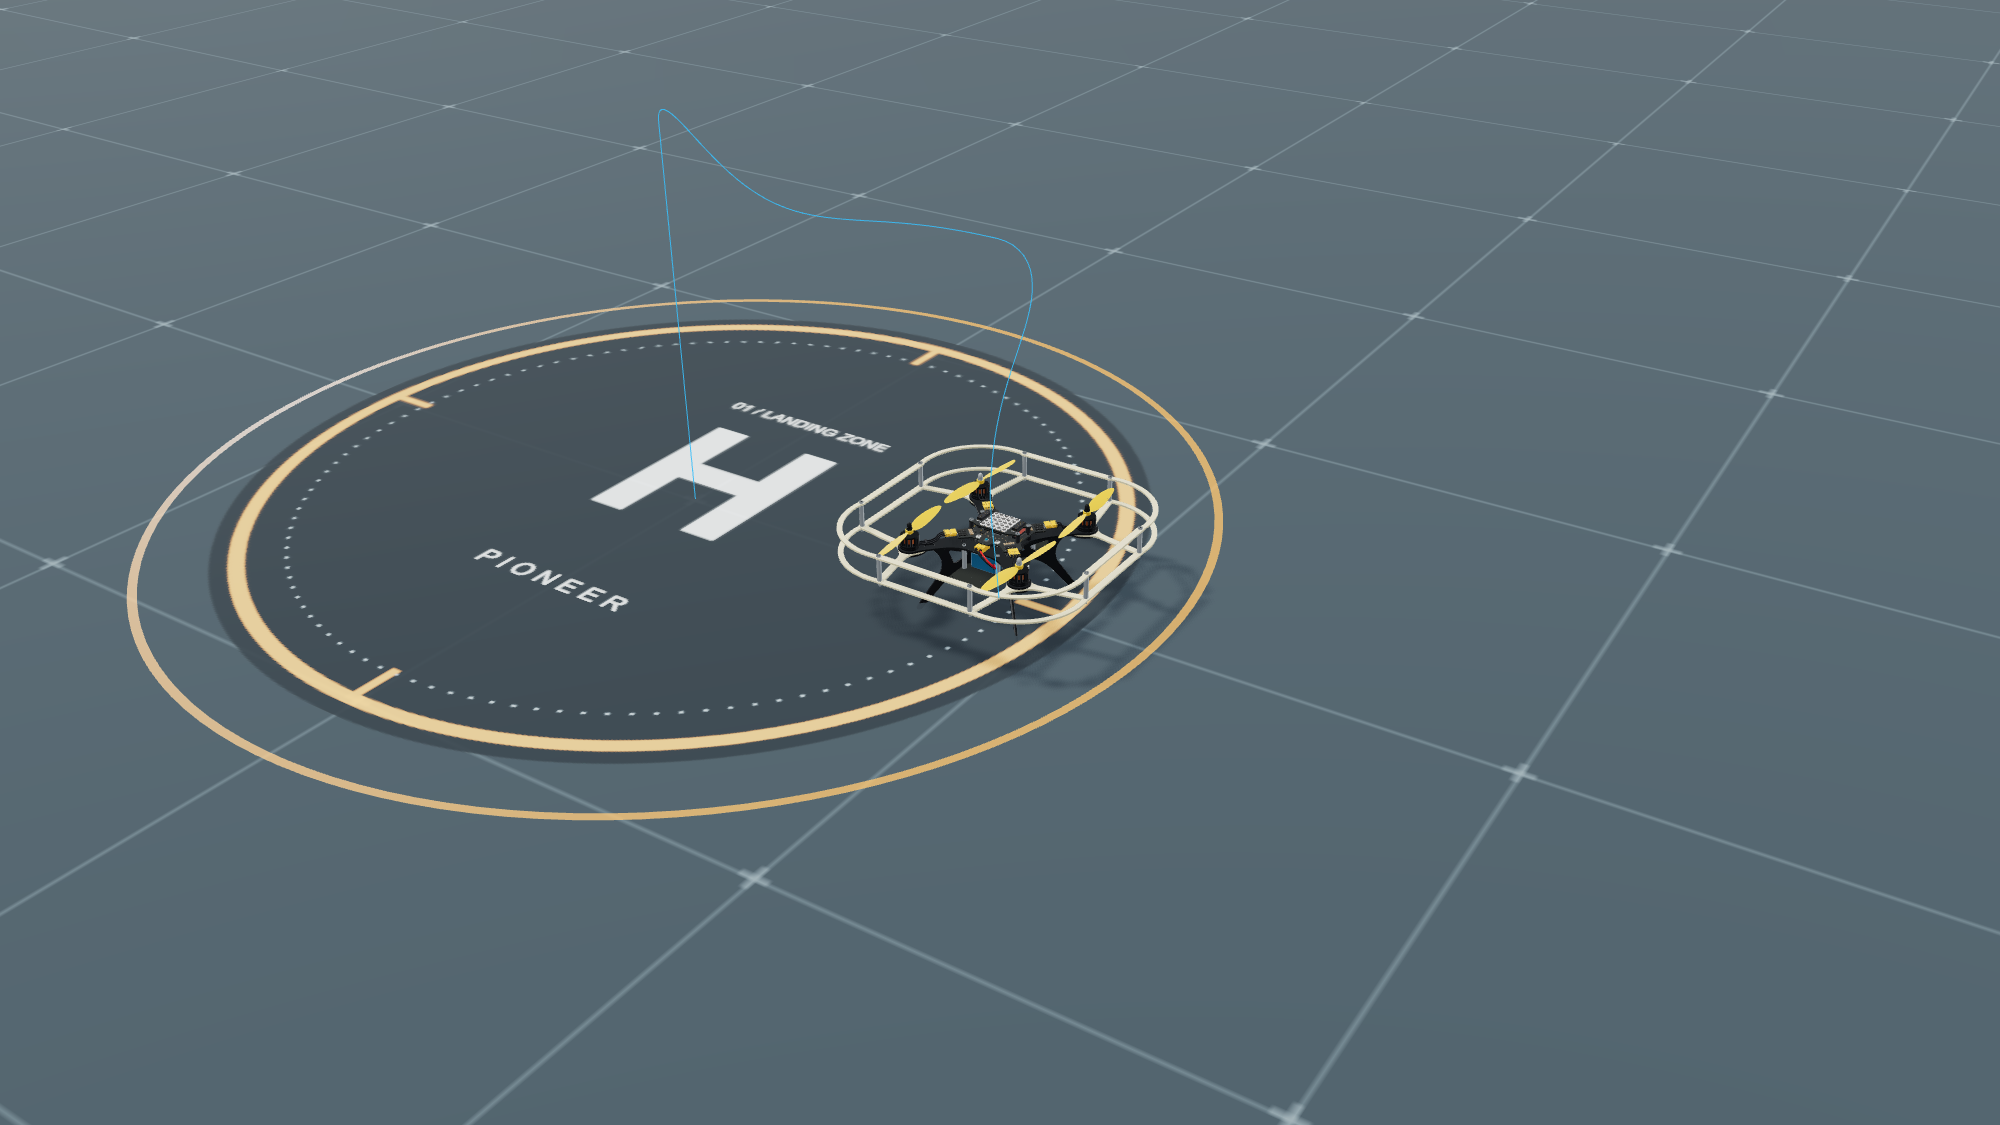
\includegraphics[width=\linewidth, height=0.36\textheight, keepaspectratio]{images/simulator/cover.png}
        \end{tcolorbox}
        \vspace{0.45cm}

        % 4. Что внутри
        \titlechip{Lua}\hspace{4pt}\titlechip{Python}\hspace{4pt}\titlechip{Blockly}\hspace{4pt}\titlechip{Симулятор в браузере}\hspace{4pt}\titlechip{Настоящий дрон}\par
        \vspace{0.45cm}
        {\small\color{GeoskanMuted}\raggedright От первой строки кода до автономной миссии: язык, светодиоды и таймеры, события автопилота, полёт по точкам и фигурам, камера и навигация по маркерам. Каждый пример книги запускается в симуляторе и проверяется автоматически.\par}

        \vfill

        % 5. Автор
        {\large\bfseries\color{GeoskanDarkBlue} #3\par}
        \vspace{3pt}
        {\small\color{GeoskanMuted} #4\par}
        \vspace{0.45cm}

        % 6. Нижняя линейка
        {\color{GeoskanBlue}\rule{\linewidth}{0.6pt}}\par
        \vspace{5pt}
        {\small\color{GeoskanDarkBlue} #5\hfill\texttt{simulator.sakoryagin.ru}\par}
        \vspace{2pt}
        {\footnotesize\color{GeoskanMuted} Версия \theversion\ · сборка \buildtimestamp\par}
    \end{titlepage}
}


\begin{document}

\makePioneerTitle
    {Программирование дронов и создание автономных беспилотных миссий}
    {Курс «Программные средства БПЛА»}
    {Корягин Сергей Андреевич}
    {асп. СПбГЭТУ «ЛЭТИ», педагог ЦО «Кудрово»}
    {г. Кудрово, \the\year}

% Оборот титульного листа: аннотация, адресат, как устроены примеры.
\pagestyle{empty}
\sffamily
\setlength{\parindent}{0pt}
\vspace*{\fill}

{\large\bfseries\color{GeoskanDarkBlue} Корягин С.\,А.}\par
\vspace{4pt}
{\color{GeoskanDarkBlue} Программирование дронов и создание автономных беспилотных миссий: учебное пособие по курсу «Программные средства БПЛА». --- Кудрово, \the\year. --- \pageref{LastPage}~с.}\par
\vspace{1cm}

{\bfseries\color{GeoskanDarkBlue} Аннотация}\par
\vspace{4pt}
Пособие вводит в программирование образовательного квадрокоптера «Геоскан Пионер» на языках Lua и Python. Первая часть --- язык Lua, светодиодная индикация, таймеры и событийная модель автопилота, автономные миссии по точкам и параметрическим траекториям. Вторая часть --- Python и библиотека \texttt{pioneer\_sdk}: подключение, полёт, камера, визуальные маркеры ArUco, трекинг и групповой полёт. Третья часть --- профессиональная навигация: калибровка камеры, карты маркеров, фильтрация измерений. Все программы запускаются в веб-симуляторе \texttt{simulator.sakoryagin.ru} с тем же API, что у настоящего дрона.\par
\vspace{0.8cm}

{\bfseries\color{GeoskanDarkBlue} Для кого}\par
\vspace{4pt}
Для школьников и студентов, начинающих программировать роботов, и педагогов дополнительного образования. Предварительной подготовки по программированию не требуется; математика --- в объёме школьной тригонометрии.\par
\vspace{0.8cm}

{\bfseries\color{GeoskanDarkBlue} Примеры и проверка}\par
\vspace{4pt}
Исходный код всех примеров --- в папке \texttt{examples/} рядом с книгой; каждый файл подписан в тексте. Примеры автоматически прогоняются в симуляторе: взлетают, проходят точки и садятся. Текст примеров можно копировать прямо из PDF.\par
\vspace{0.8cm}

{\footnotesize\color{GeoskanMuted} Версия \theversion\ · сборка \buildtimestamp\par}
\vspace*{\fill}
\clearpage
\pagestyle{scrheadings}

\rmfamily

\tableofcontents
\clearpage

% ------------------------------------------------------------ Введение и старт
\section{Введение: как устроен курс}

\subsection*{О чём эта книга}

Эта книга учит программировать квадрокоптер «Геоскан Пионер»: от первой строчки на языке Lua до автономной миссии, в которой дрон сам взлетает, облетает заданные точки, реагирует на нештатные ситуации и садится. Вторая половина книги делает то же самое на языке Python, а затем выходит за пределы симулятора --- к камере, визуальным маркерам и групповым полётам на настоящем дроне.

Главный принцип курса --- \textbf{каждый пример запускается}. Все программы из книги лежат в папке \texttt{examples/} рядом с текстом и автоматически проверяются в симуляторе: взлетают, пролетают свои точки и садятся. Если пример в книге не совпадает с тем, что вы видите на экране, --- это ошибка книги, а не ваша.

\subsection*{Где писать код}

Для занятий нужен только браузер: веб-симулятор \url{https://simulator.sakoryagin.ru} показывает полёт в 3D, умеет Lua, Python и Blockly и использует тот же API, что настоящий Пионер. Настоящий дрон понадобится ближе к концу курса --- для камеры и компьютерного зрения. Как запускать программы в симуляторе и на дроне, объясняет глава \ref{sec:start}.

\subsection*{Как читать главы}

Каждая глава построена одинаково:
\begin{enumerate}
    \item \textbf{Цели} --- что вы будете уметь после главы.
    \item \textbf{Теория с примерами} --- короткие программы, которые нужно запустить и сверить результат с комментариями в коде.
    \item \textbf{Проверьте себя} --- вопросы с ответами.
    \item \textbf{Практика} --- задания без готового решения; решения к ним лежат в \texttt{examples/lua-tasks/}.
    \item \textbf{Итоги} --- что запомнить.
\end{enumerate}

В тексте встречаются рамки:
\begin{itemize}
    \item \textcolor{GeoskanBlue}{\faInfoCircle}~\textbf{Информация} --- пояснение или ссылка на другой раздел;
    \item \textcolor{red!70!black}{\faExclamationTriangle}~\textbf{Внимание} --- типичная ошибка или вопрос безопасности;
    \item \textcolor{GeoskanOrange}{\faLightbulb}~\textbf{Подсказка} --- приём, который экономит время;
    \item \textcolor{GeoskanDarkBlue}{\faGavel}~\textbf{Правило} --- соглашение, которого курс придерживается всегда.
\end{itemize}

\subsection*{Дорожная карта}

\begin{enumerate}
    \item \textbf{Подготовка.} Интерфейс симулятора, первая программа, настоящий Пионер и техника безопасности.
    \item \textbf{Часть I. Lua.} Язык (переменные, условия, циклы, функции) $\to$ светодиоды и таймеры $\to$ события автопилота и автономные миссии.
    \item \textbf{Часть II. Python.} Основы языка $\to$ библиотека \texttt{pioneer\_sdk}: подключение, светодиоды, взлёт, полёт по точкам $\to$ камера, маркеры ArUco, трекинг, рой.
    \item \textbf{Часть III. Профессиональная навигация.} Теория визуальных маркеров, калибровка камеры, карты, фильтрация и точная посадка.
    \item \textbf{Приложения.} Справочник Lua API, шпаргалка Lua~$\leftrightarrow$~Python, настройка пульта, протокол безопасности.
\end{enumerate}

Lua и Python в курсе идут в одном порядке: сначала язык, потом светодиоды, потом полёт. Поэтому главу про Python можно читать и отдельно, но полезнее --- после Lua: событийная модель автопилота, разобранная на Lua, объясняет, почему Python-программа «ждёт точку» именно так.

\subsection*{Планируемые результаты}

После курса вы сможете:
\begin{itemize}
    \item писать читаемый код на Lua и Python и объяснять, что делает каждая строка;
    \item управлять бортовой периферией --- светодиодами и таймерами --- без блокировки программы;
    \item строить программу полёта как конечный автомат: команда $\to$ событие $\to$ следующая команда;
    \item предусматривать аварийные ситуации: удар, разряд батареи, потеря связи;
    \item переносить программу из симулятора на настоящий дрон без переписывания.
\end{itemize}

\clearpage

\section{Подготовка: где писать и запускать код}
\label{sec:start}

\begin{infobox}[Цели главы]
\begin{itemize}
    \item Понять, чем отличаются запуск в симуляторе и на настоящем дроне, и почему код для них один.
    \item Найти в симуляторе редактор, выбор языка, кнопки запуска и терминал.
    \item Запустить первую программу и увидеть её вывод.
    \item Запомнить правила безопасности при работе с настоящим Пионером.
\end{itemize}
\end{infobox}

\subsection{Два способа запустить программу}

У программы для Пионера есть два «исполнителя»:

\begin{center}
\small
\begin{tabularx}{\linewidth}{@{}>{\bfseries}l X X@{}}
\toprule
 & Симулятор в браузере & Настоящий Пионер \\
\midrule
Что нужно & Любой компьютер с браузером: \url{https://simulator.sakoryagin.ru} & Дрон, аккумулятор, кабель USB или Wi-Fi, площадка \\
Lua & Редактор на сайте, язык \ui{Lua} & Pioneer Station: загрузка скрипта на борт \\
Python & Редактор на сайте, язык \ui{Python} & \texttt{pip install pioneer-sdk}, программа на вашем компьютере \\
Что видно & Полёт в 3D, терминал, телеметрия & Сам дрон и консоль Pioneer Station \\
Цена ошибки & Нажать \ui{Сбросить} & Сломанный пропеллер или хуже \\
\bottomrule
\end{tabularx}
\end{center}

Код в обоих случаях один и тот же: симулятор воспроизводит официальный API автопилота (\texttt{ap}, \texttt{Ev}, \texttt{Timer}, \texttt{Ledbar}, \texttt{Sensors}) и библиотеку \texttt{pioneer\_sdk}. Поэтому в курсе мы сначала отлаживаем программу в симуляторе, а на дрон переносим уже проверенную.

\begin{rulebox}[Сначала симулятор]
Любая новая программа запускается сначала в симуляторе. На настоящем дроне запускается только программа, которая в симуляторе взлетела, выполнила задание и села.
\end{rulebox}

\subsection{Симулятор: что где находится}
\label{sec:simulator-tour}

Откройте \url{https://simulator.sakoryagin.ru}. При первом запуске появится короткая экскурсия --- её можно пройти или пропустить. После неё экран выглядит так:

\begin{shotcallouts}{01-scene.png}
    \callout{0.035}{0.955}{1}
    \callout{0.94}{0.90}{2}
    \callout{0.95}{0.73}{3}
    \callout{0.50}{0.19}{4}
    \callout{0.15}{0.07}{5}
    \callout{0.40}{0.07}{6}
    \callout{0.93}{0.064}{7}
\end{shotcallouts}

\begin{enumerate}[label=\bubble{\arabic*}]
    \item Кнопка панелей. За ней прячется «рельс» с панелями: \ui{Код}, \ui{Полёт} (телеметрия), \ui{Рой}, \ui{Сцена}, \ui{Учебник}, \ui{Пульт}, \ui{Настройки}.
    \item Компас осей. Ось \textbf{X} красная, \textbf{Y} зелёная, \textbf{Z} синяя и смотрит вверх. Щелчок по оси поворачивает камеру вдоль неё.
    \item Окна камер дрона: передняя и нижняя камеры, их же «видит» программа.
    \item \ui{Открыть редактор кода} --- сюда пишется программа. Позже эта кнопка исчезнет, редактор открывается панелью \ui{Код}.
    \item Камера: \ui{Земля} (вид сверху), \ui{Дрон} (камера следует за дроном), \ui{FPV} (от лица дрона), \ui{Свободно} (орбита вокруг точки или свободный полёт камеры).
    \item \ui{Объекты} и \ui{Окружение}: расстановка домов, маркеров, площадок; время суток и погода.
    \item \ui{Запустить}, \ui{Стоп} и \ui{Сбросить}. Сброс возвращает дрон на стартовую площадку и очищает след полёта.
\end{enumerate}

Камеру вращают левой кнопкой мыши, сдвигают правой, приближают колёсиком.

\subsection{Редактор кода}

Нажмите \ui{Открыть редактор кода}. Редактор занимает экран целиком, сцена при этом продолжает жить: программа работает и после закрытия редактора.

\begin{shotcallouts}{02-editor-lua.png}
    \callout{0.035}{0.83}{1}
    \callout{0.098}{0.922}{2}
    \callout{0.245}{0.922}{3}
    \callout{0.46}{0.922}{4}
    \callout{0.83}{0.922}{5}
    \callout{0.876}{0.922}{6}
    \callout{0.903}{0.922}{7}
    \callout{0.931}{0.922}{8}
    \callout{0.968}{0.922}{9}
\end{shotcallouts}

\begin{enumerate}[label=\bubble{\arabic*}]
    \item Рельс панелей: \ui{Код} (этот редактор), \ui{Полёт}, \ui{Рой}, \ui{Сцена}, \ui{Учебник}; внизу --- тема, \ui{Пульт}, \ui{Настройки}.
    \item Язык программы: \ui{Lua}, \ui{Python} или \ui{Blockly}. Переключение не стирает код: у каждого языка своя вкладка.
    \item Готовые примеры --- в том числе все программы из этой книги (папки \texttt{04\_language}, \texttt{05\_leds}, \texttt{06\_missions}).
    \item \ui{Открыть файл} с компьютера и \ui{Скачать код} в файл.
    \item Состояние дрона: \ui{На земле}, \ui{Взлёт}, \ui{В полёте}, \ui{Посадка}.
    \item Справочник API: описание и пример для каждой функции.
    \item Терминал: сюда попадает вывод \texttt{print} и сообщения автопилота.
    \item Уведомления: перед запуском симулятор проверяет программу и объясняет найденные ошибки здесь.
    \item Закрыть редактор и вернуться к сцене. Кнопки \ui{Запустить}, \ui{Стоп}, \ui{Сбросить} --- внизу справа, как и на сцене.
\end{enumerate}

\begin{hintbox}[Пять шагов до запуска]
Открыть редактор $\to$ выбрать язык $\to$ вставить или набрать программу $\to$ \ui{Запустить} $\to$ закрыть редактор и смотреть на сцену. Если дрон ведёт себя не так, как ожидалось, --- \ui{Стоп}, \ui{Сбросить}, и в терминале читать, что произошло.
\end{hintbox}

\subsection{Первая программа}

Традиционно первая программа печатает приветствие. На дроне нет экрана, но есть консоль: в симуляторе это терминал редактора, в Pioneer Station --- окно «Консоль».

\begin{codefile}{lua/02_sensors/getting_started_hello.lua}
\end{codefile}

Выберите язык \ui{Lua}, вставьте программу и нажмите \ui{Запустить}. Затем откройте терминал (значок \texttt{>\_} в заголовке редактора):

\begin{center}
\simshot[0.9\linewidth]{03-terminal.png}
\captionof{figure}{Терминал показывает всё, что программа напечатала через \texttt{print}, и сообщения автопилота.}
\end{center}

Что здесь произошло:
\begin{itemize}
    \item строки, начинающиеся с \texttt{--}, --- комментарии, Lua их не выполняет;
    \item \texttt{print(\dots)} печатает текст в консоль. Текст --- это \textbf{строка}, она записывается в кавычках;
    \item программа закончилась сразу после печати. Дрон не взлетел, потому что мы не дали ему ни одной команды.
\end{itemize}

\begin{taskbox}[Проверка связи]
Измените текст в кавычках на своё имя и запустите программу ещё раз. Затем добавьте вторую строку \texttt{print(2 + 2)} и убедитесь, что Lua умеет считать.
\end{taskbox}

\begin{infobox}[Где лежат примеры]
Каждая программа в книге подписана именем файла, например \texttt{lua/02\_sensors/getting\_started\_hello.lua}. Это путь внутри папки \texttt{examples/} курса. Те же файлы доступны в редакторе симулятора через список примеров, а текст программы можно скопировать прямо из PDF --- отступы и дефисы при копировании сохраняются.
\end{infobox}

\subsection{Настоящий Пионер}

Всё, что отлажено в симуляторе, переносится на дрон. Но дрон --- электромеханическое устройство с вращающимися пропеллерами, поэтому порядок работы с ним строже.

\subsubsection{Техника безопасности}

\begin{warnbox}[Критически важно]
Пренебрежение этими правилами приводит к травмам и поломке оборудования. Они не обсуждаются.
\end{warnbox}

\begin{itemize}
    \item \textbf{Механика --- только без питания.} Любые монтажные работы, замена деталей, подключение модулей --- на обесточенном аппарате.
    \item \textbf{Отладка --- без пропеллеров.} При загрузке и проверке скриптов, тестировании моторов и настройке пульта пропеллеры должны быть сняты. Случайный запуск моторов с пропеллерами --- неконтролируемый взлёт.
    \item \textbf{Аккумуляторы.} Только исправные LiPo-батареи, зарядка под присмотром. Вздувшийся или повреждённый аккумулятор не используется.
    \item \textbf{Порядок включения.} Сначала пульт, потом питание дрона. Выключение --- в обратном порядке.
    \item \textbf{Рабочее место.} На столе нет лишних предметов и проводов; с пропеллерами дрон создаёт сильный поток воздуха.
\end{itemize}

\subsubsection{Pioneer Station}

Основная среда для Lua-программ на настоящем дроне --- \textbf{Pioneer Station}: редактор с подсветкой синтаксиса, загрузчик скриптов на борт, консоль для \texttt{print} и телеметрии, менеджер прошивок. Дистрибутив бесплатно доступен на сайте поддержки Геоскан.

Порядок подключения:
\begin{enumerate}
    \item Убедитесь, что пропеллеры сняты (если вы не планируете немедленный вылет на полигоне).
    \item Подключите аккумулятор. Прозвучит мелодия инициализации, светодиоды начнут мигать.
    \item Соедините дрон с компьютером кабелем micro-USB.
    \item Запустите Pioneer Station и выберите COM-порт (обычно определяется сам).
    \item Вставьте программу в редактор и нажмите «Загрузить». Скрипт передаётся в память автопилота и запускается; результат --- в окне «Консоль».
\end{enumerate}

\subsubsection{Python на настоящем дроне}

Python-программа работает не на борту, а на вашем компьютере, и общается с дроном по Wi-Fi через библиотеку \texttt{pioneer\_sdk}. Установка и подключение разобраны в главе~\ref{sec:python-sdk}. Ту же программу можно направить и на симулятор --- тогда по Wi-Fi полетит виртуальный дрон на сайте (раздел~\ref{sec:python-external}).

\subsubsection{Изучение чистого Lua}

Синтаксис Lua можно тренировать и без дрона: симулятор для этого подходит (терминал показывает \texttt{print}), а на компьютере удобны ZeroBrane Studio, Visual Studio Code с расширением Lua или онлайн-интерпретаторы. Код оттуда для дрона всё равно переносится в симулятор или Pioneer Station.

\subsection*{Итоги}
\begin{itemize}
    \item Программа для Пионера одна, исполнителей два: симулятор в браузере и настоящий дрон.
    \item В симуляторе: редактор $\to$ язык $\to$ \ui{Запустить}; вывод --- в терминале, ошибки --- в уведомлениях.
    \item На дроне: безопасность, Pioneer Station для Lua, \texttt{pioneer\_sdk} для Python.
\end{itemize}

\clearpage

% ============================================================
\part{Программирование на Lua}
% ============================================================

\section{Язык Lua}
\label{sec:lua}

\begin{infobox}[Цели главы]
\begin{itemize}
    \item Различать типы данных Lua и объявлять переменные --- локальные и глобальные.
    \item Записывать арифметику, сравнения и логические условия.
    \item Управлять ходом программы: ветвления \texttt{if}, циклы \texttt{for}, \texttt{while}, \texttt{repeat}.
    \item Писать свои функции и понимать, как автопилот вызывает нашу функцию \texttt{callback}.
    \item Узнавать типичные ошибки новичка по сообщению в терминале.
\end{itemize}
\end{infobox}

\subsection{Зачем Lua}

Lua --- лёгкий встраиваемый язык, созданный в начале 1990-х для расширения программ скриптами. Он компактен, не требует много памяти и быстро работает, поэтому живёт внутри игр, роботов и встраиваемых систем. Автопилот Пионера исполняет Lua прямо на борту: программа загружается в память контроллера и работает без компьютера.

В этом курсе Lua нужен, чтобы:
\begin{itemize}
    \item управлять светодиодами через модуль \texttt{Ledbar} (глава~\ref{sec:leds});
    \item выполнять действия по расписанию через \texttt{Timer}, не останавливая программу;
    \item отвечать на события автопилота --- взлёт завершён, точка достигнута, батарея садится --- в функции \texttt{callback(event)} (глава~\ref{sec:missions}).
\end{itemize}
Сейчас запоминать эти имена не нужно: в этой главе мы работаем только с языком.

\begin{rulebox}[Как работать с главой]
Каждый пример запускайте в симуляторе (язык \ui{Lua}, кнопка \ui{Запустить}) и сверяйте вывод в терминале с комментариями в коде: справа от \texttt{print} написано, что должно появиться.
\end{rulebox}

\subsection{Толковый словарь}
\begin{description}
  \item[\hypertarget{term:number}{Число}] вещественное или целое значение: \verb|3.14|, \verb|10|; математика --- в библиотеке \verb|math|.
  \item[\hypertarget{term:string}{Строка}] текст в кавычках: \verb|"Lua"|; склейка --- оператор \verb|..|, длина --- \verb|#s|.
  \item[\hypertarget{term:boolean}{Булево}] \verb|true| или \verb|false|; результат сравнения и материал для условий.
  \item[\hypertarget{term:nil}{nil}] «ничего»: переменная без значения, отсутствующее поле таблицы.
  \item[\hypertarget{term:table}{Таблица}] единственная составная структура Lua: массив \verb|t[1]| и словарь \verb|t.x| одновременно.
  \item[\hypertarget{term:function}{Функция}] именованный блок кода с параметрами и результатом.
  \item[\hypertarget{term:scope}{Область видимости}] \verb|local| делает переменную видимой только внутри текущего блока; без \verb|local| переменная глобальная --- видна во всём скрипте.
  \item[\hypertarget{term:truthiness}{Истинность}] ложными считаются только \verb|false| и \verb|nil|; ноль и пустая строка --- истина.
  \item[\hypertarget{term:ipairs}{ipairs / pairs}] обход таблицы: \verb|ipairs| --- по номерам 1..N, \verb|pairs| --- по всем ключам в произвольном порядке.
  \item[\hypertarget{term:unpack}{table.unpack}] раскладывает таблицу в список значений: \verb|table.unpack({1,0,0})| даёт \verb|1, 0, 0|. Часто пишут \verb|local unpack = table.unpack|.
\end{description}

\subsection{Переменные и типы}

Переменная --- это имя, за которым закреплено значение. Тип значения определяется автоматически: \hyperlink{term:number}{число}, \hyperlink{term:string}{строка}, \hyperlink{term:boolean}{булево}, \hyperlink{term:table}{таблица}, \hyperlink{term:function}{функция} или \hyperlink{term:nil}{nil}. Узнать тип можно функцией \verb|type()|.

\begin{codefile}{lua/04_language/variables_intro.lua}
\end{codefile}

\paragraph{Что происходит.}
\begin{itemize}
    \item \verb|local x = 10| --- \hyperlink{term:scope}{локальная} переменная: живёт в том блоке, где объявлена.
    \item \verb|name = "Pioneer"| без \verb|local| --- глобальная: её видно из любой функции скрипта. Так в курсе объявляют таймеры (глава~\ref{sec:leds}), которые должны жить до конца программы.
    \item \verb|x, y = 1, 2| присваивает две переменные сразу, а \verb|x, y = y, x| меняет их местами без третьей переменной.
    \item \verb|print(type(x), ...)| печатает имена типов через табуляцию.
\end{itemize}

\subsubsection*{Таблицы}

Таблица --- и массив, и словарь. Позиционные элементы нумеруются \textbf{с единицы}, именованные поля доступны через точку.

\begin{codefile}{lua/04_language/lua_variables_tables.lua}
\end{codefile}

\begin{itemize}
    \item \verb|#a| --- длина массива. После \verb|a[4] = 40| она равна 4.
    \item Присваивание \verb|t.speed = nil| удаляет поле из таблицы.
    \item Таблицами в курсе задаются цвета \verb|{1, 0, 0}| и точки маршрута \verb|{x, y, z}|.
\end{itemize}

\begin{rulebox}[local по умолчанию]
Объявляйте переменные через \verb|local|. Глобальными оставляйте только то, что должно жить всю программу: таймеры и обязательную функцию \verb|callback| (о ней --- в разделе «Функции» этой главы). Переменная, объявленная через \verb|local| в самом начале файла, тоже живёт всю программу и видна всем функциям ниже, --- так в миссиях хранят текущее состояние (глава~\ref{sec:missions}).
\end{rulebox}

\subsubsection*{Задачи для самостоятельного решения}
\begin{enumerate}
  \item Объявите локальную переменную \verb|x| со значением \verb|42| и напечатайте её.
  \item Создайте таблицу \verb|t| с полем \verb|speed = 3.5| и элементами \verb|1, 2, 3|; напечатайте \verb|t.speed| и \verb|#t|.
  \item Добавьте в \verb|t| поле \verb|mode = "auto"|, затем удалите поле \verb|speed|.
  \item Создайте таблицу \verb|color = {r = 1, g = 0, b = 0}| и напечатайте её поля одной командой \verb|print|.
  \item Объявите \verb|local a, b = 1, 2|, поменяйте значения местами одной строкой и напечатайте результат.
  \item Напечатайте \verb|type(nil)|, \verb|type("5")| и \verb|type(5)|. Чем отличаются два последних?
\end{enumerate}

\subsection{Арифметика и сравнения}

Операции: \verb|+ - * / %| (остаток от деления) и \verb|^| (степень). Сравнения: \verb|< <= > >= ==| и \verb|~=| («не равно»). Приоритет как в математике: сначала \verb|^|, затем \verb|* / %|, потом \verb|+ -|; скобки меняют порядок.

\begin{codefile}{lua/04_language/lua_arithmetic_ops.lua}
\end{codefile}

\paragraph{Что происходит.}
\begin{itemize}
    \item \verb|2 ^ 3| даёт \verb|8.0|, а не \verb|8|: степень и деление \verb|/| всегда возвращают вещественное число. Целые и вещественные числа в Lua~5.3 --- два подвида одного типа, в арифметике они смешиваются свободно.
    \item Оператора \verb|**| в Lua нет --- это Python. Степень только через \verb|^|.
    \item \verb|math.floor(17 / 4)| --- целочисленное деление с округлением вниз. В симуляторе работает и \verb|//|, но \verb|math.floor| переносимее.
    \item \verb|math.sqrt|, \verb|math.abs|, \verb|math.max|, \verb|math.min|, \verb|math.pi| --- то, что понадобится в миссиях. Тригонометрия Lua и автопилот измеряют углы в \textbf{радианах}: полный оборот --- $2\pi \approx 6.28$~рад, $180^\circ = \pi$. Перевод градусов в радианы: \verb|math.rad(deg)|, обратно --- \verb|math.deg(rad)|.
\end{itemize}

\begin{hintbox}[Ограничить значение диапазоном]
\verb|v = math.max(0, math.min(1, v))| «зажимает» \verb|v| между 0 и 1. Этот приём пригодится для яркости светодиодов.
\end{hintbox}

\subsubsection*{Задачи для самостоятельного решения}
\begin{enumerate}
  \item Напечатайте \verb|3 + 4 * 2 - 5| и \verb|(3 + 4) * (2 - 5)|.
  \item Напечатайте остаток \verb|17 % 4| и проверьте условием, чётно ли число \verb|n = 10|.
  \item Вычислите длину вектора \verb|(x, y) = (3, 4)| через \verb|math.sqrt(x*x + y*y)|.
  \item Переведите \verb|90| градусов в радианы двумя способами: \verb|deg * math.pi / 180| и \verb|math.rad(deg)|. Сравните результаты.
  \item Реализуйте линейную интерполяцию \verb|lerp = a + t * (b - a)| для \verb|a = 0|, \verb|b = 10|, \verb|t = 0.25|.
  \item Напечатайте среднее трёх чисел \verb|(a + b + c) / 3|.
\end{enumerate}

\subsection{Логические операции}

Логика: \verb|and| (И), \verb|or| (ИЛИ), \verb|not| (НЕ). Ложными считаются только \verb|false| и \verb|nil| (\hyperlink{term:truthiness}{истинность}): число \verb|0| и пустая строка --- истина. Операторы \verb|and| и \verb|or| вычисляют правую часть только при необходимости («короткое замыкание»).

\begin{codefile}{lua/04_language/lua_logic_ops.lua}
\end{codefile}

\paragraph{Что происходит.}
\begin{itemize}
    \item \verb|gt and 1 or 0| --- идиома «если \verb|gt|, то 1, иначе 0». В Lua нет тернарного оператора, его заменяет эта пара.
    \item \verb|(a >= 0) and (a <= 100)| --- проверка диапазона. Запись \verb|0 <= a <= 100| в Lua не работает.
    \item \verb|name ~= nil and name ~= ""| --- сначала убеждаемся, что значение есть, и только потом сравниваем со строкой. Так защищаются от \verb|nil|.
    \item Строки сравниваются лексикографически: \verb|"a" < "b"| истинно.
\end{itemize}

\subsubsection*{Задачи для самостоятельного решения}
\begin{enumerate}
  \item Для \verb|voltage = 3.4| и \verb|temp = 85| напечатайте «сигнал опасности»: \verb|voltage < 3.5 or temp > 80|.
  \item Напишите предикат «индекс чётный» для \verb|i = 7|: \verb|i % 2 == 0|.
  \item Выберите максимум из \verb|a| и \verb|b| одной строкой через \verb|and/or|.
  \item Инвертируйте булеву переменную \verb|on| и напечатайте её до и после.
  \item Проверьте закон де Моргана: напечатайте \verb|not (p and q)| и \verb|(not p) or (not q)| для всех четырёх сочетаний \verb|p|, \verb|q|.
  \item Напишите условие «\verb|t| не \verb|nil| и у \verb|t| есть поле \verb|value|».
\end{enumerate}

\subsection{Условия}

Ветвление записывается словами \texttt{if} \dots\ \texttt{then} \dots\ \texttt{elseif} \dots\ \texttt{then} \dots\ \texttt{else} \dots\ \texttt{end}. Ветка \verb|elseif| может повторяться, \verb|else| --- не обязательна, \verb|end| --- обязателен всегда.

\begin{codefile}{lua/04_language/lua_conditions_if.lua}
\end{codefile}

\paragraph{Что происходит.} Функция \verb|classify| проверяет условия по порядку и возвращает первое подходящее слово. Для \verb|0| первая проверка \verb|x > 0| ложна, вторая \verb|x == 0| истинна --- получаем \verb|"zero"|.

\subsubsection*{Охранное условие}

Обращение к полю несуществующей таблицы --- ошибка «attempt to index a nil value». Защищаются от неё проверкой перед обращением:

\begin{codefile}{lua/04_language/lua_conditions_check.lua}
\end{codefile}

Условие \verb|t and t.value| читается так: «\verb|t| существует, и у неё есть поле \verb|value|». Если \verb|t| равно \verb|nil|, до \verb|t.value| дело не доходит --- спасает короткое замыкание \verb|and|.

\begin{hintbox}[Таблица вместо каскада if]
Когда вариантов много и каждому соответствует действие, удобнее таблица: \verb|colors[state]| или даже таблица функций \verb|actions[state]()|. Так в главе~\ref{sec:leds} устроен светофор --- самый маленький конечный автомат.
\end{hintbox}

\subsubsection*{Задачи для самостоятельного решения}
\begin{enumerate}
  \item Напишите функцию, которая для напряжения \verb|v| возвращает \verb|"low"| при \verb|v < 3.7| и \verb|"ok"| иначе. Проверьте на 3.5 и 4.1.
  \item Присвойте \verb|parity| значение \verb|"even"| при чётном \verb|n| и \verb|"odd"| при нечётном.
  \item Тройное ветвление по температуре: \verb|temp < 0| $\to$ \verb|"cold"|, \verb|0 <= temp < 20| $\to$ \verb|"cool"|, иначе \verb|"warm"|.
  \item Напишите ветвление, выбирающее цвет: \verb|{1,0,0}| для \verb|state == "RED"|, \verb|{1,1,0}| для \verb|"YELLOW"|, иначе \verb|{0,1,0}|.
  \item Защитите деление от нуля: если \verb|b ~= 0|, напечатайте \verb|a / b|, иначе --- сообщение об ошибке.
  \item Если \verb|count == 0|, присвойте \verb|count = 1|, иначе увеличьте на 1.
\end{enumerate}

\subsection{Циклы}

Три вида повторения: числовой \verb|for| (счётчик от начала до конца включительно, с шагом), \verb|while| (пока условие истинно) и \verb|repeat ... until| (тело выполняется хотя бы один раз). Для таблиц есть \verb|for ... in ipairs(a)| и \verb|for ... in pairs(t)|.

\begin{codefile}{lua/04_language/loops_sum.lua}
\end{codefile}

Границы \verb|for i = 1, 10| включительны: \verb|i| принимает значения от 1 до 10. Светодиоды линейки (29 штук, глава~\ref{sec:leds}) нумеруются с нуля, поэтому их обходят циклом \verb|for i = 0, 28 do|.

\begin{codefile}{lua/04_language/loops_while.lua}
\end{codefile}

\begin{codefile}{lua/04_language/loops_iterators.lua}
\end{codefile}

\paragraph{Что происходит.}
\begin{itemize}
    \item \verb|ipairs| перебирает массив по порядку и останавливается на первом «пропуске» (\verb|nil|); \verb|pairs| перебирает все ключи словаря, порядок не гарантирован.
    \item \verb|break| прерывает цикл. Оператора \verb|continue| в Lua нет --- вместо него условие внутри тела.
\end{itemize}

\begin{warnbox}[Вечный цикл останавливает дрон]
Цикл \verb|while true do ... end| без выхода никогда не вернёт управление автопилоту: события перестанут приходить, таймеры --- срабатывать. Повторяющиеся действия на дроне делают таймером \verb|Timer.new| (глава~\ref{sec:leds}), а не бесконечным циклом. Симулятор не даст запустить такую программу и объяснит почему.
\end{warnbox}

\begin{codefile}{lua/04_language/lua_platform_infinite_loop.lua}
\end{codefile}

\subsubsection*{Задачи для самостоятельного решения}
\begin{enumerate}
  \item Посчитайте сумму чисел от 1 до 100.
  \item Найдите максимум в массиве \verb|a = {3, 9, 2, 7}|.
  \item Постройте массив \verb|b| из квадратов элементов \verb|a|.
  \item Вычислите факториал \verb|n = 6| циклом \verb|while|.
  \item Заполните таблицу \verb|idx| значениями от 0 до 28 (как номера светодиодов) и напечатайте \verb|#idx|.
  \item Постройте массив из первых 10 чисел Фибоначчи.
  \item Скопируйте словарь \verb|t = {x = 1, y = 2}| в \verb|copy|, увеличив каждое значение на 1.
\end{enumerate}

\subsection{Функции}

Функция --- именованный блок кода, который принимает параметры и возвращает результат. Объявляется словом \verb|function|, заканчивается \verb|end|, результат отдаёт \verb|return|.

\begin{codefile}{lua/04_language/lua_functions.lua}
\end{codefile}

\paragraph{Что происходит.}
\begin{itemize}
    \item \verb|local function average(a, b)| --- локальная функция: видна только в этом файле ниже объявления. Вызов \verb|average(1, 2)| подставляет \verb|a = 1|, \verb|b = 2| и возвращает \verb|1.5|.
    \item Функция может вернуть несколько значений: \verb|return color, word|. Так устроены датчики дрона: \verb|local x, y, z = Sensors.lpsPosition()| возвращает три координаты сразу (все датчики --- в приложении~\ref{sec:lua-api}).
    \item Функцию можно передать как значение. Например, \verb|Timer.callLater(3, blink)| просит вызвать функцию \verb|blink| через 3~секунды (таймеры разобраны в главе~\ref{sec:leds}): сюда передаётся сама функция \verb|blink|, а \verb|Timer.callLater(3, blink())| передал бы результат её вызова. Второе --- ошибка, симулятор её ловит.
\end{itemize}

\subsubsection*{Функция, которую вызываем не мы}

Обычно функцию вызывает наша программа. Но есть функция, которую вызывает \textbf{автопилот}:

\begin{codebox}[Обработчик событий]
\begin{verbatim}
function callback(event)
  -- сюда автопилот передаёт событие:
  -- взлёт завершён, точка достигнута, дрон сел...
end
\end{verbatim}
\end{codebox}

Мы только определяем её --- глобально, без \verb|local|, ровно с таким именем. Когда произойдёт событие, автопилот сам вызовет \verb|callback| и передаст номер события. Что с ним делать, разбирают главы~\ref{sec:leds} и~\ref{sec:missions}; пока запомните: \textbf{в каждой программе, которая командует автопилотом, есть \texttt{callback}}, даже пустой. Программам, которые только зажигают светодиоды, он не нужен.

\subsubsection*{Задачи для самостоятельного решения}
\begin{enumerate}
  \item Напишите функцию \verb|square(x)|, возвращающую квадрат числа; проверьте на 5.
  \item Напишите \verb|isEven(n)|, возвращающую \verb|true| для чётных чисел.
  \item Напишите \verb|clamp(v, lo, hi)|, ограничивающую \verb|v| диапазоном \verb|[lo, hi]|.
  \item Напишите \verb|toRadians(deg)| и проверьте, что \verb|toRadians(180)| равно \verb|math.pi|.
  \item Напишите \verb|polar(r, deg)|, возвращающую две координаты \verb|x, y| точки окружности радиуса \verb|r| под углом \verb|deg| градусов.
  \item Напишите функцию \verb|describeBattery(v)|: ниже 3.5~В --- \verb|"critical"|, ниже 3.8 --- \verb|"low"|, иначе \verb|"ok"|.
\end{enumerate}

\subsection{Типичные ошибки и их сообщения}

Терминал симулятора и консоль Pioneer Station показывают текст ошибки и номер строки. Самые частые:

\begin{center}
\small
\begin{tabularx}{\linewidth}{@{}>{\ttfamily}l X@{}}
\toprule
\normalfont\textbf{Сообщение} & \textbf{Причина и лечение} \\
\midrule
attempt to call a nil value (global 'Print') & Регистр букв: \texttt{Print}, \texttt{PRINT} и \texttt{print} --- три разных имени. Все функции языка пишутся строчными; с заглавной --- только модули \texttt{Ledbar}, \texttt{Timer}, \texttt{Sensors}, \texttt{Ev}. \\
attempt to index a nil value & Обращение к полю переменной, в которой \texttt{nil}: таблица не создана или опечатка в имени. Проверьте объявление и используйте охранное условие. \\
attempt to compare nil with number & Переменная не получила значения до сравнения --- например, опечатка в имени или \texttt{local} внутри другого блока. \\
'end' expected & Не хватает \texttt{end}: у каждого \texttt{if}, \texttt{for}, \texttt{while}, \texttt{function} свой \texttt{end}. Выравнивайте код отступами --- так пропуск виден. \\
unexpected symbol near '**' & Степень в Lua --- \texttt{\^{}}, а не \texttt{**}. \\
\bottomrule
\end{tabularx}
\end{center}

\begin{warnbox}[Индексы: с нуля или с единицы]
Таблицы Lua нумеруются с \textbf{1}: \texttt{points[1]} --- первая точка. Светодиоды --- аппаратный модуль, они нумеруются с \textbf{0}: \texttt{leds:set(0, ...)} --- первый светодиод. Путаница между ними --- самая частая ошибка следующей главы.
\end{warnbox}

\subsection{Проверьте себя}
\begin{enumerate}
  \item Что напечатает \verb|print(10 / 2)|?
    \begin{enumerate}[label=(\alph*)] \item \verb|5| \item \verb|5.0| \item \verb|5,0| \end{enumerate}
    Ответ: (b) --- деление всегда даёт вещественное число.
  \item Какое из значений ложно в условии \verb|if|?
    \begin{enumerate}[label=(\alph*)] \item \verb|0| \item \verb|""| \item \verb|nil| \end{enumerate}
    Ответ: (c) --- ложны только \verb|false| и \verb|nil|.
  \item Чему равно \verb|#{10, 20, 30}|?
    \begin{enumerate}[label=(\alph*)] \item \verb|2| \item \verb|3| \item \verb|30| \end{enumerate}
    Ответ: (b).
  \item Сколько раз выполнится тело \verb|for i = 0, 28 do|?
    \begin{enumerate}[label=(\alph*)] \item 28 \item 29 \item 27 \end{enumerate}
    Ответ: (b) --- обе границы включительно.
  \item Какой из вызовов передаёт функцию, а не результат её вызова?
    \begin{enumerate}[label=(\alph*)] \item \verb|Timer.callLater(2, blink())| \item \verb|Timer.callLater(2, blink)| \end{enumerate}
    Ответ: (b).
  \item Что делает \verb|x, y = y, x|?
    \begin{enumerate}[label=(\alph*)] \item Ошибка \item Меняет значения местами \item Присваивает обеим \verb|y| \end{enumerate}
    Ответ: (b).
\end{enumerate}

\subsection*{Итоги главы}
\begin{itemize}
    \item Переменные объявляются через \verb|local|; глобальные --- только для долгоживущего состояния.
    \item Таблица --- массив (с 1) и словарь одновременно; цвета и точки маршрута --- таблицы.
    \item Ложны только \verb|false| и \verb|nil|; \verb|cond and A or B| заменяет тернарный оператор.
    \item Циклы \verb|for|, \verb|while|, \verb|repeat|; бесконечный цикл на дроне недопустим --- вместо него таймер.
    \item Функции возвращают несколько значений и передаются как аргументы; \verb|callback(event)| вызывает автопилот.
\end{itemize}

\clearpage

\section{Светодиоды и таймеры}
\label{sec:leds}

\begin{infobox}[Цели главы]
\begin{itemize}
    \item Понять, как устроена светодиодная линейка Пионера и почему её адреса --- \texttt{0..28}.
    \item Задавать цвет через модуль \texttt{Ledbar} и модель RGB.
    \item Делать анимации на таймерах \texttt{Timer.new} и \texttt{Timer.callLater}, не останавливая программу.
    \item Реагировать на события автопилота в \texttt{callback(event)}.
    \item Строить индикацию как конечный автомат: состояние $\to$ событие $\to$ переход.
\end{itemize}
\end{infobox}

\subsection{Зачем дрону светодиоды}

Светодиоды --- первый видимый результат программы: дрон стоит на земле, а цвет меняется. Поэтому с них начинают. Но это ещё и рабочий инструмент: по цвету понятно, в каком состоянии программа --- готовится, летит, садится, сообщает об ошибке, --- даже когда терминала нет рядом. В главе~\ref{sec:missions} мы будем подсвечивать этапы миссии именно так.

В этой главе дрон не взлетает. Все примеры безопасно запускать и в симуляторе, и на настоящем Пионере со снятыми пропеллерами.

\subsection{Толковый словарь}
\begin{description}
  \item[\hypertarget{term:ledbar}{Ledbar}] модуль управления RGB-светодиодами: \verb|Ledbar.new(N)| создаёт объект, \verb|leds:set(i, r, g, b)| задаёт цвет.
  \item[\hypertarget{term:rgb}{RGB}] три компоненты цвета --- красная, зелёная, синяя --- числа от \verb|0.0| (выключено) до \verb|1.0| (максимум).
  \item[\hypertarget{term:index}{Индекс светодиода}] номер в линейке, от \verb|0| до \verb|N-1|.
  \item[\hypertarget{term:timer}{Таймер}] «будильник», который вызывает функцию через заданное время (\verb|Timer.callLater|) или периодически (\verb|Timer.new|).
  \item[\hypertarget{term:tick}{Тик}] один вызов функции таймера.
  \item[\hypertarget{term:event}{Событие}] сигнал от автопилота --- взлёт завершён, точка достигнута, батарея разряжена. Передаётся в \verb|callback(event)| как значение \verb|Ev.*|.
  \item[\hypertarget{term:state}{Состояние}] текущий режим логики программы, например \verb|"RED"| или \verb|"FLIGHT"|; хранится в переменной.
  \item[\hypertarget{term:automaton}{Конечный автомат}] программа, которая всегда находится ровно в одном состоянии и переходит в другое только по событию.
  \item[\hypertarget{term:blocking}{Блокирующий вызов}] функция, которая останавливает всю программу, пока не завершится, например \verb|sleep(t)|.
\end{description}

\subsection{Аппаратная часть: 4 + 25 светодиодов}

На плате Пионера четыре RGB-светодиода --- по одному у каждого луча. Модуль светодиодной матрицы добавляет ещё 25. Программа видит их как одну линейку: индексы \verb|0..3| --- светодиоды платы, \verb|4..28| --- модуль. Всего 29, поэтому в курсе линейка всегда создаётся как \verb|Ledbar.new(29)|: на дроне без модуля лишние индексы просто ни на что не влияют, а в симуляторе отображаются все 29.

\begin{center}
\begin{tikzpicture}[scale=1.1]
    \draw[fill=gray!10, thick, rounded corners] (-1.5,-1.5) rectangle (1.5,1.5);
    \node at (0,0.35) {\textbf{Pioneer}};
    \node[font=\footnotesize] at (0,-0.15) {(вид сверху)};
    \draw[->, ultra thick, GeoskanBlue] (0, 1.6) -- (0, 2.6) node[above, font=\footnotesize\bfseries] {Вперёд, ось X};
    \foreach \x/\y in {1.5/1.5, 1.5/-1.5, -1.5/1.5, -1.5/-1.5} { \draw[thick, double] (\x,\y) -- (1.6*\x,1.6*\y); }
    \foreach \x/\y in {2.4/2.4, 2.4/-2.4, -2.4/2.4, -2.4/-2.4} { \draw[fill=black!15] (\x,\y) circle (0.55); }
    \node[circle, fill=red!70, inner sep=3pt, label=left:{\ttfamily 0}] at (-1.1, 1.1) {};
    \node[circle, fill=green!70!black, inner sep=3pt, label=right:{\ttfamily 1}] at (1.1, 1.1) {};
    \node[circle, fill=blue!70, inner sep=3pt, label=right:{\ttfamily 2}] at (1.1, -1.1) {};
    \node[circle, fill=yellow!80!black, inner sep=3pt, label=left:{\ttfamily 3}] at (-1.1, -1.1) {};
    \node[font=\footnotesize, align=center] at (0,-3.4) {Индексы \texttt{0..3} --- плата; \texttt{4..28} --- модуль матрицы.\\ Какой индекс какому углу соответствует, проверяет задание ниже.};
\end{tikzpicture}
\end{center}

\subsubsection*{Модель RGB}

Цвет --- три числа от \verb|0.0| до \verb|1.0|: красный, зелёный, синий. Смешивая каналы, получаем любой оттенок:

\begin{center}
\small
\begin{tabular}{@{}llll@{}}
\toprule
\verb|{1, 0, 0}| красный & \verb|{0, 1, 0}| зелёный & \verb|{0, 0, 1}| синий & \verb|{1, 1, 0}| жёлтый \\
\verb|{1, 0, 1}| фиолетовый & \verb|{0, 1, 1}| бирюзовый & \verb|{1, 1, 1}| белый & \verb|{0, 0, 0}| выключен \\
\bottomrule
\end{tabular}
\end{center}

Значения меньше единицы --- тусклее: \verb|{0.2, 0, 0}| --- тёмно-красный. В Python светодиодами управляет метод \verb|led_control| библиотеки \texttt{pioneer\_sdk}, и компоненты там --- целые числа \verb|0..255| (глава~\ref{sec:python-sdk}); в Lua --- только \verb|0..1|.

\subsection{Модуль Ledbar}

\begin{codebox}[Две функции, которых достаточно]
\begin{itemize}
  \item \verb|local leds = Ledbar.new(29)| --- создать объект линейки из 29 светодиодов. Вызывается один раз в начале программы.
  \item \verb|leds:set(i, r, g, b)| --- задать цвет светодиода \verb|i| (от \verb|0| до \verb|28|). Обратите внимание на двоеточие: \verb|set| --- метод объекта \verb|leds|.
\end{itemize}
\end{codebox}

\begin{codefile}{lua/05_leds/leds_basic_green.lua}
\end{codefile}

\paragraph{Что происходит.} Функция \verb|changeColor| принимает таблицу \verb|{r, g, b}|, а \verb|unpack| раскладывает её в три аргумента \verb|leds:set|. Цикл \verb|for i = 0, ledNumber - 1| обходит все 29 индексов. Один вызов \verb|changeColor({0, 1, 0})| --- и вся линейка зелёная.

\begin{warnbox}[Индекс вне диапазона не вызывает ошибку]
\verb|leds:set(29, ...)| на линейке из 29 элементов молча игнорируется: светодиод не загорится, а программа продолжит работать. Если какой-то светодиод «не светится», первым делом проверьте индекс.
\end{warnbox}

\subsubsection*{Исследование: какой индекс где}

\begin{codefile}{lua/05_leds/leds_addressing_research.lua}
\end{codefile}

\begin{taskbox}[Карта светодиодов]
Запустите программу: загорится светодиод с индексом \verb|0|. Посмотрите на дрон (в симуляторе --- камерой \ui{Дрон}): какой это угол? Замените \verb|0| на \verb|1|, \verb|2|, \verb|3| и заполните таблицу. Если есть модуль матрицы --- продолжите до \verb|28|.
\end{taskbox}

\begin{center}
\renewcommand{\arraystretch}{1.4}
\begin{tabular}{|c|p{7cm}|}
\hline
\rowcolor{GeoskanBlue!20} \textbf{Индекс} & \textbf{Расположение} \\
\hline
0 & \dotfill \\ \hline
1 & \dotfill \\ \hline
2 & \dotfill \\ \hline
3 & \dotfill \\ \hline
4 \dots 28 & \dotfill \\ \hline
\end{tabular}
\end{center}

Это упражнение учит главному принципу инженера: если документации недостаточно --- проведи эксперимент.

\subsection{Время: почему не sleep}

Чтобы цвет менялся, нужно время. Первое, что приходит в голову, --- остановить программу на секунду функцией \verb|sleep|:

\begin{codefile}{lua/05_leds/leds_sleep.lua}
\end{codefile}

Запустите: красный, через секунду зелёный, ещё через секунду линейка гаснет. Работает. Но пока \verb|sleep| «спит», программа \hyperlink{term:blocking}{не делает ничего другого}: не принимает события автопилота, не обслуживает другие таймеры, не читает датчики. На земле это терпимо, в полёте --- нет: дрон не узнает, что долетел до точки, и не отреагирует на разряд батареи.

\begin{rulebox}[Без sleep]
В программах для дрона \verb|sleep| не используется. Пауза --- это таймер: «через $t$ секунд сделай вот это», а программа тем временем свободна.
\end{rulebox}

\subsection{Таймеры}

\begin{codebox}[API таймеров]
\begin{itemize}
  \item \verb|Timer.callLater(delay, fn)| --- вызвать \verb|fn| один раз через \verb|delay| секунд.
  \item \verb|t = Timer.new(period, fn)| --- создать периодический таймер: \verb|fn| вызывается каждые \verb|period| секунд, пока таймер запущен.
  \item \verb|t:start()| и \verb|t:stop()| --- запустить и остановить периодический таймер.
\end{itemize}
Время всегда в секундах: \verb|0.5| --- полсекунды.
\end{codebox}

\subsubsection*{Отложенное действие}

\begin{codefile}{lua/05_leds/leds_timers_delayed.lua}
\end{codefile}

Программа заканчивается сразу, но через 3 секунды автопилот вызывает переданную функцию, и линейка загорается синим. Обратите внимание: в \verb|callLater| передаётся \emph{функция}, а не результат её вызова.

\subsubsection*{Периодическое действие: мигание}

\begin{codefile}{lua/05_leds/leds_timers_blink.lua}
\end{codefile}

\paragraph{Что происходит.} Переменная \verb|on| хранит \hyperlink{term:state}{состояние} мигалки. Каждые 0.5~с функция \verb|updateBlink| сначала выставляет цвет по текущему состоянию (\verb|on and 1 or 0| --- единица, если \verb|on| истинно), а затем меняет состояние на противоположное (\verb|on = not on|) --- на следующем тике цвет будет другим. Первый тик линейку гасит, второй зажигает красным, и так по кругу. Таймер \verb|blinkTimer| объявлен глобально --- так он живёт до конца программы, и его можно остановить из любой функции.

\begin{hintbox}[Один тик --- один шаг]
Функция таймера должна делать один короткий шаг анимации и возвращаться. Никаких циклов ожидания внутри: следующий шаг таймер вызовет сам.
\end{hintbox}

\subsubsection*{Задачи}
\begin{enumerate}
  \item Измените период мигания на 0.2~с и цвет на синий.
  \item Через 2~с после запуска включите зелёный, через 4~с --- выключите (два \verb|callLater|).
  \item «Бегущий огонёк»: таймер с периодом 0.1~с зажигает только один светодиод, индекс которого увеличивается на 1 и после 28 возвращается к 0.
\end{enumerate}

\subsection{События автопилота}

Таймер --- это событие «прошло время». Автопилот умеет сообщать и о других событиях: моторы запущены, взлёт завершён, точка достигнута, дрон сел, батарея разряжена, удар. Для них есть одна функция:

\begin{codebox}[Обработчик событий]
\begin{verbatim}
function callback(event)
  if event == Ev.COPTER_LANDED then
    -- что сделать после посадки
  end
end
\end{verbatim}
\end{codebox}

Мы её только определяем. Вызывает её автопилот --- каждый раз, когда что-то произошло, --- и передаёт в \verb|event| код события. Коды хранятся в таблице \verb|Ev|; сравнивать нужно именно с \verb|Ev.ИМЯ|, а не с числом.

\begin{center}
\small
\begin{tabularx}{\linewidth}{@{}>{\ttfamily}l X@{}}
\toprule
\normalfont\textbf{Событие} & \textbf{Когда приходит} \\
\midrule
Ev.ENGINES\_STARTED & моторы запущены после предстартовой подготовки \\
Ev.TAKEOFF\_COMPLETE & взлёт завершён, дрон висит на высоте взлёта \\
Ev.POINT\_REACHED & достигнута точка, заданная \texttt{ap.goToLocalPoint} \\
Ev.COPTER\_LANDED & дрон коснулся земли после посадки \\
Ev.LOW\_VOLTAGE1, Ev.LOW\_VOLTAGE2 & батарея разряжена: первый порог --- предупреждение, второй --- пора садиться \\
Ev.SHOCK & удар или столкновение \\
\bottomrule
\end{tabularx}
\end{center}

\subsubsection*{Реакция на посадку}

\begin{codefile}{lua/05_leds/leds_events_landed.lua}
\end{codefile}

Линейка горит белым всё время работы и гаснет, когда автопилот сообщит о посадке. В симуляторе проверить это можно так: добавьте в начало программы взлёт и посадку из главы~\ref{sec:missions} --- или запустите готовый пример \texttt{leds\_mission\_stages.lua} из следующего раздела.

\subsubsection*{Реакция на разряд батареи}

\begin{codefile}{lua/05_leds/leds_events_low_voltage.lua}
\end{codefile}

\paragraph{Что происходит.} В штатном режиме таймер мигает зелёным. Событие \verb|LOW_VOLTAGE2| останавливает таймер и через секунду заливает линейку красным. Пауза нужна, потому что уже запланированный тик таймера может сработать ещё раз сразу после \verb|stop()| --- так устроен автопилот Пионера.

Короткий вариант того же приёма, без таймера мигания. Останавливать здесь нечего, поэтому секундная пауза не обязательна --- это просто отложенная реакция на событие:

\begin{codefile}{lua/05_leds/leds_timers_callback_delayed.lua}
\end{codefile}

\begin{rulebox}[callback короткий и быстрый]
Внутри \verb|callback| --- только смена состояния, цвет и команда автопилоту. Никаких \verb|sleep| и длинных циклов: пока обработчик работает, следующие события ждут.
\end{rulebox}

\subsection{Три способа организовать программу}

\subsubsection{1. Последовательность с sleep}
Действие, пауза, действие. Просто, но \hyperlink{term:blocking}{блокирует} программу: в полёте недопустимо. Годится только для проверки на земле.

\subsubsection{2. Таймеры}
Каждая анимация --- свой таймер, каждый тик --- один шаг. Таймеры независимы: мигание навигационных огней и перелив матрицы работают одновременно, а программа остаётся свободной для событий.

\subsubsection{3. Конечный автомат}
Когда поведение зависит от того, «что уже произошло», одной переменной-флага мало. \hyperlink{term:automaton}{Конечный автомат} --- это:
\begin{itemize}
    \item множество \hyperlink{term:state}{состояний} (\verb|"RED"|, \verb|"YELLOW"|, \verb|"GREEN"|);
    \item события (тик таймера, \verb|Ev.POINT_REACHED|, тумблер пульта);
    \item правила переходов: «в состоянии A пришло событие X $\to$ перейти в B и сделать Y».
\end{itemize}

Светофор --- самый маленький автомат:

\begin{codefile}{lua/05_leds/leds_traffic_light.lua}
\end{codefile}

\paragraph{Что происходит.} Таблица \verb|nextState| --- это и есть правила переходов, \verb|colors| --- действие в каждом состоянии. Таймер приносит событие «прошло 2 секунды», обработчик делает переход и действие. Добавить четвёртое состояние --- значит добавить по строке в две таблицы, не трогая логику.

\subsection{Примеры комплексных сценариев}

\subsubsection*{Перелив цвета и аварийная индикация}

Этот скрипт --- официальный пример Геоскан, слегка причёсанный:

\begin{codefile}{lua/05_leds/leds_random_color_example.lua}
\end{codefile}

Таймер каждые 0.05~с чуть сдвигает одну из компонент цвета --- получается плавный перелив. Событие \verb|LOW_VOLTAGE2| через функцию \verb|emergency| останавливает таймер и включает красный. Два механизма --- таймер и событие --- работают вместе, не мешая друг другу.

\subsubsection*{Индикация этапов полёта}

А это --- мост к следующей главе. Программа взлетает, летит к точке и садится, а цвет линейки показывает этап:

\begin{codefile}{lua/05_leds/leds_mission_stages.lua}
\end{codefile}

Белый --- подготовка, зелёный --- полёт к точке, синий --- посадка, выключено --- дрон на земле. Команды \verb|ap.push| и \verb|ap.goToLocalPoint| разобраны в главе~\ref{sec:missions}; здесь важно другое: каждая смена цвета стоит рядом с переходом на новый этап, и по дрону видно, где программа. Переменной \verb|state| в этой программе нет: этапы идут строго друг за другом, и каждое событие (\verb|TAKEOFF_COMPLETE|, \verb|POINT_REACHED|, \verb|COPTER_LANDED|) приходит ровно один раз, поэтому само событие однозначно говорит, какой этап начался. Когда одно и то же событие может прийти на разных этапах, понадобится явная переменная состояния --- так устроены миссии в разделе~\ref{sec:missions-architecture}.

\subsection{Проверьте себя}
\begin{enumerate}
\item Сколько светодиодов адресует \verb|Ledbar.new(29)| и какие индексы допустимы?
  \begin{enumerate}[label=(\alph*)] \item 29, индексы 1..29 \item 29, индексы 0..28 \item 28, индексы 0..28 \end{enumerate}
  Ответ: (b).
\item Как включить зелёный на всей линейке функцией \verb|changeColor|?
  \begin{enumerate}[label=(\alph*)] \item \verb|changeColor({0,1,0})| \item \verb|changeColor({0,255,0})| \item \verb|changeColor(0,1,0)| \end{enumerate}
  Ответ: (a) --- таблица с компонентами 0..1.
\item Как включить синий через 3 секунды, не останавливая программу?
  \begin{enumerate}[label=(\alph*)] \item \verb|sleep(3); fill(0,0,1)| \item \verb|Timer.callLater(3, function() fill(0,0,1) end)| \item \verb|Timer.new(3, fill)| \end{enumerate}
  Ответ: (b).
\item Какой период задать для мигания раз в полсекунды? \verb|Timer.new(___, fn)|
  \begin{enumerate}[label=(\alph*)] \item 0.5 \item 500 \item 50 \end{enumerate}
  Ответ: (a) --- секунды.
\item Как остановить таймер \verb|t|?
  \begin{enumerate}[label=(\alph*)] \item \verb|t:stop()| \item \verb|stop(t)| \item \verb|t.cancel()| \end{enumerate}
  Ответ: (a).
\item Как называется функция, которую вызывает автопилот при событии?
  \begin{enumerate}[label=(\alph*)] \item \verb|onEvent(e)| \item \verb|callback(event)| \item \verb|handler(ev)| \end{enumerate}
  Ответ: (b).
\item Какое событие соответствует посадке?
  \begin{enumerate}[label=(\alph*)] \item \verb|Ev.POINT_REACHED| \item \verb|Ev.COPTER_LANDED| \item \verb|Ev.LOW_VOLTAGE2| \end{enumerate}
  Ответ: (b).
\item Что хранит переменная \verb|state| в светофоре?
  \begin{enumerate}[label=(\alph*)] \item Номер светодиода \item Текущее состояние автомата \item Период таймера \end{enumerate}
  Ответ: (b).
\end{enumerate}

\subsection{Практика}

Решения всех заданий лежат в \texttt{examples/lua-tasks/05\_leds/} --- загляните туда только после своей попытки.

\subsubsection*{Базовые операции (без таймеров)}

\begin{taskbox}[Чередование по чётности]
Светодиоды с чётными индексами --- красные \verb|{1,0,0}|, с нечётными --- синие \verb|{0,0,1}|. Узор задаётся один раз. Подсказка: \verb|i % 2 == 0|.
\end{taskbox}

\begin{taskbox}[Полоса загрузки]
Светодиоды от \verb|0| до \verb|k| включены зелёным, остальные выключены; \verb|k| задаётся в программе.
\end{taskbox}

\subsubsection*{Таймеры и автоматы}

\begin{taskbox}[Бегущий огонёк]
В каждый момент горит ровно один зелёный светодиод; каждые 0.1~с он сдвигается на следующий индекс, после 28 --- снова 0.
\end{taskbox}

\begin{taskbox}[Светофор с четырьмя состояниями]
Добавьте в светофор состояние \verb|"RED_YELLOW"| между красным и зелёным, как у настоящего светофора. Сколько строк пришлось изменить?
\end{taskbox}

\begin{taskbox}[Плавная пульсация]
Яркость красного канала растёт от 0 до 1 шагами по 0.05 каждые 0.05~с, затем убывает, и так по кругу.
\end{taskbox}

\begin{taskbox}[Стробоскоп]
Белые вспышки: 0.05~с включено, 0.2~с выключено. Подсказка: два состояния с разной длительностью --- это \verb|callLater| из обработчика, а не один периодический таймер.
\end{taskbox}

\begin{taskbox}[Полицейская мигалка]
Чётные светодиоды красные, нечётные синие; каждые 0.3~с цвета меняются местами.
\end{taskbox}

\begin{taskbox}[Цветовой шум]
Каждые 0.2~с каждому светодиоду назначаются случайные компоненты \verb|math.random()|.
\end{taskbox}

\begin{taskbox}[Сигнал SOS]
Три короткие вспышки (0.2~с), три длинные (0.6~с), три короткие; пауза между вспышками 0.2~с, между буквами 0.6~с. Подсказка: таблица длительностей и автомат с индексом текущей вспышки.
\end{taskbox}

\begin{taskbox}[Двоичный счётчик секунд]
Раз в секунду на светодиодах \verb|0..5| отображается число секунд с запуска в двоичном виде.
\end{taskbox}

\subsubsection*{Реакция на события}

\begin{taskbox}[Посадка гасит линейку]
Линейка горит зелёным; по \verb|Ev.COPTER_LANDED| выключается. Проверьте в симуляторе, добавив взлёт и посадку из примера \texttt{leds\_mission\_stages.lua}.
\end{taskbox}

\begin{taskbox}[Авария]
По \verb|Ev.LOW_VOLTAGE2| все таймеры останавливаются, линейка горит ровным красным; по \verb|Ev.SHOCK| --- мигает красным с периодом 0.2~с.
\end{taskbox}

\subsection*{Итоги главы}
\begin{itemize}
    \item Линейка --- 29 светодиодов с индексами \verb|0..28|; цвет --- три числа \verb|0..1|.
    \item \verb|Ledbar.new(29)| один раз, \verb|leds:set(i, r, g, b)| сколько угодно; обход --- \verb|for i = 0, 28|.
    \item Паузы --- только таймерами: \verb|callLater| для одного действия, \verb|Timer.new| для повторяющихся.
    \item События автопилота приходят в \verb|callback(event)|; сравнивать с \verb|Ev.ИМЯ|.
    \item Сложное поведение --- конечный автомат: переменная состояния плюс таблица переходов.
\end{itemize}

\clearpage

\section{Автономные миссии}
\label{sec:missions}

\begin{infobox}[Цели главы]
\begin{itemize}
    \item Знать жизненный цикл миссии: предстарт $\to$ взлёт $\to$ точки $\to$ посадка.
    \item Отдавать команды автопилоту (\texttt{ap.push}, \texttt{ap.goToLocalPoint}) и дожидаться их выполнения по событиям.
    \item Понимать систему координат сцены и задавать точки в метрах.
    \item Летать по фигурам: прямая, многоугольник, окружность --- точками и таймером.
    \item Строить миссию как конечный автомат с аварийными реакциями и запуском с пульта.
\end{itemize}
\end{infobox}

\subsection{Что такое миссия}

Автономная миссия --- заранее запрограммированная последовательность действий, которую дрон выполняет без участия пилота. Главное, что нужно понять в этой главе: автопилот Пионера --- \textbf{не исполнитель команд по порядку}, а машина событий. Программа \emph{отдаёт команду} («взлетай») и заканчивается. Когда автопилот выполнит команду, он \emph{сообщит об этом событием} (\verb|TAKEOFF_COMPLETE|) --- и только тогда программа отдаёт следующую.

Поэтому программа миссии --- это не список команд, а набор ответов на вопрос «что делать, когда произошло X». Ответы живут в \verb|callback(event)|, и мы уже умеем его писать.

\subsection{Толковый словарь}
\begin{description}
  \item[Автопилот (\texttt{ap})] модуль команд полёта: предстарт, взлёт, посадка, полёт к точке, курс.
  \item[Команда (\texttt{ap.push(Ev.MCE\_*)})] просьба автопилоту сменить режим. Выполняется не мгновенно.
  \item[Событие (\texttt{Ev.*} в \texttt{callback})] сообщение автопилота о том, что команда выполнена или что-то произошло.
  \item[Локальная система координат] оси X, Y на плоскости и Z вверх, начало --- точка старта сцены, единицы --- метры.
  \item[Курс (\texttt{yaw})] угол поворота носа дрона вокруг вертикальной оси, в радианах.
  \item[Счётчик шагов] переменная с номером текущей точки маршрута: по ней программа понимает, какую точку только что достигла.
  \item[Failsafe] аварийная реакция: что делать при ударе, разряде батареи, потере связи.
  \item[RC-каналы (\texttt{Sensors.rc})] значения стиков и тумблеров пульта, от $-1$ до $1$.
\end{description}

\subsection{Жизненный цикл миссии}

\begin{infobox}[Этапы любой миссии]
\begin{enumerate}
    \item \textbf{Инициализация} --- переменные, таймеры, светодиоды. Дрон на земле.
    \item \textbf{Предстарт} --- \verb|ap.push(Ev.MCE_PREFLIGHT)|: проверка датчиков, запуск моторов. Ответ --- \verb|Ev.ENGINES_STARTED|.
    \item \textbf{Взлёт} --- \verb|ap.push(Ev.MCE_TAKEOFF)|: подъём на высоту взлёта (параметр автопилота \verb|Flight_com_takeoffAlt|, около метра). Ответ --- \verb|Ev.TAKEOFF_COMPLETE|.
    \item \textbf{Маршрут} --- \verb|ap.goToLocalPoint(x, y, z)| столько раз, сколько точек. Ответ на каждую --- \verb|Ev.POINT_REACHED|.
    \item \textbf{Возврат} --- ещё одна точка над стартом: \verb|ap.goToLocalPoint(0, 0, z)|. Отдельной команды нет.
    \item \textbf{Посадка} --- \verb|ap.push(Ev.MCE_LANDING)|: снижение и касание. Ответ --- \verb|Ev.COPTER_LANDED|, моторы выключаются сами.
\end{enumerate}
\end{infobox}

\subsubsection*{Команды и события парами}

\begin{center}
\small
\begin{tabularx}{\linewidth}{@{}>{\ttfamily}l X >{\ttfamily}l@{}}
\toprule
\normalfont\textbf{Команда} & \textbf{Что делает автопилот} & \normalfont\textbf{Событие по завершении} \\
\midrule
ap.push(Ev.MCE\_PREFLIGHT) & проверяет датчики, запускает моторы & Ev.ENGINES\_STARTED \\
ap.push(Ev.MCE\_TAKEOFF) & взлетает на высоту взлёта & Ev.TAKEOFF\_COMPLETE \\
ap.goToLocalPoint(x, y, z) & летит в точку, метры & Ev.POINT\_REACHED \\
ap.updateYaw(rad) & поворачивает нос, радианы & --- \\
ap.push(Ev.MCE\_LANDING) & снижается и садится & Ev.COPTER\_LANDED \\
ap.push(Ev.ENGINES\_DISARM) & немедленно выключает моторы & --- \\
\bottomrule
\end{tabularx}
\end{center}

\begin{warnbox}[ENGINES\_DISARM в воздухе --- это падение]
Команда выключает моторы мгновенно, где бы дрон ни был. Её место --- после \verb|COPTER_LANDED| или в аварийной реакции на удар, когда дрон уже неуправляем. Для штатного завершения --- только \verb|MCE_LANDING|.
\end{warnbox}

\subsubsection*{Две формы ожидания}

Между предстартом и взлётом официальные примеры Геоскан выдерживают паузу таймером: \verb|Timer.callLater(1, function() ap.push(Ev.MCE_TAKEOFF) end)|. Можно и строже --- взлетать по событию \verb|ENGINES_STARTED|. Оба варианта правильны; в книге чаще первый, потому что он короче. Но для точек маршрута ожидание по времени не годится: сколько секунд займёт перелёт, заранее неизвестно, поэтому следующая точка --- только по \verb|POINT_REACHED|.

\begin{rulebox}[callback обязателен]
Даже если программе не нужны события, объявите пустую \verb|function callback(event) end|: так требует автопилот Пионера --- без неё скрипт на борту может остановиться после первой команды миссии. Симулятор такую программу выполнит, но предупредит об отсутствии \verb|callback| в уведомлениях.
\end{rulebox}

\subsection{Координаты: где точка}

Точки задаются в \textbf{локальной системе координат} в \textbf{метрах}:
\begin{itemize}
    \item ось \textbf{X} направлена вперёд (туда, куда смотрит нос дрона на старте), ось \textbf{Y} --- влево, ось \textbf{Z} --- вверх;
    \item начало координат $(0, 0, 0)$ --- стартовая площадка. Это фиксированная точка сцены, а не место последнего взлёта: \verb|ap.goToLocalPoint(0, 0, 1)| всегда возвращает дрон в точку над стартом;
    \item на настоящем Пионере координаты даёт система позиционирования (ультразвуковая LPS или оптическая); в симуляторе --- сцена.
\end{itemize}

\begin{center}
\simshot[0.85\linewidth]{06-coords.png}
\captionof{figure}{Камера \ui{Земля} --- вид сверху, оси как на компасе в правом верхнем углу. \key{Ctrl}+щелчок по земле или объекту показывает координаты точки, которые можно подставить в \texttt{ap.goToLocalPoint}.}
\end{center}

\begin{hintbox}[Z --- это высота цели, а не поверхности]
\key{Ctrl}+щелчок показывает высоту поверхности, по которой щёлкнули. Лететь нужно выше: над крышей высотой 13~м задавайте $z = 14$. Над ровной площадкой удобная учебная высота --- от 0.7 до 1.5~м.
\end{hintbox}

\subsubsection*{Курс}

Курс (\texttt{yaw}) --- поворот носа вокруг вертикальной оси. Автопилот принимает его в \textbf{радианах}: $\pi/2 \approx 1.57$ --- четверть оборота влево. Переводить градусы удобно функцией \verb|math.rad(deg)|. Команда \verb|ap.updateYaw(rad)| меняет курс, не меняя точку; её часто вызывают перед \verb|goToLocalPoint|, чтобы дрон летел носом вперёд.

\begin{taskbox}[Разведка площадки]
Включите камеру \ui{Земля} и \key{Ctrl}+щёлкните по четырём точкам вокруг старта. Запишите их координаты --- они понадобятся для маршрута в следующем разделе.
\end{taskbox}

\subsection{Ступени полёта}

Каждая программа ниже --- на одну ступень сложнее предыдущей. Запускайте каждую, смотрите камерой \ui{Дрон} и читайте терминал.

\subsubsection*{Ступень 1. Только моторы}

\begin{codefile}{lua/06_missions/missions_engines_arm.lua}
\end{codefile}

Предстарт, через секунду --- команда \verb|ap.push(Ev.ENGINES_ARM)|: запуск моторов без взлёта (она есть в справочнике, приложение~\ref{sec:lua-api}). Так проверяют моторы на настоящем дроне со снятыми пропеллерами. Пустой \verb|callback| обязателен.

\subsubsection*{Ступень 2. Взлёт и посадка}

\begin{codefile}{lua/06_missions/mission_takeoff_landing.lua}
\end{codefile}

\paragraph{Что происходит.} Предстарт $\to$ через секунду взлёт $\to$ по событию \verb|TAKEOFF_COMPLETE| посадка $\to$ по \verb|COPTER_LANDED| команда \verb|ENGINES_DISARM|. После посадки автопилот и сам выключает моторы, так что эта строка --- страховка; зато она показывает единственное безопасное место для \verb|ENGINES_DISARM| в штатной миссии. Четыре строки в \verb|callback| --- это вся миссия.

\begin{center}
\simshot[0.85\linewidth]{05-flight.png}
\captionof{figure}{Камера \ui{Дрон} следует за дроном; голубая линия --- след полёта.}
\end{center}

\subsubsection*{Ступень 3. Полёт по прямой}

\begin{codefile}{lua/06_missions/missions_straight_flight.lua}
\end{codefile}

После взлёта --- точка $(1.0, 0.0, 0.8)$: метр вперёд на высоте 0.8~м. Посадка --- по \verb|POINT_REACHED|, то есть когда дрон действительно там.

\begin{warnbox}[Посадка раньше точки]
Частая ошибка --- отправить точку и в том же обработчике, через таймер на пару секунд, --- посадку. Дрон летит со скоростью около 0.5~м/с: за две секунды он не долетит, и посадка отменит перелёт. Следующая команда --- по следующему событию.
\end{warnbox}

\subsubsection*{Ступень 4. Несколько точек и счётчик шагов}

Каждая точка заканчивается одним и тем же событием \verb|POINT_REACHED|. Чтобы знать, \emph{какая} точка достигнута, нужен счётчик:

\begin{codefile}{lua/06_missions/missions_points_flight.lua}
\end{codefile}

\paragraph{Что происходит.} Маршрут --- таблица точек, \verb|curr| --- номер следующей. Функция \verb|nextPoint| отправляет точку с номером \verb|curr| и увеличивает счётчик; когда точки кончились --- садится. Её вызывают два события: \verb|TAKEOFF_COMPLETE| (первая точка) и \verb|POINT_REACHED| (все остальные). Это основной шаблон маршрута в курсе; так же устроены официальные примеры Геоскан.

\subsubsection*{Ступень 5. Фигуры из точек}

Треугольник --- три вершины на окружности радиуса $r$ под углами $0^\circ$, $120^\circ$, $240^\circ$: $x = r\cos a$, $y = r\sin a$.

\begin{codefile}{lua/06_missions/missions_triangle_flight.lua}
\end{codefile}

Квадрат со стороной $a$ и центром в начале координат --- вершины $(\pm a/2, \pm a/2, z)$:

\begin{codefile}{lua/06_missions/missions_square_flight.lua}
\end{codefile}

\begin{hintbox}[Время перелёта]
У \verb|ap.goToLocalPoint| есть четвёртый аргумент --- время перелёта в секундах: \verb|ap.goToLocalPoint(1, 0, 0.8, 6)| долетит за 6~с. Без него скорость берётся из параметров автопилота.
\end{hintbox}

\begin{taskbox}[Свой маршрут]
Подставьте в \texttt{missions\_points\_flight.lua} четыре точки, записанные в задании «Разведка площадки», и добавьте пятую --- возврат в точку над стартом $(0, 0, 0.8)$ перед посадкой.
\end{taskbox}

\subsection{Окружность: точки или таймер}
\label{sec:missions-circle}

Окружность радиуса $r$ в плоскости XY задаётся параметрически:
\[
  x(\theta) = r\cos\theta,\qquad y(\theta) = r\sin\theta,\qquad z = \mathrm{const},
\]
где $\theta$ --- угол в радианах. Если удобнее думать в градусах, переводите: $\theta = \mathrm{deg}\cdot\pi/180$ или \verb|math.rad(deg)|.

Есть два способа пролететь окружность.

\subsubsection*{Способ 1. Много точек}

Разбить окружность на 12 точек через $30^\circ$ и пройти их счётчиком шагов, как любой маршрут. Дрон будет притормаживать в каждой вершине --- получится двенадцатиугольник. Так устроен пример с индикацией в разделе~\ref{sec:missions-architecture}.

\subsubsection*{Способ 2. Таймер двигает цель}

Каждые 0.1~с сдвигать угол на несколько градусов и отправлять новую точку. Дрон не успевает остановиться --- цель всё время впереди --- и летит плавно:

\begin{codefile}{lua/06_missions/missions_circle_timer.lua}
\end{codefile}

\paragraph{Что происходит.}
\begin{itemize}
    \item Таймер стартует только после \verb|TAKEOFF_COMPLETE|: отправлять точки до взлёта нельзя.
    \item Пока дрон кружит, события \verb|POINT_REACHED| приходят постоянно --- и игнорируются: переменная \verb|state| равна \verb|"CIRCLE"|. Здесь впервые одно и то же событие означает разное в зависимости от этапа, поэтому программа хранит \hyperlink{term:state}{состояние} и проверяет его вместе с событием: \verb|event == Ev.POINT_REACHED and state == "RETURN"|. Подробно этот приём разобран в разделе~\ref{sec:missions-architecture}.
    \item После $360^\circ$ таймер останавливает сам себя, переводит автомат в \verb|"RETURN"| и отправляет центр. Следующий \verb|POINT_REACHED| в состоянии \verb|"RETURN"| означает «центр достигнут», и только тогда посадка.
    \item Функция \verb|near| сверяет с этим событием реальное положение дрона (\verb|Sensors.lpsPosition()|, допуск 0.2~м). Событие о последней точке круга могло прийти чуть позже перехода в \verb|"RETURN"|; без проверки программа приняла бы его за «центр» и посадила дрон на окружности. Правило: если событие могло опоздать, проверяй не только событие, но и то, что оно описывает.
    \item Первая строка таймера, \verb|if state ~= "CIRCLE" then return end|, --- защита: тик, уже запланированный в момент \verb|stop()|, может сработать ещё раз (глава~\ref{sec:leds}), и без проверки он отправил бы лишнюю точку.
\end{itemize}

\subsubsection*{Курс по касательной}

Чтобы дрон летел «носом вперёд», курс должен быть касательным к окружности: $\psi = \theta + 90^\circ$. В том же тике, что и точка, обновляется курс:

\begin{codefile}{lua/06_missions/missions_circle_yaw_timer.lua}
\end{codefile}

Здесь круг ограничен временем: $360^\circ / 3^\circ \cdot 0.1$~с $= 12$~с, после чего таймер останавливается, дрон возвращается в центр и садится по событию. Длительность круга --- как раз «пауза по смыслу»: сам автопилот о конце круга не сообщает. Та же проверка \verb|state ~= "CIRCLE"| в начале таймера не даёт запоздалому тику затереть точку возврата в центр.

\begin{taskbox}[Восьмёрка]
Две окружности с центрами $(\pm r, 0)$, проходимые в противоположных направлениях. Подсказка: два состояния \verb|"LEFT"| и \verb|"RIGHT"|, шаг угла разного знака, переход --- когда угол прошёл $360^\circ$.
\end{taskbox}

\subsection{Архитектура миссии: конечный автомат}
\label{sec:missions-architecture}

\begin{infobox}[Три принципа]
\begin{enumerate}
    \item \textbf{События, а не время.} Следующая команда --- по событию о завершении предыдущей. Таймер --- только для пауз, которые нужны по смыслу.
    \item \textbf{Ничего не блокировать.} Ни \verb|sleep|, ни циклов ожидания: \verb|callback| должен возвращаться мгновенно.
    \item \textbf{Failsafe.} Удар (\verb|Ev.SHOCK|) --- выключить моторы; разряд (\verb|Ev.LOW_VOLTAGE2|) --- прекратить маршрут и сесть.
\end{enumerate}
\end{infobox}

Когда у миссии несколько этапов, одной переменной-счётчика мало: одно и то же событие \verb|POINT_REACHED| в состоянии «выхожу на окружность» и в состоянии «возвращаюсь в центр» означает разное. Поэтому программа хранит \textbf{состояние} и проверяет его вместе с событием. В светофоре (глава~\ref{sec:leds}) событие было одно --- тик таймера, --- и правила переходов умещались в таблицу \verb|nextState[state]|. В миссии событий несколько, и переход зависит от пары «состояние + событие»; поэтому правила записываются условиями вида \verb|event == Ev.X and state == "Y"|.

\subsubsection*{Окружность по точкам с индикацией}

\begin{codefile}{lua/06_missions/missions_lesson12_circle_points.lua}
\end{codefile}

\paragraph{Что происходит.} Состояния: \verb|PREPARE| $\to$ \verb|FLIGHT| $\to$ \verb|LANDING|. Цвет линейки показывает этап: красный --- программа загружена, белый --- предстарт, зелёный --- маршрут, синий --- посадка, выключено --- на земле. \verb|POINT_REACHED| обрабатывается только в состоянии \verb|FLIGHT|, поэтому случайное событие на посадке ничего не сломает; так же \verb|TAKEOFF_COMPLETE| принимается только в \verb|PREPARE|, а \verb|COPTER_LANDED| гасит линейку только после штатной посадки. \verb|SHOCK| в любом состоянии --- красный, \verb|ENGINES_DISARM| и переход в \verb|EMERGENCY|: из него маршрут уже не продолжается, и красный цвет остаётся.

\subsubsection*{Непрерывная окружность с курсом}

\begin{codefile}{lua/06_missions/missions_lesson14_circle.lua}
\end{codefile}

\paragraph{Что происходит.} Пять состояний: \verb|PREPARE| $\to$ \verb|TO_CIRCLE| (жёлтый, выход в точку $(r, 0)$) $\to$ \verb|CIRCLE| (фиолетовый, таймер двигает цель и курс 12~с) $\to$ \verb|RETURN| (синий, точка над центром) $\to$ \verb|LANDING|. Цепочка \verb|elseif| в \verb|callback| --- это и есть таблица переходов: каждая строка --- «событие и состояние $\to$ действие». \verb|SHOCK| переводит автомат в \verb|EMERGENCY|; таймер окружности и отложенный конец круга (\verb|Timer.callLater(12, ...)|) первым делом проверяют, что автомат всё ещё в \verb|CIRCLE|, поэтому после аварии они не отправят точку и не перекрасят линейку. Посадка в \verb|RETURN| --- только когда \verb|near(0, 0, height)| подтверждает, что дрон над центром (раздел~\ref{sec:missions-circle}).

\subsubsection*{Аварийные реакции}

\begin{codefile}{lua/06_missions/missions_failsafe.lua}
\end{codefile}

\paragraph{Что происходит.} Дрон патрулирует между двумя точками бесконечно. Состояния: \verb|TAKEOFF| $\to$ \verb|PATROL| $\to$ \verb|LANDING|, при ударе --- \verb|EMERGENCY|. Одно событие получает разную реакцию в зависимости от состояния:
\begin{itemize}
    \item \verb|SHOCK| --- в любом состоянии сразу выключение моторов: аварию не откладывают.
    \item \verb|LOW_VOLTAGE2| в \verb|PATROL| --- посадка на месте. Во время взлёта автопилот команду посадки не примет, поэтому в \verb|TAKEOFF| программа только запоминает разряд (\verb|lowBattery|) и садится сразу после \verb|TAKEOFF_COMPLETE|, не начиная маршрут. В \verb|LANDING| и \verb|EMERGENCY| повторное событие (напряжение может «прыгать» около порога) ничего не меняет.
    \item \verb|POINT_REACHED| ведёт маршрут только в \verb|PATROL|.
\end{itemize}
В симуляторе эти события можно вызвать с панели \ui{Полёт}.

\subsubsection*{Запуск с пульта}

На настоящем дроне миссию удобно запускать тумблером: программа загружена, дрон стоит, пилот отходит и переводит тумблер. \verb|Sensors.rc()| возвращает восемь каналов (значения от $-1$ до $1$), тумблер SwA --- восьмой:

\begin{codefile}{lua/06_missions/missions_rc_initiation.lua}
\end{codefile}

\paragraph{Что происходит.} Таймер раз в секунду читает каналы. Как только восьмой канал положителен --- флаг \verb|started|, таймер останавливается (иначе он отдавал бы предстарт каждую секунду), предстарт, через 2~с взлёт. Дальше маршрут ведёт уже знакомый счётчик шагов; \verb|Timer.callLater(1, nextPoint)| --- секундное зависание в каждой точке: следующая команда по-прежнему отдаётся только после события, просто с паузой. Настройка пульта и соответствие тумблеров каналам --- в приложении~\ref{sec:rc-control}; в симуляторе пульт эмулирует панель \ui{Пульт}.

\subsubsection*{Светодиоды для отладки}

В примерах этого раздела с индикацией цвет меняется вместе с состоянием. Это дешёвый и надёжный журнал: на полигоне без терминала по цвету видно, на каком этапе программа зависла. Приучите себя подсвечивать состояния с самого начала.

\subsection{Частые ошибки}

Перед запуском симулятор проверяет программу и объясняет найденное в уведомлениях (колокольчик в заголовке редактора), а во время полёта останавливает её, если команды противоречат друг другу. Вот что он чаще всего находит:

\begin{itemize}
    \item \textbf{Команды подряд без ожидания.} \verb|ap.push(Ev.MCE_PREFLIGHT)| и сразу \verb|ap.push(Ev.MCE_TAKEOFF)|. Взлёт --- после \verb|ENGINES_STARTED| или через таймер, точка --- после \verb|TAKEOFF_COMPLETE|, посадка --- после \verb|POINT_REACHED|.
    \item \textbf{Посадка раньше точки.} Таймер короче перелёта --- дрон сядет, не долетев. Садиться по событию.
    \item \textbf{Нет \texttt{callback}.} На борту такая программа останавливается после первой команды; симулятор предупреждает.
    \item \textbf{Все точки по одному событию.} Без счётчика шагов вторая точка затирает первую. Шаблон --- \verb|nextPoint| с \verb|curr|.
    \item \textbf{Точка «в земле».} \key{Ctrl}+щелчок показывает высоту поверхности; $z$ цели должен быть выше.
    \item \textbf{Градусы вместо радиан.} \verb|ap.updateYaw(90)| --- это 90 радиан, то есть 14 оборотов. Нужно \verb|math.rad(90)|.
    \item \textbf{Таймер не остановлен.} Таймер окружности продолжает слать точки после команды посадки --- дрон не сядет. \verb|t:stop()| перед сменой этапа.
    \item \textbf{Функция вызвана вместо передачи.} \verb|Timer.callLater(1, nextPoint())| выполняет \verb|nextPoint| сразу; нужно \verb|Timer.callLater(1, nextPoint)|.
\end{itemize}

\begin{hintbox}[Где смотреть]
Терминал (вкладка \ui{Вывод}) показывает \verb|print| и сообщения автопилота о каждом переходе: предстарт, взлёт, точка достигнута. Панель \ui{Полёт} показывает текущее состояние автопилота и координаты. Если дрон «завис» --- сначала туда.
\end{hintbox}

\subsection{Проверьте себя}
\begin{enumerate}
  \item Как начать миссию? \verb|ap.push(___)|
    \begin{enumerate}[label=(\alph*)] \item \verb|Ev.MCE_PREFLIGHT| \item \verb|Ev.START| \item \verb|Ev.MCE_TAKEOFF| \end{enumerate}
    Ответ: (a) --- предстарт всегда первый.
  \item Какое событие сообщает, что взлёт завершён?
    \begin{enumerate}[label=(\alph*)] \item \verb|Ev.ENGINES_STARTED| \item \verb|Ev.TAKEOFF_COMPLETE| \item \verb|Ev.POINT_REACHED| \end{enumerate}
    Ответ: (b).
  \item Как задать курс $90^\circ$?
    \begin{enumerate}[label=(\alph*)] \item \verb|ap.updateYaw(90)| \item \verb|ap.updateYaw(math.rad(90))| \item \verb|ap.updateYaw(90 / 180)| \end{enumerate}
    Ответ: (b) --- радианы.
  \item Когда отправлять вторую точку маршрута?
    \begin{enumerate}[label=(\alph*)] \item Через 4 с после первой \item По \verb|POINT_REACHED| первой \item Сразу вслед за первой \end{enumerate}
    Ответ: (b).
  \item Как безопасно выполнить действие через 2 секунды?
    \begin{enumerate}[label=(\alph*)] \item \verb|sleep(2); action()| \item \verb|Timer.callLater(2, action)| \item \verb|Timer.new(2, action)| \end{enumerate}
    Ответ: (b).
  \item Как организовать непрерывное обновление точки окружности?
    \begin{enumerate}[label=(\alph*)] \item \verb|while true do ap.goToLocalPoint(...) end| \item \verb|Timer.new(0.1, function() ap.goToLocalPoint(...) end)| \item \verb|repeat ... until false| \end{enumerate}
    Ответ: (b).
  \item Что делать по \verb|Ev.SHOCK|?
    \begin{enumerate}[label=(\alph*)] \item Продолжить маршрут \item \verb|ap.push(Ev.MCE_LANDING)| \item Остановить таймеры и \verb|ap.push(Ev.ENGINES_DISARM)| \end{enumerate}
    Ответ: (c).
  \item Где в \verb|rc_chans = table.pack(Sensors.rc())| тумблер SwA?
    \begin{enumerate}[label=(\alph*)] \item \verb|rc_chans[1]| \item \verb|rc_chans[8]| \item \verb|rc_chans["SwA"]| \end{enumerate}
    Ответ: (b).
\end{enumerate}

\subsection{Практика}

Решения --- в \texttt{examples/lua-tasks/07\_advanced\_missions/}. Во всех заданиях: предстарт и взлёт как в примерах, светодиодная индикация этапов, реакции на \verb|SHOCK| и \verb|LOW_VOLTAGE2|.

\subsubsection*{Базовые миссии}

\begin{taskbox}[Многоугольник из $N$ точек]
Сгенерируйте $N$ вершин окружности радиуса 0.5~м под углами $360^\circ \cdot i / N$, пройдите их счётчиком шагов, сядьте. Проверьте для $N = 3, 6, 12$.
\end{taskbox}

\begin{taskbox}[Два круга]
Пролетите квадрат со стороной 1~м дважды подряд и только потом садитесь. Подсказка: счётчик кругов.
\end{taskbox}

\begin{taskbox}[Спираль]
На каждом тике таймера радиус растёт на \verb|dr|, высота --- на \verb|dz|. При $z \ge z_{max}$ остановить таймер, вернуться в точку над стартом и сесть.
\end{taskbox}

\begin{taskbox}[Восьмёрка]
Две окружности с противоположным направлением обхода и общим центром между ними; завершение --- в центре и посадка.
\end{taskbox}

\begin{taskbox}[Старт и останов тумблером]
Тумблер вверх --- предстарт и взлёт, окружность; тумблер вниз --- прекратить, вернуться в точку над стартом, сесть.
\end{taskbox}

\begin{taskbox}[Лоитер]
Удержание малой окружности $r = 0.2$~м неограниченно долго с остановкой по тумблеру или \verb|LOW_VOLTAGE2|.
\end{taskbox}

\subsubsection*{Продвинутые}

\begin{taskbox}[Радиус с пульта]
Седьмой канал (\verb|rc_chans[7]|, от $-1$ до $1$) задаёт радиус окружности от 0.2 до 1.0~м: $r = 0.6 + 0.4\cdot\mathrm{ch7}$.
\end{taskbox}

\begin{taskbox}[Ограничение скорости поворота]
Курс меняется не быстрее \verb|maxYawRate| рад/с: на тике таймера приращение ограничивается \verb|maxYawRate * dt|.
\end{taskbox}

\begin{taskbox}[Повтор после посадки]
По \verb|COPTER_LANDED| через 3~с миссия начинается заново; после третьего круга --- выключение моторов.
\end{taskbox}

\begin{taskbox}[Лепесток]
Траектория $r = r_0\,(1 + 0.2\sin k\theta)$ при $k \ge 3$, параметр --- угол таймера.
\end{taskbox}

\begin{taskbox}[Точность навигации]
Пройдите 8 точек окружности и в терминал печатайте интервалы времени между событиями \verb|POINT_REACHED| (\verb|time()| возвращает секунды). Насколько они одинаковы?
\end{taskbox}

\begin{taskbox}[Демонстрация]
Старт с пульта, окружность около двух минут, индикация этапов, посадка, выключение моторов после \verb|COPTER_LANDED|.
\end{taskbox}

\subsection*{Итоги главы}
\begin{itemize}
    \item Миссия --- цепочка «команда $\to$ событие $\to$ команда»; цепочку ведёт \verb|callback|.
    \item Предстарт, взлёт, точки, посадка; счётчик шагов для маршрута; таймер для плавных траекторий.
    \item Координаты в метрах от старта, Z вверх; курс в радианах.
    \item Сложная миссия --- конечный автомат: состояние проверяется вместе с событием.
    \item Failsafe обязателен: \verb|SHOCK| --- моторы выключить, \verb|LOW_VOLTAGE2| --- сесть.
\end{itemize}

\clearpage

% ============================================================
\part{Программирование на Python}
% ============================================================

\section{Основы Python}
\label{sec:python_programming}

\begin{infobox}[Цели главы]
\begin{itemize}
    \item Понять, чем Python отличается от Lua, и запустить первую программу.
    \item Работать с переменными, типами, арифметикой и логикой.
    \item Управлять ходом программы: ветвления \texttt{if}/\texttt{elif}/\texttt{else}, циклы \texttt{for} и \texttt{while}.
    \item Писать функции --- строительный материал для программ полёта в следующей главе.
\end{itemize}
\end{infobox}

\begin{rulebox}[Как работать с главой]
Примеры запускайте в симуляторе, выбрав язык \ui{Python}: вывод \verb|print| появится в терминале, как и для Lua. Структура главы повторяет главу про Lua, поэтому сравнивайте конструкции двух языков --- это лучший способ запомнить оба.
\end{rulebox}

\subsection{Что такое Python и зачем он нужен?}

Python — это высокоуровневый язык программирования, который был создан Гвидо ван Россумом и впервые выпущен в 1991 году. Назван он не в честь змеи, а в честь популярного британского комедийного шоу <<Летающий цирк Монти Пайтона>>.

\subsubsection*{Почему Python?}
\begin{itemize}
    \item \textbf{Простота:} Синтаксис Python похож на обычный английский язык.
    \item \textbf{Универсальность:} Используется в веб-разработке, науке, AI и робототехнике.
    \item \textbf{Мощь:} Огромное количество библиотек (OpenCV, NumPy, TensorFlow) для решения сложных задач.
\end{itemize}

Для программирования квадрокоптеров Pioneer мы выбрали Python, так как он позволяет легко взаимодействовать с оборудованием и обрабатывать видеопоток с камеры.

\subsubsection*{Сравнение Python и Lua}
Мы уже знакомы с языком Lua, который используется для написания скриптов автопилота. Давайте посмотрим, чем Python отличается от Lua:

\begin{table}[H]
\centering
\begin{tabularx}{\textwidth}{>{\bfseries}l X X}
\toprule
Характеристика & \textbf{Lua} & \textbf{Python} \\
\midrule
Назначение & Встраиваемый скриптовый язык (для игр, контроллеров) & Универсальный язык общего назначения \\
Синтаксис & Использует \texttt{end} для блоков кода & Использует \textbf{отступы} для блоков кода \\
Индексация & С 1 (первый элемент — 1) & С 0 (первый элемент — 0) \\
Библиотеки & Ограниченный набор & Огромная экосистема (PyPI) \\
Скорость & Очень быстрый & Медленнее, но мощнее \\
\bottomrule
\end{tabularx}
\caption{Сравнение Lua и Python}
\end{table}

\begin{infobox}[Важное отличие]
Главное, что нужно запомнить: в Python блоки кода (циклы, функции, условия) выделяются \textbf{отступами} (обычно 4 пробела), а не ключевыми словами \texttt{do ... end}.
\end{infobox}

\subsubsection*{Первая программа}
Традиционно изучение любого языка начинается с программы, которая выводит приветствие на экран.

\begin{codefile}[python]{python/01_python_basics/01_hello_world.py}
\end{codefile}

Здесь функция \texttt{print()} выводит текст, заключенный в кавычки, в консоль.

\begin{taskbox}[Привет, мир!]
Напишите программу, которая выводит ваше имя и фамилию на экран.
\end{taskbox}

\subsection{Переменные и типы данных}

Переменная — это именованная область памяти, в которой хранится значение. В Python не нужно заранее объявлять тип переменной, он определяется автоматически при присваивании.

\subsubsection*{Основные типы данных}
\begin{itemize}
    \item \texttt{int} (integer) — целые числа (например, \texttt{10}, \texttt{-5}).
    \item \texttt{float} — числа с плавающей точкой (например, \texttt{3.14}, \texttt{1.5}).
    \item \texttt{str} (string) — строки текста (например, \texttt{"Pioneer"}).
    \item \texttt{bool} (boolean) — логические значения (\texttt{True}, \texttt{False}).
\end{itemize}

\begin{codefile}[python]{python/01_python_basics/02_variables.py}
\end{codefile}

Функция \texttt{type()} позволяет узнать тип переменной.

\begin{taskbox}[Личная карточка]
Создайте переменные для хранения вашего имени, возраста и любимого предмета. Выведите их на экран одной строкой.
\end{taskbox}

\subsubsection*{Задачи для самостоятельного решения}

\begin{enumerate}
    \item Создайте переменную \texttt{speed} и присвойте ей значение 5. Выведите её на экран.
    \item Создайте переменную \texttt{height} и присвойте ей значение 1.5. Выведите её.
    \item Создайте переменную \texttt{name} со значением \texttt{"Pioneer"}. Выведите её.
    \item Создайте переменную \texttt{score} = 10. Затем измените её значение на 20. Выведите \texttt{score}.
    \item Создайте переменную \texttt{x} = 100. Затем присвойте ей строку \texttt{"Сто"}. Выведите тип переменной до и после изменения.
    \item Даны \texttt{a = 5} и \texttt{b = 7}. Создайте переменную \texttt{c}, равную их сумме. Выведите \texttt{c}.
    \item Даны \texttt{part1 = "Geo"} и \texttt{part2 = "skan"}. Создайте \texttt{full}, сложив их.
    \item Создайте строку \texttt{s = "Fly"}. Выведите её 3 раза подряд (используйте умножение).
    \item Какого типа переменная \texttt{pi = 3.1415}? Выведите результат функции \texttt{type(pi)}.
    \item Присвойте переменным \texttt{x}, \texttt{y}, \texttt{z} значения 1, 2, 3 в одной строке.
    \item Даны \texttt{a = 10}, \texttt{b = 20}. Поменяйте их значения местами без использования третьей переменной.
    \item Создайте переменную \texttt{is\_flying} со значением \texttt{True}. Выведите её.
    \item Дано целое число \texttt{n = 5}. Преобразуйте его в дробное и сохраните в \texttt{f}.
    \item Дана строка \texttt{s\_num = "123"}. Преобразуйте её в число \texttt{num} и прибавьте 1.
    \item Даны \texttt{mass = 10} и \texttt{accel = 9.8}. Вычислите \texttt{force = mass * accel}.
\end{enumerate}

\subsection{Арифметические операторы}

Python поддерживает все стандартные математические операции.

\begin{itemize}
    \item \texttt{+} Сложение
    \item \texttt{-} Вычитание
    \item \texttt{*} Умножение
    \item \texttt{/} Деление (всегда возвращает \texttt{float})
    \item \texttt{//} Целочисленное деление (отбрасывает дробную часть)
    \item \texttt{\%} Остаток от деления
    \item \texttt{**} Возведение в степень
\end{itemize}

\begin{codefile}[python]{python/01_python_basics/03_arithmetic.py}
\end{codefile}

Обратите внимание на приоритет операций: умножение и деление выполняются раньше сложения и вычитания, как в математике. Скобки \texttt{()} используются для изменения порядка действий.

\begin{taskbox}[Калькулятор]
Напишите программу, которая считает площадь прямоугольника со сторонами 5 и 8 метров.
\end{taskbox}

\subsubsection*{Задачи для самостоятельного решения}

\begin{enumerate}
    \item Сложите числа 15 и 38. Выведите результат.
    \item Вычтите из 100 число 45. Выведите результат.
    \item Умножьте 7 на 8.
    \item Разделите 50 на 4. Какой тип данных получился?
    \item Сколько раз число 4 помещается в 50 целиком? Используйте \texttt{//}.
    \item Чему равен остаток от деления 20 на 3? Используйте \texttt{\%}.
    \item Возведите 2 в степень 10 (2 в 10-й степени).
    \item Вычислите \texttt{2 + 2 * 2}. Затем \texttt{(2 + 2) * 2}. Сравните результаты.
    \item Сторона квадрата \texttt{a = 5}. Найдите периметр \texttt{P = 4 * a}.
    \item Даны стороны \texttt{a = 10}, \texttt{b = 20}. Найдите площадь \texttt{S = a * b}.
    \item Сколько секунд в одном часе? (60 секунд * 60 минут).
    \item Даны числа 10, 20, 30. Найдите их среднее арифметическое.
    \item Дано число 12345. Найдите его последнюю цифру, используя оператор \texttt{\% 10}.
    \item Дано четное число \texttt{n = 10}. Получите следующее четное число (+2).
    \item Умножьте -5 на -5. Проверьте знак результата.
\end{enumerate}

\subsection{Логические операции}

Логические операторы позволяют комбинировать условия. Результатом всегда является \texttt{True} (Истина) или \texttt{False} (Ложь).

\subsubsection*{Операторы сравнения}
\begin{itemize}
    \item \texttt{==} Равно
    \item \texttt{!=} Не равно
    \item \texttt{>} Больше
    \item \texttt{<} Меньше
    \item \texttt{>=} Больше или равно
    \item \texttt{<=} Меньше или равно
\end{itemize}

\subsubsection*{Логические связки}
\begin{itemize}
    \item \texttt{and} (И) — истина, только если оба условия истинны.
    \item \texttt{or} (ИЛИ) — истина, если хотя бы одно условие истинно.
    \item \texttt{not} (НЕ) — инвертирует значение (делает истину ложью и наоборот).
\end{itemize}

\begin{codefile}[python]{python/01_python_basics/04_logic.py}
\end{codefile}

\begin{taskbox}[Проверка безопасности]
Создайте переменную \texttt{wind\_speed = 7}. Напишите логическое выражение, которое возвращает \texttt{True}, если скорость ветра меньше 5 м/с.
\end{taskbox}

\subsubsection*{Задачи для самостоятельного решения}

\begin{enumerate}
    \item Проверьте, больше ли 10 числа 5.
    \item Проверьте, меньше или равно 5 числу 5.
    \item Равны ли числа 100 и 100?
    \item Правда ли, что 10 не равно 20?
    \item Проверьте условие: (5 > 0) и (5 < 10).
    \item Проверьте условие: (5 > 0) или (5 > 10).
    \item Инвертируйте значение \texttt{True} с помощью \texttt{not}.
    \item Дано \texttt{x = 15}. Проверьте, лежит ли \texttt{x} между 10 и 20 (строго).
    \item Дано \texttt{n = 4}. Проверьте, делится ли оно на 2 без остатка (\texttt{n \% 2 == 0}).
    \item Равны ли строки "test" и "Test"?
    \item Дано \texttt{battery = 4.0} и \texttt{connected = True}. Разрешен ли полет? (нужно и то, и другое).
    \item Дано \texttt{obstacle = False}. Есть ли опасность? (Если препятствие есть ИЛИ высота < 0.5).
    \item Проверьте сложное условие: (2 + 2 == 4) и (не (3 > 5)).
    \item Равны ли число 5 и строка "5"?
    \item Чему равно \texttt{bool(1)}? А \texttt{bool(0)}?
\end{enumerate}

\subsection{Ветвление (Условные операторы)}

Условные операторы \texttt{if}, \texttt{elif} и \texttt{else} позволяют программе принимать решения в зависимости от условий.

\begin{codefile}[python]{python/01_python_basics/05_branching.py}
\end{codefile}

Обратите внимание на отступы (4 пробела) — они обязательны в Python и обозначают блоки кода.

\begin{taskbox}[Светофор]
Напишите программу, которая принимает цвет светофора (\texttt{"red"}, \texttt{"yellow"}, \texttt{"green"}) и выводит действие (\texttt{"Стоп"}, \texttt{"Приготовиться"}, \texttt{"Ехать"}).
\end{taskbox}

\subsubsection*{Задачи для самостоятельного решения}

\begin{enumerate}
    \item Дано число \texttt{x = 10}. Если оно больше 0, выведите "Положительное".
    \item Дано \texttt{n = 7}. Если делится на 2 без остатка — "Четное", иначе — "Нечетное".
    \item Дано \texttt{age = 15}. Если \texttt{age >= 18}, выведите "Взрослый", иначе "Ребенок".
    \item Дано \texttt{password = "1234"}. Если пароль совпадает с "secret", пишем "Доступ разрешен", иначе "Отказ".
    \item Даны \texttt{a = 10}, \texttt{b = 20}. Выведите большее из них.
    \item Дано \texttt{x = 0}. Используя \texttt{elif}, выведите "Плюс", "Минус" или "Ноль".
    \item Дано \texttt{color = "red"}. Если "green" — "Ехать", "yellow" — "Ждать", "red" — "Стоять".
    \item \texttt{voltage = 3.6}. Если < 3.5 — "Посадка!", иначе "Полет нормальный".
    \item Делится ли число 15 на 3 и на 5 одновременно?
    \item Дано \texttt{name = "Alex"}. Если длина имени > 5 букв, напишите "Длинное", иначе "Короткое".
    \item Дана строка \texttt{s = ""}. Если она пустая (длина 0), напишите "Пусто".
    \item \texttt{weight = 80}. < 50 — "Легкий", 50-100 — "Средний", > 100 — "Тяжелый".
    \item \texttt{armed = True}, \texttt{ready = False}. Если оба \texttt{True} — "Взлет", иначе "Ждать".
    \item \texttt{login = "admin"}. Если не равен "admin", вывести "Ошибка".
    \item \texttt{a=5, b=2, c=8}. Найдите самое большое число из трех через \texttt{if}.
\end{enumerate}

\subsection{Циклы}

Циклы позволяют выполнять один и тот же блок кода многократно.

\subsubsection*{Цикл for}
Используется, когда известно количество повторений. Функция \texttt{range(N)} создает последовательность от 0 до N-1.

\subsubsection*{Цикл while}
Выполняется, пока условие истинно. Будьте осторожны: если условие никогда не станет ложным, получится <<бесконечный цикл>>.

\begin{codefile}[python]{python/01_python_basics/06_loops.py}
\end{codefile}

\begin{itemize}
    \item \texttt{import time} подключает стандартный модуль \texttt{time}; \texttt{time.sleep(0.5)} --- пауза на полсекунды. В отличие от Lua на борту, Python-программа работает на компьютере и автопилот не блокирует, поэтому \texttt{sleep} здесь допустим (глава~\ref{sec:python-sdk}).
    \item \texttt{f"Мигание №\{i+1\}"} --- f-строка: выражение в фигурных скобках вычисляется и подставляется в текст. \texttt{battery -= 2} --- то же, что \texttt{battery = battery - 2}.
    \item \texttt{break} — немедленно прерывает цикл.
    \item \texttt{continue} — переходит к следующей итерации.
\end{itemize}

\begin{taskbox}[Обратный отсчет]
Напишите программу, которая считает от 10 до 1, а затем пишет <<Поехали!>>. Используйте цикл \texttt{for} или \texttt{while}.
\end{taskbox}

\subsubsection*{Задачи для самостоятельного решения}

\begin{enumerate}
    \item Выведите числа от 0 до 4 используя \texttt{range(5)}.
    \item Выведите слово "Привет" 3 раза.
    \item Выведите числа от 1 до 5 (используйте \texttt{range(1, 6)}).
    \item Выведите четные числа от 0 до 8 (\texttt{range(0, 9, 2)}).
    \item Найдите сумму чисел от 1 до 100.
    \item Выведите числа от 5 до 1 (\texttt{range(5, 0, -1)}).
    \item Выведите таблицу умножения на 5 (от 1*5 до 10*5).
    \item Дана строка "Дрон". Выведите каждую букву с новой строки.
    \item Используя \texttt{while}, выводите \texttt{x}, пока \texttt{x < 3}. Начальное \texttt{x = 0}.
    \item Ищите число 7 в диапазоне от 0 до 10. Если нашли — используйте \texttt{break}.
    \item Выведите числа от 0 до 4, пропустив 2 (используйте \texttt{continue}).
    \item Выведите квадраты чисел от 1 до 5.
    \item Посчитайте длину строки "Hello" с помощью цикла (без \texttt{len()}).
    \item Выведите 5 строк, в каждой по одной звездочке \texttt{*}.
    \item Выведите лесенку из звезд (1, 2, 3...).
\end{enumerate}

\subsection{Функции}

Функция — это именованный блок кода, который можно вызывать многократно. Функции делают код чище и понятнее.

Ключевое слово \texttt{def} объявляет функцию. \texttt{return} возвращает результат.

\begin{codefile}[python]{python/01_python_basics/07_functions.py}
\end{codefile}

\begin{infobox}[Область видимости]
Переменные, созданные внутри функции, не видны снаружи. Это называется локальной областью видимости.
\end{infobox}

\begin{taskbox}[Конвертер]
Напишите функцию \texttt{celsius\_to\_fahrenheit(c)}, которая переводит градусы Цельсия в Фаренгейты по формуле $F = C \times 1.8 + 32$.
\end{taskbox}

\subsubsection*{Задачи для самостоятельного решения}

\begin{enumerate}
    \item Напишите функцию \texttt{say\_hello()}, которая печатает "Привет!". Вызовите её.
    \item Напишите функцию \texttt{greet(name)}, которая печатает "Привет, <name>!".
    \item Напишите функцию \texttt{add(a, b)}, которая возвращает сумму двух чисел.
    \item Напишите функцию \texttt{square(x)}, которая возвращает x в квадрате.
    \item Напишите функцию \texttt{my\_max(a, b)}, которая возвращает большее из двух чисел.
    \item Напишите функцию \texttt{is\_even(n)}, которая возвращает \texttt{True}, если число четное.
    \item Напишите функцию \texttt{perimeter(a, b)}, возвращающую периметр прямоугольника.
    \item Напишите функцию \texttt{m\_to\_cm(meters)}, которая переводит метры в сантиметры.
    \item Напишите функцию \texttt{check\_battery(voltage)}. Если < 3.5 -> "Low", иначе "OK".
    \item Напишите функцию \texttt{my\_abs(x)}. Если x < 0, возвращает -x, иначе x.
    \item Напишите функцию \texttt{avg(a, b)}, возвращающую среднее арифметическое.
    \item Напишите функцию \texttt{log\_error(msg)}, которая печатает "ERROR: <msg>".
    \item Напишите функцию \texttt{repeat(s, n)}, возвращающую строку s, повторенную n раз.
    \item Напишите функцию \texttt{flight\_time(cap, cons)}, считающую время полета (емкость / расход).
    \item Напишите функцию \texttt{full\_name(first, last)}, возвращающую "Фамилия Имя".
\end{enumerate}

\clearpage

\section{Pioneer SDK: полёт из Python}
\label{sec:python-sdk}

\begin{infobox}[Цели главы]
\begin{itemize}
    \item Запускать Python-программу в симуляторе, на настоящем дроне и с компьютера на симулятор.
    \item Подключаться к дрону, читать телеметрию и управлять подсветкой через \texttt{led\_control}.
    \item Выполнять взлёт и посадку безопасно: пауза после \texttt{arm()}, ожидание после \texttt{land()}.
    \item Летать по точкам и фигурам, дожидаясь каждой точки через \texttt{point\_reached()}.
\end{itemize}
\end{infobox}

\subsection{Где запускать Python}

Для управления Пионером из Python есть библиотека \texttt{pioneer\_sdk}: команды взлёта, посадки, полёта в точку, светодиоды, телеметрия, камера. У Python-программы, как и у Lua, два исполнителя.

\subsubsection*{В симуляторе}

Выберите в редакторе язык \ui{Python}. Библиотека уже «установлена»: \verb|from pioneer_sdk import Pioneer| работает, а дрон на сцене выполняет команды. Вывод \verb|print| --- в терминале, как и для Lua.

\begin{center}
\simshot[0.9\linewidth]{07-editor-python.png}
\captionof{figure}{Редактор в режиме Python. Переключение языка не теряет Lua-программу: у каждого языка своя вкладка.}
\end{center}

\subsubsection*{На настоящем дроне}

Python-программа работает на вашем компьютере и общается с дроном по Wi-Fi:

\begin{codebox}[Терминал]
\texttt{pip install pioneer-sdk}
\end{codebox}

Дрон создаёт сеть Wi-Fi (имя вида \texttt{Pioneer\_...}); подключитесь к ней --- и \verb|Pioneer()| найдёт дрон по адресу по умолчанию.

\subsubsection*{С компьютера --- на симулятор}
\label{sec:python-external}

Третий вариант: программа на вашем компьютере, а летает дрон в симуляторе. На сайте у дрона включается \ui{Разрешить внешние команды}, а в программе вместо адреса дрона указывается адрес сайта:

\begin{codebox}[Подключение к симулятору]
\begin{verbatim}
from pioneer_sdk import Pioneer
pioneer = Pioneer(ip='simulator.sakoryagin.ru',
                  mavlink_port=8001)
\end{verbatim}
\end{codebox}

Дальше программа ничем не отличается от программы для настоящего дрона. Так удобно отлаживать то, что в браузере недоступно: сторонние библиотеки, обработку видео с камеры.

\begin{infobox}[Lua ждёт событий, Python --- опрашивает]
В Lua следующую команду отдают из \verb|callback| по событию. В Python программа сама периодически спрашивает автопилот: \verb|while not pioneer.point_reached(): time.sleep(0.1)|. Смысл тот же --- не отдавать следующую команду, пока предыдущая не выполнена, --- меняется только форма.
\end{infobox}

\subsection{Подключение и телеметрия}

\begin{codefile}[python]{python/02_pioneer_sdk/08_drone_connect.py}
\end{codefile}

\begin{itemize}
    \item \verb|Pioneer()| --- объект связи с дроном. Создаётся один раз.
    \item \verb|get_battery_status()| --- напряжение батареи в вольтах.
    \item \verb|try: ... finally: ...| --- конструкция Python: сначала выполняется блок \verb|try|, а блок \verb|finally| выполняется \emph{всегда} после него, даже если в \verb|try| произошла ошибка. Поэтому \verb|close_connection()| в \verb|finally| закрывает связь даже при ошибке или \key{Ctrl+C}; иначе порт останется занят.
\end{itemize}

\begin{taskbox}[Диагностика]
Подключитесь, прочитайте заряд и, если напряжение ниже 3.6~В, напечатайте «Low Battery!».
\end{taskbox}

\subsection{Светодиоды из Python}

Первый видимый результат без взлёта --- как и в Lua, подсветка. Метод один:

\begin{codebox}[led\_control]
\verb|pioneer.led_control(led_id=255, r=0, g=255, b=0)| --- цвет светодиода \verb|led_id|; \verb|255| означает «все сразу». Компоненты --- целые числа от \verb|0| до \verb|255| (в Lua было \verb|0..1|). Значения вне диапазона библиотека отвергает ошибкой \verb|ValueError|.
\end{codebox}

\begin{center}
\small
\begin{tabular}{@{}lll@{}}
\toprule
\verb|(255, 0, 0)| красный & \verb|(0, 255, 0)| зелёный & \verb|(0, 0, 255)| синий \\
\verb|(255, 255, 0)| жёлтый & \verb|(255, 255, 255)| белый & \verb|(0, 0, 0)| выключено \\
\bottomrule
\end{tabular}
\end{center}

Пример связывает цвет с показаниями дальномера --- датчика расстояния до поверхности под дроном:

\begin{codefile}[python]{python/03_flight_control/LED_hight_change.py}
\end{codefile}

\paragraph{Что происходит.} Бесконечный цикл \verb|while True| раз в 0.1~с читает дальномер \verb|get_dist_sensor_data()| и выбирает цвет по порогам высоты. В Python такой цикл допустим: программа работает на компьютере, автопилот дрона он не блокирует. Выход --- \key{Ctrl+C}: блок \verb|except KeyboardInterrupt| гасит подсветку, \verb|finally| закрывает соединение. Поднимите дрон рукой (в симуляторе --- перетащите) и смотрите, как меняется цвет.

\begin{taskbox}[Светофор батареи]
Выше 4.0~В --- зелёный, от 3.7 до 4.0 --- жёлтый, ниже 3.7 --- красный. Обновлять раз в секунду.
\end{taskbox}

\begin{taskbox}[Первая индикация]
Подключиться, включить зелёный на 2~с, выключить, корректно закрыть соединение.
\end{taskbox}

\subsection{Первый полёт: моторы, взлёт, посадка}

\subsubsection*{Моторы}

\begin{codefile}[python]{python/02_pioneer_sdk/09_01_arm_disarm.py}
\end{codefile}

\verb|arm()| запускает моторы на холостых оборотах, \verb|disarm()| выключает. Блок \verb|try ... finally| гарантирует выключение моторов даже при ошибке.

\subsubsection*{Взлёт и посадка}

\begin{codefile}[python]{python/02_pioneer_sdk/09_02_takeoff_land.py}
\end{codefile}

\paragraph{Что происходит.}
\begin{itemize}
    \item \verb|arm()| $\to$ секунда паузы: автопилот переходит в режим готовности. Без паузы команда взлёта может быть отвергнута.
    \item \verb|takeoff()| --- подъём на высоту взлёта (около метра). Команда возвращается сразу, взлёт занимает пару секунд; остаток из пяти секунд дрон висит.
    \item \verb|land()| --- посадка. Она тоже занимает время, и \verb|disarm()| в \verb|finally| выполнится \emph{сразу} после \verb|land()|, если ничего не ждать. Поэтому после посадки --- ещё \verb|time.sleep(5)|: выключать моторы можно только на земле.
\end{itemize}

\begin{warnbox}[disarm в воздухе]
\verb|disarm()| выключает моторы немедленно. Вызывайте его только когда дрон сел: после \verb|land()| подождите несколько секунд или проверьте \verb|get_autopilot_state()|.
\end{warnbox}

\subsection{Полёт по точкам}

\subsubsection*{Система координат}

Та же, что в Lua (раздел~\ref{sec:missions}): X вперёд, Y влево, Z вверх, метры от точки старта. Команда:

\begin{codebox}[go\_to\_local\_point]
\verb|pioneer.go_to_local_point(x=1.0, y=0.0, z=1.0, yaw=0)| --- лететь в точку; \verb|yaw| --- курс в радианах, обязательный аргумент. Автопилот подтверждает прибытие: \verb|pioneer.point_reached()| вернёт \verb|True| --- один раз на каждую точку.
\end{codebox}

\subsubsection*{Вперёд и назад}

\begin{codefile}[python]{python/03_flight_control/10_01_forward_back.py}
\end{codefile}

\paragraph{Что происходит.} Вспомогательная функция \verb|fly_to| отправляет точку и ждёт \verb|point_reached()|, опрашивая автопилот каждые 0.1~с. Это Python-эквивалент события \verb|POINT_REACHED|: следующая точка --- только после подтверждения предыдущей. Первая точка --- над стартом: так программа дожидается конца взлёта.

\begin{rulebox}[Не угадывать время]
\verb|time.sleep(4)| после \verb|go_to_local_point| --- плохой способ ждать: перелёт может занять и 2, и 6 секунд. Ждите \verb|point_reached()|.
\end{rulebox}

\subsubsection*{Квадрат}

\begin{codefile}[python]{python/03_flight_control/10_02_square.py}
\end{codefile}

Точки --- \textbf{список} пар \verb|(x, y)|. Список в Python --- упорядоченный набор значений в квадратных скобках, аналог таблицы-массива Lua, но нумерация с нуля: \verb|square[0]| --- первая вершина. Пара в круглых скобках --- кортеж, неизменяемый набор значений; запись \verb|for x, y in square| на каждом шаге раскладывает очередную пару в две переменные, как \verb|table.unpack| в Lua. Добавить вершину --- одна строка.

\subsubsection*{Окружность}

\begin{codefile}[python]{python/03_flight_control/10_03_circle_math.py}
\end{codefile}

Двенадцать точек через $30^\circ$: $x = R\cos\alpha$, $y = R\sin\alpha$, угол переводится в радианы функцией \verb|math.radians|. Последняя, тринадцатая точка совпадает с первой --- круг замыкается.

\begin{taskbox}[Восьмёрка]
Соедините две окружности с центрами $(\pm 0.5, 0)$ в одну траекторию.
\end{taskbox}

\subsection{Управление скоростью}
\label{sec:python-manual-speed}

Точка отвечает на вопрос «куда лететь». Иногда нужно другое --- «с какой скоростью лететь прямо сейчас»: держать маркер в центре кадра, плавно снижаться по дальномеру, следовать за человеком. Для этого есть команда скорости:

\begin{codebox}[set\_manual\_speed]
\verb|pioneer.set_manual_speed(vx=0.5, vy=0, vz=0, yaw_rate=0)| --- скорость в м/с по осям X, Y, Z той же системы координат, что у \verb|go_to_local_point|, и скорость поворота \verb|yaw_rate| в рад/с. Команда действует коротко, поэтому её повторяют в цикле каждые 0.05~с. Перестали присылать --- дрон зависает на месте. Вариант \verb|set_manual_speed_body_fixed| задаёт те же скорости относительно носа дрона.
\end{codebox}

\begin{codefile}[python]{python/03_flight_control/10_04_manual_speed.py}
\end{codefile}

\paragraph{Что происходит.} Функция \verb|move| двадцать раз в секунду повторяет одну и ту же скорость, пока не пройдёт заданное время, и затем присылает нулевую скорость. Здесь ждать по времени правильно: длительность движения задаём мы сами, автопилоту «прибывать» некуда. На этой команде построены задания глав про камеру и навигацию: скорость пропорциональна ошибке (P-регулятор) и пересчитывается на каждом кадре.
\subsection{Контрольные упражнения с проверкой}

Для тренировки точности есть три упражнения с модулем \texttt{grader.py}: он записывает траекторию и сравнивает положение дрона с целью в контрольных точках (допуск 0.5~м по горизонтали, 0.2~м по высоте, $10^\circ$ по курсу).

\begin{codefile}[python]{python/exercises/ex1_forward.py}
\end{codefile}

\begin{codefile}[python]{python/exercises/ex2_forward_turn_return.py}
\end{codefile}

Третье упражнение, \texttt{ex3\_forward\_turn\_return.py}, отличается только строгим контролем курса на всех этапах. Файл \texttt{grader.py} должен лежать рядом с программой.

\begin{infobox}[Почему здесь ждут по времени]
В упражнениях после \verb|go_to_local_point| стоит \verb|time.sleep(5)|, а не ожидание \verb|point_reached()|: \texttt{grader} проверяет, где дрон оказался к заданному моменту, --- это часть задания на точность. В собственных программах действует правило «Не угадывать время» выше. После \verb|land()| упражнения тоже ждут несколько секунд, чтобы \verb|disarm()| в \verb|finally| не выключил моторы в воздухе.
\end{infobox}

\subsection{Задания к главе}

\subsubsection*{Уровень 1}
\begin{enumerate}
    \item \textbf{Калькулятор полёта.} Запросить время полёта (мин) и скорость (м/с), вывести расстояние в метрах и километрах.
    \item \textbf{Чек-лист.} Список из 5 пунктов предполётной проверки, вывести пронумерованным.
\end{enumerate}

\subsubsection*{Уровень 2}
\begin{enumerate}
    \item \textbf{Умная батарея.} Функция \verb|check_battery(voltage)|: выше 4.0~В --- «Отличный заряд», 3.7--4.0 --- «Средний», ниже 3.7 --- «Посадка немедленно!». Вызвать её в скрипте подключения перед взлётом и не взлетать при низком заряде.
\end{enumerate}

\subsubsection*{Уровень 3: мини-проект}
\textbf{Миссия «Квадрат с индикацией».} Квадрат со стороной 1~м на высоте 1.5~м; перед каждой вершиной --- свой цвет подсветки, после посадки --- выключить. Ждать точки через \verb|point_reached()|, а не \verb|time.sleep|.

\subsection*{Итоги}
\begin{itemize}
    \item \verb|Pioneer()| один раз; \verb|close_connection()| и \verb|disarm()| --- в \verb|finally|.
    \item \verb|arm()| $\to$ пауза $\to$ \verb|takeoff()| $\to$ точки через \verb|go_to_local_point| и \verb|point_reached()| $\to$ \verb|land()| $\to$ подождать $\to$ \verb|disarm()|.
    \item Цвета в Python --- \verb|0..255|, курс --- радианы, координаты --- метры.
    \item Точка --- \verb|go_to_local_point|; скорость --- \verb|set_manual_speed|, повторяемая в цикле.
\end{itemize}

\clearpage

\section{Камера, компьютерное зрение и рой}
\label{sec:python-vision}

\begin{infobox}[Цели главы]
\begin{itemize}
    \item Получать кадры с камеры дрона и находить на них маркеры ArUco и AprilTag.
    \item Вычислять положение дрона относительно маркера и строить на этом навигацию.
    \item Читать телеметрию датчиков в полёте и записывать её.
    \item Распознавать человека и жесты, управлять несколькими дронами одновременно.
\end{itemize}
\end{infobox}

\begin{warnbox}[Нужен настоящий дрон]
Симулятор отдаёт видео с виртуальной камеры и умеет кое-что из \texttt{cv2}: \texttt{detectMarkers} находит маркеры, расставленные на сцене, и возвращает их углы и номера. Но \texttt{cv2.solvePnP} в браузере всегда сообщает о неудаче, а библиотеки \texttt{mediapipe} нет совсем --- \texttt{import mediapipe} завершится ошибкой. Поэтому поиск маркеров можно попробовать в симуляторе, а оценку положения, трекинг человека и всё, что ниже, --- только на компьютере с реальным Пионером. Это ограничение среды, а не ошибка в программе.
\end{warnbox}

\subsection{Компьютерное зрение: ArUco и AprilTag}

Для роботов существуют специальные визуальные метки (маркеры), которые легко распознать на изображении. Самые популярные — \textbf{ArUco} и \textbf{AprilTag}.

\subsubsection*{Что такое ArUco-маркер?}
Это черно-белый квадрат с уникальным узором внутри. У каждого маркера есть свой \textbf{ID} (номер).
\begin{itemize}
    \item \textbf{Словарь (Dictionary):} Набор допустимых маркеров. С Пионером используют маркеры $6\times6$: примеры этой главы берут словарь \texttt{DICT\_6X6\_50} (50 маркеров), карты и симулятор --- \texttt{DICT\_6X6\_250} (250 маркеров). Противоречия нет: первые 50 маркеров \texttt{DICT\_6X6\_250} совпадают с \texttt{DICT\_6X6\_50}, поэтому маркеры с номерами 0--49 распознаются обоими словарями. Маркер с номером 50 и выше нужно искать словарём \texttt{DICT\_6X6\_250}. Пример слежения в следующем разделе работает с маркерами $4\times4$ (\texttt{DICT\_4X4\_50}) --- для него маркер печатают из этого словаря.
    \item \textbf{AprilTag:} Другой популярный формат, поддерживаемый той же библиотекой (например, \texttt{DICT\_APRILTAG\_36h11}).
\end{itemize}

\subsubsection*{Детекция маркеров}
Для работы с камерой и маркерами мы используем библиотеку \textbf{OpenCV} (\texttt{cv2}).

\begin{codefile}[python]{python/aruco_examples/11_aruco_basics_example1_detect.py}
\end{codefile}

\subsubsection*{Разбор кода}
1. \texttt{camera.get\_cv\_frame()} получает изображение с камеры дрона.
2. \texttt{cv2.cvtColor} переводит картинку в ч/б формат (так алгоритм работает быстрее и надежнее).
3. \texttt{detectMarkers} ищет квадраты и сверяет их узор со словарем.
4. Возвращает:
   \begin{itemize}
       \item \texttt{corners}: Координаты углов найденных маркеров.
       \item \texttt{ids}: Список номеров (ID) найденных маркеров.
   \end{itemize}

Сама программа оформлена как \textbf{класс} (\texttt{class ArucoDetectorThread}): данные хранятся в полях \texttt{self.\dots}, а работа разложена по методам. Методы \texttt{capture\_thread} и \texttt{processing\_thread} запускаются в отдельных \textbf{потоках} (\texttt{threading.Thread}) и работают одновременно с показом кадра; общий кадр защищён замком \texttt{frame\_lock}, чтобы потоки не читали и не писали его в один момент. Потоки подробнее --- в разделе «Групповой полет» этой главы.

\begin{taskbox}[Охота на маркеры]
Распечатайте несколько маркеров ArUco (или откройте их на экране телефона). Напишите программу, которая пишет в консоль <<Вижу маркер X!>>, где X — номер маркера.
\end{taskbox}

\subsubsection*{Определение координат маркера}
Зная размер маркера и параметры камеры (полученные при калибровке --- см. раздел «Калибровка камеры» ниже), можно вычислить расстояние и ориентацию относительно маркера.

\begin{codefiletitle}[python]{Определение координат}{python/aruco_examples/11_aruco_basics_example2_coordinates.py}
\end{codefiletitle}

\subsubsection*{Посадка по маркеру}
В этом примере дрон взлетает, занимает точку $(0, 0, 1)$ над стартом и висит, пока камера ищет маркеры. Как только в кадре появляется маркер с ID~42, дрон садится. Логика полёта работает в третьем потоке и только читает список \texttt{detected\_ids}, который заполняет поток обработки.

\begin{codefiletitle}[python]{Полет по маркеру}{python/aruco_examples/11_aruco_basics_example3_flight.py}
\end{codefiletitle}

\subsection{Визуальная навигация}

Зная координаты углов маркера на изображении, мы можем вычислить положение дрона относительно маркера. Это называется \textbf{Pose Estimation} (Оценка позы).

\subsubsection*{Определение положения (Pose Estimation)}
Для точного определения расстояния и угла наклона используется функция \texttt{cv2.solvePnP} (в старых версиях OpenCV для этого была \texttt{cv2.aruco.estimatePoseSingleMarkers}).
Она возвращает два вектора:
\begin{itemize}
    \item \textbf{tvec (Translation Vector):} Вектор смещения $(x, y, z)$ — где маркер относительно камеры.
    \item \textbf{rvec (Rotation Vector):} Вектор вращения — как маркер наклонен.
\end{itemize}

Для работы этой функции необходимо знать параметры камеры (матрицу калибровки), которые можно получить с помощью скрипта калибровки (раздел «Калибровка камеры» ниже).

\subsubsection*{Простая логика следования}
Даже без сложной математики можно реализовать следование за маркером:
\begin{enumerate}
    \item Найти центр маркера на изображении (среднее арифметическое углов).
    \item Найти центр кадра (обычно 320x240 для разрешения 640x480).
    \item Если $X_{marker} > X_{center}$, значит маркер справа $\rightarrow$ поворачиваем вправо.
    \item Если $X_{marker} < X_{center}$, значит маркер слева $\rightarrow$ поворачиваем влево.
\end{enumerate}

\begin{codefile}[python]{python/aruco_examples/12_follow_aruco.py}
\end{codefile}

Этот пример --- заготовка следования. Поток обработки ищет маркер (словарь \texttt{DICT\_4X4\_50}), рисует точку в его центре и через \texttt{cv2.solvePnP} вычисляет смещение маркера относительно камеры. Метод \texttt{control\_loop} пока ничего не отправляет дрону: дрон не взлетает, а команды движения закомментированы. Дописать регулятор по пунктам списка выше --- ваша задача (о пропорциональном регуляторе --- в разделе «Трекинг человека и жестов»).

\begin{taskbox}[Посадка на базу]
Реализуйте алгоритм: дрон висит в воздухе. Если он видит маркер ID 1, он летит вперед. Если видит маркер ID 2, летит назад. Если видит маркер ID 0 — садится.
\end{taskbox}

\subsection{Продвинутая работа с камерой}

Мы уже использовали камеру для поиска маркеров. Теперь разберемся, как работать с видеопотоком более гибко.

\subsubsection*{Класс VideoStream}
Для получения <<сырого>> видеопотока (без автоматического декодирования в OpenCV формат, что иногда нужно для оптимизации) используется класс \texttt{VideoStream}.

\begin{codefile}[python]{python/camera_examples/camera_stream.py}
\end{codefile}

Этот код запускает передачу видео по Wi-Fi. Вы можете открыть этот поток в плеере VLC (адрес обычно \texttt{rtsp://192.168.4.1:8554/front}). Как и вся эта часть курса, RTSP-трансляция требует реального дрона: браузерный симулятор не отдает поток наружу, открыть его в VLC не получится.

\subsubsection*{Захват кадров и фотографирование}
Чтобы сделать фото, нужно получить текущий кадр и сохранить его в файл с помощью \texttt{cv2.imwrite}.

\begin{taskbox}[Фотограф]
Напишите программу, которая показывает видео с дрона на экране. При нажатии клавиши \texttt{S} (Save) текущий кадр должен сохраняться в файл \texttt{photo\_N.jpg}, где N — порядковый номер фото.
\end{taskbox}

\subsubsection*{Калибровка камеры}
Для точных измерений (например, расстояния до маркера) нужно знать оптические параметры камеры: матрицу камеры и коэффициенты дисторсии.

Процесс калибровки:
1. Распечатать шахматную доску (Chessboard).
2. Сделать серию снимков доски под разными углами.
3. Запустить скрипт калибровки (\texttt{camera\_examples/camera\_calibration.py}). Он вычислит параметры и сохранит их в файл \texttt{data.yml}: матрица камеры --- узел \texttt{mtx}, коэффициенты дисторсии --- узел \texttt{dist}. Этот же файл читают примеры с маркерами из предыдущих разделов.

\begin{infobox}[Зачем это нужно?]
Без калибровки прямые линии на изображении могут казаться изогнутыми (эффект <<рыбьего глаза>>), что приведет к ошибкам в навигации.
\end{infobox}

\subsection{Телеметрия и работа с датчиками}

У Pioneer есть множество датчиков. Мы научимся получать от них данные.

\subsubsection*{Основные датчики}
\begin{itemize}
    \item \textbf{Барометр:} Измеряет высоту.
    \item \textbf{IMU (Гироскоп + Акселерометр):} Измеряет углы наклона и ускорения.
    \item \textbf{Дальномер (ToF):} Лазерный датчик расстояния (смотрит вниз), измеряет дистанцию до пола.
    \item \textbf{Система оптического потока (OptiFlow):} Камера, смотрящая вниз, для удержания позиции.
\end{itemize}

\subsubsection*{Чтение данных дальномера}
Дальномер полезен для точного удержания высоты при посадке или полете над препятствиями.

\begin{codefile}[python]{python/get_telemetry/GET_dist_sensor_data.py}
\end{codefile}

\subsubsection*{Локальная позиция}
Дрон постоянно вычисляет свои координаты $(x, y, z)$ относительно точки старта. Эти данные можно получить через \texttt{get\_local\_position\_lps()}.

\begin{taskbox}[Черный ящик]
Напишите программу, которая во время полета каждые 0.5 секунды записывает в текстовый файл \texttt{flight\_log.txt} текущее время, высоту и заряд батареи.
\end{taskbox}

\begin{taskbox}[Мягкая посадка]
Используя дальномер, реализуйте алгоритм мягкой посадки: дрон снижается со скоростью 0.5 м/с. Когда высота становится меньше 0.3 метра, скорость снижения уменьшается до 0.1 м/с. Снижение задаётся командой \verb|set_manual_speed| с отрицательной \verb|vz| (раздел~\ref{sec:python-manual-speed}).
\end{taskbox}

\subsection{Трекинг человека и жестов}

Используя библиотеку \textbf{MediaPipe} от Google, мы можем распознавать позу человека (скелет) в реальном времени даже на обычном процессоре. Напомним: \texttt{mediapipe} в браузерном симуляторе недоступна, поэтому примеры этой главы запускаются только на компьютере с реальным дроном.

\subsubsection*{Как это работает?}
1. Получаем кадр с камеры.
2. MediaPipe находит ключевые точки (суставы): плечи, локти, запястья, нос и т.д.
3. Анализируя взаимное расположение точек, мы можем определить жест.

\subsubsection*{Пример: Управление жестами}
В примере \texttt{human-tracking.py} реализована сложная логика управления. Давайте разберем основные идеи.

\textbf{Определение жеста <<Руки вверх>>:}
Если запястья ($y_{wrist}$) выше носа ($y_{nose}$), значит человек поднял руки.

\begin{codebox}[Логика жеста]
\begin{verbatim}
if (left_wrist.y < nose.y) and (right_wrist.y < nose.y):
    print("Жест: Взлет!")
    drone.arm()          # сначала моторы, как в главе про полёт
    time.sleep(1)
    drone.takeoff()
\end{verbatim}
\end{codebox}

\subsubsection*{Пропорциональное управление (P-регулятор)}
Чтобы дрон поворачивался за человеком, мы вычисляем ошибку: насколько центр человека смещен от центра кадра.
$$ Error = X_{person} - X_{center} $$
Управляющее воздействие (скорость поворота) пропорционально ошибке:
$$ YawRate = K_p \times Error $$
Где $K_p$ — коэффициент чувствительности.

\begin{taskbox}[Джедай]
Напишите упрощенную программу:
\begin{enumerate}
    \item Дрон стоит на земле (не взлетает).
    \item Камера включена.
    \item Если вы поднимаете левую руку — дрон зажигает левый светодиод красным.
    \item Если правую — правый зеленым.
    \item Если скрещиваете руки (расстояние между запястьями мало) — мигает всеми цветами.
\end{enumerate}
\end{taskbox}

\subsection{Групповой полет (Рой дронов)}

Управление роем (Swarm) — сложная, но захватывающая задача. Главное здесь — синхронизация и единая система координат.

\subsubsection*{Архитектура роя}
Мы будем использовать централизованную архитектуру:
\begin{itemize}
    \item \textbf{Один компьютер (Наземная станция)} управляет всеми дронами.
    \item Каждый дрон имеет свой уникальный IP-адрес.
    \item Программа создает отдельный поток (\texttt{Thread}) для каждого дрона.
\end{itemize}

\subsubsection*{Пример: Синхронный взлет}
В файле \texttt{group\_flight\_examples/swarm\_OPT.py} показан пример, где несколько дронов выполняют задачи параллельно.

\textbf{Ключевые моменты:}
1. Создаем список IP-адресов.
2. Для каждого IP создаем объект \texttt{Pioneer}. Адрес обязательно передается по имени --- \texttt{Pioneer(ip=ip)}: первый позиционный параметр конструктора называется \texttt{name}, поэтому запись \texttt{Pioneer(ip)} задаст дрону имя, а подключение пойдет на адрес по умолчанию.
3. Используем \texttt{threading.Thread} для запуска функций управления одновременно.

\begin{codebox}[Псевдокод роя]
\begin{verbatim}
drones = [Pioneer(ip=ip1), Pioneer(ip=ip2)]

def mission(drone):
    drone.arm()
    time.sleep(1)   # пауза между arm и takeoff обязательна
    drone.takeoff()
    time.sleep(5)
    drone.land()

# Запуск потоков
threads = []
for d in drones:
    t = threading.Thread(target=mission, args=(d,))
    t.start()
    threads.append(t)

# Ожидание завершения
for t in threads:
    t.join()
\end{verbatim}
\end{codebox}

\begin{warnbox}[Безопасность роя]
При групповых полетах риск столкновения возрастает многократно!
1. Всегда проверяйте координаты старта.
2. Расстояние между дронами должно быть не менее 1.5 метров.
3. Держите палец на кнопке аварийного отключения (или имейте общий скрипт \texttt{disarm\_all}).
\end{warnbox}

\begin{taskbox}[Танец]
Напишите программу для двух дронов.
Дрон А взлетает.
Дрон Б ждет 5 секунд, затем взлетает.
Дрон А садится.
Дрон Б садится.
Используйте \texttt{time.sleep} и потоки.
\end{taskbox}

\subsection{Итоговые проекты курса}

Поздравляем! Вы освоили управление дроном Pioneer на языке Python. Теперь пришло время применить знания в комплексных проектах.

\subsubsection*{Проект 1: Автономный инспектор (Склад)}
\textbf{Задача:} Дрон должен облететь 4 стеллажа (маркеры ID 0, 1, 2, 3), расположенных по углам комнаты.
\textbf{Алгоритм:}
1. Взлет.
2. Поиск маркера 0. Подлет к нему на 1 метр.
3. Поворот на 90 градусов, поиск маркера 1.
4. ...
5. Возврат на точку старта и посадка.

\subsubsection*{Проект 2: <<Следуй за мной>> (Follow Me)}
\textbf{Задача:} Дрон должен удерживать человека в центре кадра на безопасном расстоянии.
\textbf{Требования:}
1. Использовать MediaPipe для детекции человека.
2. Если человек подходит близко (плечи занимают весь кадр) — дрон отлетает назад.
3. Если человек уходит — дрон летит вперед.
4. Поворот за смещением человека влево/вправо.

\subsubsection*{Проект 3: Гонка по точкам}
\textbf{Задача:} Пролететь через полосу препятствий (ворота), отмеченные ArUco-маркерами, как можно быстрее.
\textbf{Усложнение:} Маркеры могут быть расположены на разной высоте. Дрон должен пролетать сквозь ворота (или над ними).

\subsubsection*{Критерии оценки проектов}
\begin{enumerate}
    \item \textbf{Стабильность:} Программа не падает с ошибками.
    \item \textbf{Безопасность:} Дрон не совершает резких опасных маневров.
    \item \textbf{Читаемость кода:} Код разбит на функции, есть комментарии.
    \item \textbf{Функциональность:} Задача выполнена полностью.
\end{enumerate}

\clearpage

% ============================================================
\part{Профессиональные навигационные системы}
% ============================================================

\section{Теоретические основы визуальной навигации}

\subsection{Введение в ArUco и AprilTag}
Визуальная навигация — это способ определения положения робота в пространстве с помощью анализа изображений. В отличие от GPS, который работает только на улице и имеет погрешность в несколько метров, визуальные маркеры позволяют дрону позиционироваться с точностью до сантиметра даже в закрытых помещениях.

\textbf{ArUco} (Augmented Reality University of Cordoba) и \textbf{AprilTag} — это самые популярные библиотеки фидуциальных (опорных) маркеров. Они представляют собой черно-белые квадраты, которые содержат закодированную информацию (ID маркера) и позволяют алгоритмам компьютерного зрения однозначно определить ориентацию маркера в пространстве.

\subsection{Принцип работы алгоритма обнаружения}
Процесс обнаружения маркера на изображении состоит из нескольких этапов. Понимание этого конвейера (pipeline) важно для диагностики проблем, когда дрон <<не видит>> маркеры.

\subsubsection{1. Предварительная обработка (Preprocessing)}
Камера передает цветное изображение (RGB). Алгоритм сначала переводит его в оттенки серого (Grayscale), так как цвет не несет информации для черно-белых маркеров.

Затем применяется \textbf{адаптивная бинаризация} (Adaptive Thresholding). В отличие от простого порога (где все пиксели ярче 127 становятся белыми, а темнее — черными), адаптивный метод вычисляет порог для каждой небольшой области изображения. Это позволяет находить маркеры даже при неравномерном освещении (например, когда одна часть маркера в тени).

\begin{codefiletitle}[python]{Пример бинаризации (OpenCV)}{python/advanced_navigation/binarization_example.py}
\end{codefiletitle}

\subsubsection{2. Поиск контуров (Contour Extraction)}
Алгоритм ищет границы связных областей белых пикселей на черном фоне. Из всех найденных контуров отбираются только те, которые:
\begin{itemize}
    \item Являются замкнутыми.
    \item Аппроксимируются четырехугольником (имеют 4 вершины).
    \item Являются выпуклыми (Convex).
    \item Имеют достаточный размер (площадь).
\end{itemize}

\subsubsection{3. Исправление перспективы (Perspective Warping)}
Найденный четырехугольник может быть искажен перспективой (выглядеть как трапеция или ромб), если камера смотрит на него под углом. Алгоритм вычисляет матрицу гомографии, чтобы <<выпрямить>> изображение и получить идеальный квадрат (Canonical Marker Image).

\subsubsection{4. Декодирование (Decoding)}
Выпрямленный квадрат разбивается на сетку (например, $6 \times 6$ клеток). Каждая клетка анализируется: черная — 0, белая — 1. Полученная матрица битов сверяется со словарем (Dictionary).

\subsection{Коррекция ошибок и Расстояние Хэмминга}
Маркеры ArUco спроектированы так, чтобы быть устойчивыми к ошибкам считывания. Даже если несколько пикселей (битов) будут распознаны неверно (из-за блика или грязи), алгоритм все равно сможет узнать маркер.

Это достигается за счет избыточности информации. Каждый маркер имеет параметр \textbf{Hamming Distance} (Расстояние Хэмминга) — минимальное количество битов, на которое отличаются любые два маркера в словаре.
\begin{itemize}
    \item Если словарь имеет Hamming Distance = 4, система может обнаружить до 3 ошибок и исправить до 1 ошибки.
    \item Чем больше размер словаря (например, $6 \times 6$ против $4 \times 4$), тем больше информации можно закодировать и тем выше устойчивость к ложным срабатываниям.
\end{itemize}

\subsection{Сравнение типов словарей (Dictionaries)}
При выборе словаря нужно искать баланс между количеством доступных ID и размером маркера (читаемостью).

\begin{table}[H]
\centering
\begin{tabularx}{\textwidth}{|l|X|X|X|}
\hline
\textbf{Словарь} & \textbf{Размер сетки} & \textbf{Кол-во ID} & \textbf{Применение} \\ \hline
DICT\_4X4\_50 & $4 \times 4$ бита & 50 & Дальние дистанции, низкое разрешение. Меньше деталей — легче распознать. \\ \hline
DICT\_5X5\_1000 & $5 \times 5$ бит & 1000 & Стандарт для большинства задач. \\ \hline
DICT\_6X6\_250 & $6 \times 6$ бит & 250 & Высокая надежность, используется в картах Пионера и в симуляторе; его первые 50 маркеров --- это \texttt{DICT\_6X6\_50}. \\ \hline
DICT\_APRILTAG\_36h11 & $6 \times 6$ бит & 587 & Промышленный стандарт, очень высокая устойчивость к ложным срабатываниям. \\ \hline
\end{tabularx}
\caption{Характеристики словарей маркеров}
\end{table}

\subsection{Математика позиционирования (PnP Problem)}
После того как маркер найден и идентифицирован, нужно определить положение камеры относительно него. Эта задача называется \textbf{Perspective-n-Point (PnP)}.

Мы знаем:
\begin{enumerate}
    \item Координаты 4 углов маркера в его собственной системе координат (3D object points): $(0,0,0), (S,0,0), (S,S,0), (0,S,0)$, где $S$ — размер маркера.
    \item Координаты этих же 4 углов на изображении камеры (2D image points) в пикселях.
    \item Внутренние параметры камеры (Camera Matrix и Distortion Coefficients), полученные при калибровке.
\end{enumerate}

Функция \texttt{cv2.solvePnP} решает систему уравнений и возвращает два вектора:
\begin{itemize}
    \item \texttt{rvec} (Rotation Vector) — вектор вращения (в формате Родригеса), показывающий наклон камеры.
    \item \texttt{tvec} (Translation Vector) — вектор смещения $(x, y, z)$, показывающий позицию маркера относительно центра камеры.
\end{itemize}

\begin{alertbox}{Важно!}
Вектор \texttt{tvec} показывает координаты \textit{маркера в системе координат камеры}. Чтобы получить координаты \textit{дрона в системе координат маркера} (для навигации), нужно инвертировать эту трансформацию:
$$ R = Rodrigues(rvec) $$
$$ Position_{drone} = -R^T \cdot tvec $$
\end{alertbox}

\subsection{Практические задания}

\begin{taskbox}[Задание 1: Анализ словарей]
Сгенерируйте маркер ID=1 из словарей 4x4, 5x5 и 6x6 одного физического размера (например, 200 пикселей).
1. Распечатайте их.
2. Отойдите с камерой на максимальное расстояние.
3. Какой маркер перестанет распознаваться первым? Почему?
\end{taskbox}

\begin{taskbox}[Задание 2: Влияние освещения]
Запустите скрипт обнаружения маркера.
1. Постепенно затемняйте комнату. На каком уровне освещенности маркер пропадет?
2. Посветите фонариком прямо на маркер (создайте блик). Как это влияет на бинаризацию (посмотрите окно с ч/б изображением)?
\end{taskbox}

\begin{questionbox}[Контрольные вопросы]
\begin{enumerate}
    \item Почему для навигации не используются QR-коды? (Подсказка: сравните сложность детектирования угла наклона).
    \item Что такое <<адаптивная бинаризация>> и зачем она нужна?
    \item Если дрон видит маркер под углом 45 градусов, как алгоритм понимает, что это квадрат, а не ромб?
    \item В чем физический смысл вектора \texttt{tvec}?
\end{enumerate}
\end{questionbox}

\clearpage
\section{Создание навигационных карт}

\subsection{Калибровка камеры}
Перед тем как создавать карту, необходимо откалибровать камеру. Камера дрона — это не идеальный оптический прибор. Линзы (особенно широкоугольные «рыбий глаз») вносят искажения: прямые линии на краях кадра могут выглядеть изогнутыми. Это называется \textbf{дисторсией} (Distortion).

Если не учесть эти искажения, координаты маркеров будут вычислены с ошибкой в десятки сантиметров.

\subsubsection{Процесс калибровки}
Для калибровки используется специальный шаблон — шахматная доска (Chessboard).
\begin{enumerate}
    \item Распечатайте шаблон (например, $9 \times 6$ клеток) на жестком листе.
    \item Запустите скрипт калибровки (обычно доступен в примерах OpenCV).
    \item Покажите доску камере под разными углами (20-30 кадров).
    \item Скрипт вычислит:
    \begin{itemize}
        \item \textbf{Camera Matrix}: Фокусное расстояние $(f_x, f_y)$ и оптический центр $(c_x, c_y)$.
        \item \textbf{Distortion Coefficients}: Коэффициенты радиальной $(k_1, k_2, k_3)$ и тангенциальной $(p_1, p_2)$ дисторсии.
    \end{itemize}
\end{enumerate}

Скрипт ниже, как и \texttt{camera\_calibration.py} из раздела про камеру, сохраняет параметры в \texttt{data.yml} (узлы \texttt{mtx} и \texttt{dist}); примеры навигации загружают их оттуда при запуске. Шаблон \texttt{camera\_params.yaml} из приложения показывает тот же набор чисел в формате, который принимают сторонние инструменты.

\begin{codefiletitle}[python]{Скрипт калибровки камеры}{python/advanced_navigation/19_map_creation_example1_calibration.py}
\end{codefiletitle}

\subsection{Генерация и печать маркеров}
Используйте скрипт \texttt{19\_map\_creation\_example2\_generation.py} для создания изображений.

\begin{codefiletitle}[python]{Генерация маркеров ArUco/AprilTag}{python/advanced_navigation/19_map_creation_example2_generation.py}
\end{codefiletitle}

\subsubsection{Векторные маркеры}
Для печати в типографии или создания масштабируемых карт рекомендуется использовать векторные форматы (PDF/SVG). Следующий скрипт генерирует маркеры с использованием векторной графики.

\begin{codefiletitle}[python]{Генерация векторных маркеров}{python/advanced_navigation/19_map_creation_example6_vector_generation.py}
\end{codefiletitle}

\begin{figure}[H]
    \centering
    \begin{minipage}{0.45\textwidth}
        \centering
        
\includegraphics[width=0.8\linewidth]{markers/vector/aruco_4x4_id0.pdf}
        \caption{ArUco 4x4 (Вектор)}
    \end{minipage}
    \begin{minipage}{0.45\textwidth}
        \centering
        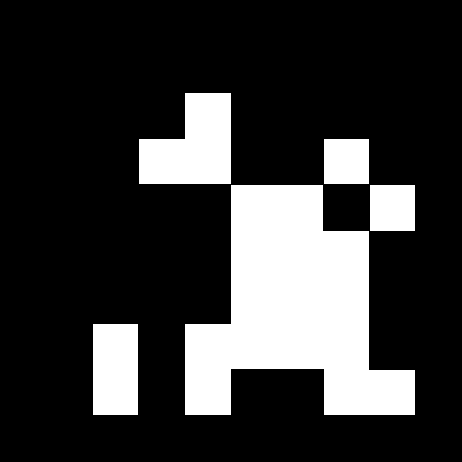
\includegraphics[width=0.8\linewidth]{markers/vector/apriltag_id0.pdf}
        \caption{AprilTag 36h11 (Вектор)}
    \end{minipage}
\end{figure}

\begin{figure}[H]
    \centering
    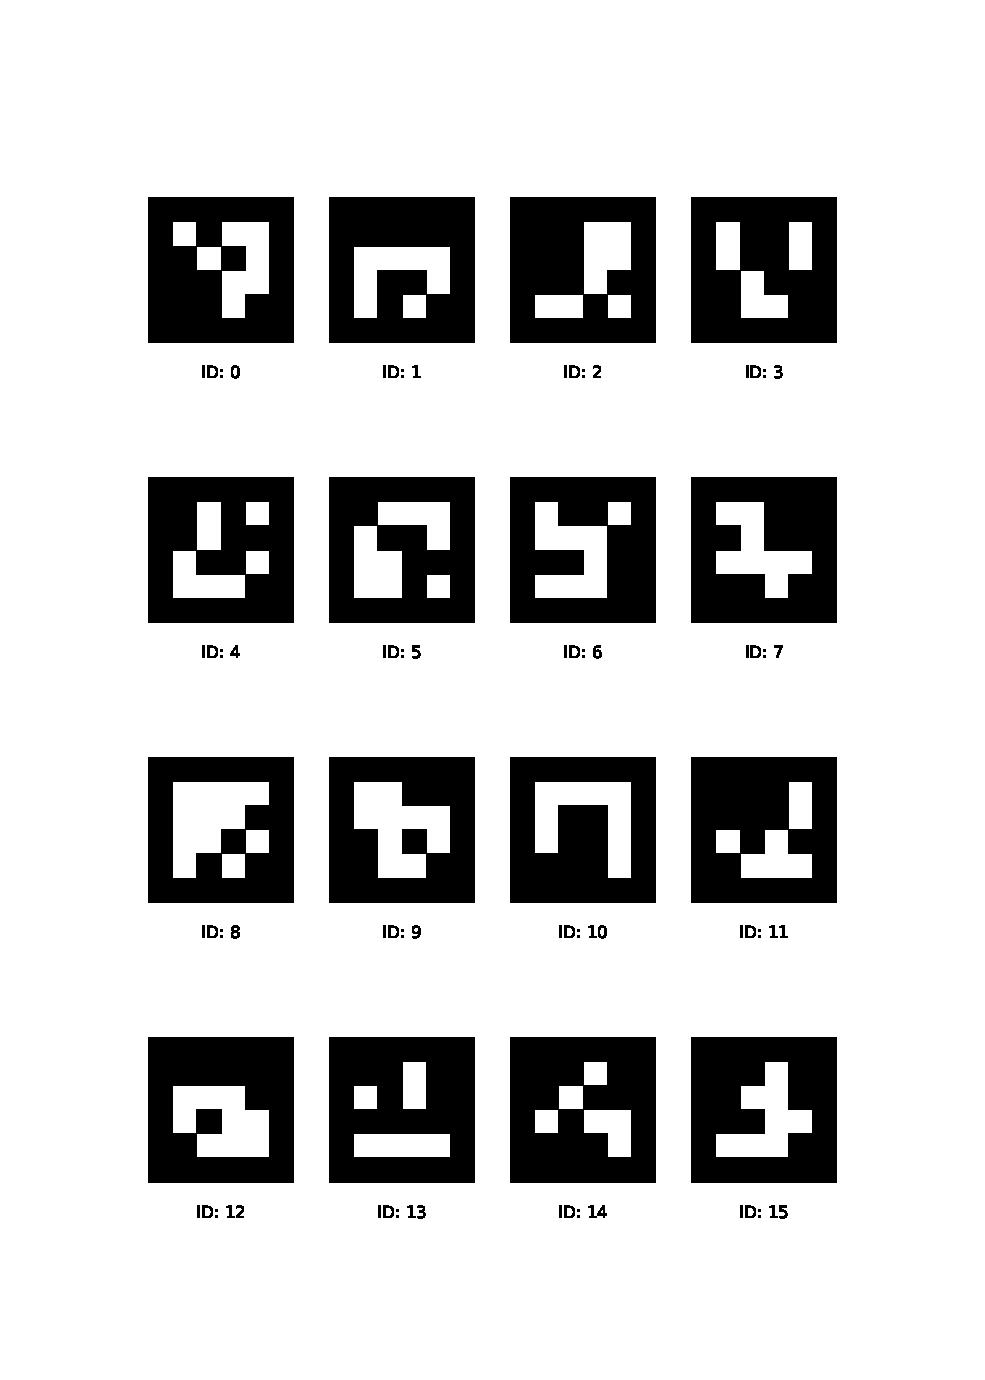
\includegraphics[width=0.9\linewidth]{markers/vector/aruco_grid_4x4.pdf}
    \caption{Карта маркеров 4x4 (ArUco, вектор)}
\end{figure}

\begin{warnbox}{Важно!}
При печати в настройках принтера выберите «Реальный размер» (Actual Size) или «Масштаб 100\%». Иначе размер маркера изменится, и навигация будет врать.
\end{warnbox}

\subsubsection{Требования к монтажу}
\begin{enumerate}
    \item \textbf{Жесткость:} Маркер должен быть идеально плоским. Изгиб бумаги даже на 5 мм приведет к ошибке определения угла (Yaw/Pitch/Roll) на 10-15 градусов. Наклейте маркер на картон, пластик или фанеру.
    \item \textbf{Quiet Zone:} Вокруг черной рамки маркера обязательно должно быть белое поле шириной не менее одного бита. Если наклеить черный маркер на черный пол, он не распознается.
    \item \textbf{Матовое покрытие:} Глянцевая бумага или скотч создают блики от ламп. В месте блика камера видит белое пятно вместо черного пикселя. Используйте матовую ламинацию или матовый скотч.
    \item \textbf{Освещение:} Избегайте размещения маркеров в глубокой тени или напротив ярких окон (контражур).
\end{enumerate}

\subsection{Форматы карт (JSON, XML, KML)}
Карта маркеров — это файл, описывающий положение каждого маркера. Наш инструмент \texttt{19\_map\_creation\_example3\_builder.py} поддерживает несколько форматов.

\begin{codefiletitle}[python]{Инструмент создания карт}{python/advanced_navigation/19_map_creation_example3_builder.py}
\end{codefiletitle}

\subsubsection{JSON (JavaScript Object Notation)}
Основной формат для роботов. Легко читается программами на Python/C++.
\begin{codefiletitle}[python]{Пример карты JSON}{python/advanced_navigation/map_json_example.json}
\end{codefiletitle}

\subsubsection{XML (eXtensible Markup Language)}
Более строгий формат, часто используется в промышленных системах.
\begin{codefiletitle}[xml]{Пример карты XML}{python/advanced_navigation/map_xml_example.xml}
\end{codefiletitle}

\subsubsection{KML (Keyhole Markup Language)}
Формат для отображения на географических картах (Google Earth, QGIS). Позволяет визуализировать схему расположения маркеров поверх спутниковых снимков. Это полезно для планирования полетов на улице.

\subsection{Визуализация и планирование}
Для больших полигонов рекомендуется сначала создать план в CAD-системе или нарисовать схему на миллиметровке, определить координаты установки маркеров, и только потом заносить их в файл карты.

\begin{taskbox}[Задание 3: Калибровка]
Проведите процедуру калибровки камеры Pioneer.
1. Сделайте 20 снимков шахматной доски.
2. Запустите скрипт калибровки.
3. Сравните изображение до и после устранения дисторсии (функция \texttt{cv2.undistort}). Прямые ли линии косяков дверей на краях кадра?
\end{taskbox}

\begin{taskbox}[Задание 4: Создание полигона]
Создайте карту для полета <<восьмеркой>>.
1. Нарисуйте траекторию на полу мелом.
2. Разместите 2 маркера в центрах петель восьмерки.
3. Измерьте их координаты рулеткой относительно точки старта.
4. Создайте JSON файл карты.
\end{taskbox}

\begin{questionbox}[Контрольные вопросы]
\begin{enumerate}
    \item Что такое дисторсия и почему она мешает навигации?
    \item Почему нельзя ламинировать маркеры глянцевой пленкой?
    \item Зачем нужно белое поле вокруг маркера?
    \item В чем преимущество формата KML перед JSON?
\end{enumerate}
\end{questionbox}

\clearpage
\section{Алгоритмы комплексной навигации}

\subsection{Проблема шума и фильтрация}
Данные, получаемые от системы компьютерного зрения, всегда содержат шум. Координаты дрона <<дрожат>> даже если он висит неподвижно. Это происходит из-за дискретности матрицы камеры, изменений освещения и вибраций корпуса.

Если передавать эти <<сырые>> координаты напрямую в полетный контроллер, дрон будет дергаться, пытаясь отработать каждое ложное смещение.

\subsubsection{Фильтр Калмана (Kalman Filter)}
Это стандарт де-факто в робототехнике. Фильтр Калмана не просто усредняет значения, он предсказывает, где дрон \textit{должен} оказаться в следующий момент времени, и корректирует это предсказание на основе новых измерений.

Алгоритм работает циклически в два этапа:
\begin{enumerate}
    \item \textbf{Prediction (Предсказание):} На основе физической модели (скорость, ускорение) мы оцениваем новую позицию. При этом растет неопределенность (мы не уверены в прогнозе).
    \item \textbf{Update (Коррекция):} Мы получаем измерение от камеры. Сравниваем его с прогнозом. Чем точнее датчик (меньше шум измерения $R$), тем больше мы верим ему. Чем точнее наша модель (меньше шум процесса $Q$), тем больше верим прогнозу.
\end{enumerate}

\begin{codefiletitle}[python]{Пример 1D фильтра Калмана}{python/advanced_navigation/kalman_1d_example.py}
\end{codefiletitle}

Выше приведен только ключевой метод \texttt{update()}. Полный запускаемый скрипт с классом \texttt{KalmanFilter1D} и модельным экспериментом находится в файле \texttt{advanced\_navigation/kalman\_filter.py} --- именно его нужно запускать в заданиях ниже.

\subsection{Системы координат}
Одна из самых частых ошибок новичков — путаница в системах координат.

\begin{itemize}
    \item \textbf{Body Frame (Связанная система):} Ось X всегда смотрит вперед (нос дрона), Y — влево/вправо, Z — вверх. Если дрон поворачивается, оси поворачиваются вместе с ним.
    \item \textbf{World Frame / NED (North-East-Down):} Ось X смотрит на Север, Y — на Восток, Z — Вниз (к земле). Эта система неподвижна. Локальная система Пионера, в которой мы задавали точки (раздел~\ref{sec:missions}), тоже неподвижна, но устроена иначе: X вперёд от старта, Y влево, Z \emph{вверх}. Если дрон на старте смотрит на север, при переходе между ними меняются знаки Y и Z.
    \item \textbf{Marker Frame:} Ось Z обычно смотрит перпендикулярно плоскости маркера (вверх от него).
\end{itemize}

Для навигации нам нужно переводить координаты маркера (полученные камерой в Body Frame) в глобальные координаты дрона (World Frame).
$$ Pos_{world} = Pos_{drone} + R_{drone} \cdot Pos_{marker\_relative} $$

\subsection{Точная посадка с PID-регулятором}
Для автоматической посадки на зарядную станцию используется PID-регулятор.
\begin{itemize}
    \item \textbf{P (Proportional):} Чем дальше мы от центра, тем сильнее наклоняемся к нему.
    \item \textbf{I (Integral):} Если нас сносит ветром, мы накапливаем ошибку и наклоняемся сильнее, чтобы компенсировать снос.
    \item \textbf{D (Derivative):} Если мы летим к центру слишком быстро, мы <<тормозим>> заранее, чтобы не пролететь мимо.
\end{itemize}

\begin{taskbox}[Задание 5: Сравнение фильтров]
Запустите скрипт \texttt{kalman\_filter.py}.
1. Измените \texttt{measurement\_noise} (шум измерения) с 0.1 до 5.0. Как ведет себя фильтр?
2. Сравните работу фильтра Калмана и простого скользящего среднего (Moving Average) при резком скачке координат (например, дрон толкнули). Кто быстрее реагирует?
\end{taskbox}

\begin{taskbox}[Задание 6: Посадка в круг]
Напишите скрипт, который:
1. Ищет маркер с высоты 1.5 метра.
2. Снижается до 0.5 метра, удерживая маркер в центре кадра (используя P-регулятор по скоростям $V_x, V_y$ --- команда \verb|set_manual_speed|, раздел~\ref{sec:python-manual-speed}).
3. Если ошибка позиционирования $< 5$ см в течение 2 секунд — совершает посадку.
\end{taskbox}

\begin{questionbox}[Контрольные вопросы]
\begin{enumerate}
    \item Зачем нужен фильтр Калмана, если можно просто взять среднее арифметическое за 10 кадров?
    \item Что произойдет с PID-регулятором, если перепутать знак у коэффициента P?
    \item В какой системе координат (Body или World) камера выдает вектор \texttt{tvec}?
\end{enumerate}
\end{questionbox}

\clearpage
\section{Техническая реализация программных модулей}

В этой главе мы разберем исходный код инструментов, которые используются для создания карт и навигации.

\subsection{Генератор карт (Marker Map Builder)}
Скрипт \texttt{19\_map\_creation\_example3\_builder.py} (глава «Создание навигационных карт») позволяет создавать цифровые карты полигонов и экспортировать их в форматы JSON, XML и KML.

\subsubsection{Структура класса Marker}
Каждый маркер описывается классом \texttt{Marker}, который хранит:
\begin{itemize}
    \item \texttt{id}: Уникальный номер маркера.
    \item \texttt{size}: Физический размер стороны в метрах.
    \item \texttt{x, y, z}: Локальные координаты относительно начала координат карты.
    \item \texttt{yaw}: Угол поворота (ориентация).
    \item \texttt{dictionary}: Тип словаря (например, DICT\_6X6\_250).
\end{itemize}

\begin{codefiletitle}[python]{Класс Marker}{python/advanced_navigation/marker_class_code.py}
\end{codefiletitle}

\subsubsection{Экспорт в XML}
Метод \texttt{save\_xml} генерирует структуру, понятную большинству промышленных систем. Мы используем f-строки для формирования XML-тегов.

\begin{codefiletitle}[python]{Экспорт в XML}{python/advanced_navigation/save_xml_code.py}
\end{codefiletitle}

\subsubsection{Экспорт в KML для Google Earth}
Для отображения маркеров на глобусе Google Earth используется формат KML. Главная сложность здесь — перевод локальных метров $(x, y)$ в глобальные градусы широты и долготы.

Мы используем приближенную формулу (для малых расстояний):
\begin{itemize}
    \item 1 градус широты $\approx 111132$ метра.
    \item 1 градус долготы $\approx 111132 \cdot \cos(\text{широта})$ метров.
\end{itemize}

\begin{warnbox}{Точность GPS}
Данная формула имеет погрешность. Для профессиональной геодезии следует использовать библиотеку \texttt{pyproj} и проекцию UTM.
\end{warnbox}

\subsection{Модуль визуализации}
Для проверки правильности карты полезно отрисовать её на 2D-плоскости перед полетом. Библиотека \texttt{matplotlib} позволяет построить схему расположения маркеров.

\begin{codefiletitle}[python]{Визуализация карты}{python/advanced_navigation/plot_map_code.py}
\end{codefiletitle}

\begin{taskbox}[Задание 7: Свой парсер]
Напишите функцию \texttt{load\_json(filename)}, которая считывает файл карты и создает объекты класса \texttt{Marker}. Проверьте, что карта корректно загружается после сохранения.
\end{taskbox}

\clearpage
\section{Банк практических заданий}

В этом разделе собраны задачи для закрепления материала. Задания разделены по темам и уровням сложности:
\begin{itemize}
    \item \textbf{Базовый (Б):} Проверка понимания основных команд.
    \item \textbf{Продвинутый (П):} Требует написания алгоритмов.
    \item \textbf{Комплексный (К):} Мини-проект, объединяющий несколько тем.
\end{itemize}

\subsection{Блок 1: Работа с камерой и ArUco (aruco\_examples, camera\_examples)}

\begin{enumerate}
    \item \textbf{(Б) <<Фотограф>>:} Напишите скрипт, который делает фото каждые 5 секунд и сохраняет их в папку с текущей датой и временем в названии.
    \item \textbf{(Б) <<Детектор движения>>:} Сравнивайте два последовательных кадра. Если количество изменившихся пикселей превышает порог — выводите сообщение <<Движение обнаружено!>>.
    \item \textbf{(П) <<Умный светофор>>:} Распечатайте красный и зеленый круги. Если дрон видит зеленый цвет — он взлетает на 1 метр. Если красный — садится.
    \item \textbf{(П) <<Поиск маркера>>:} Дрон взлетает и вращается вокруг своей оси (yaw). Как только он видит любой ArUco маркер — останавливается и <<смотрит>> на него 3 секунды.
    \item \textbf{(П) <<Дистанция>>:} Дрон висит напротив маркера. Если маркер приближается (человек подходит с маркером в руках) — дрон отлетает назад, сохраняя дистанцию 1 метр.
    \item \textbf{(К) <<Инвентаризация>>:} В комнате разложены 5 маркеров с ID от 0 до 4. Дрон должен облететь комнату, найти все маркеры и записать в файл: <<ID 3 найден в 12:00>>, <<ID 1 найден в 12:05>>.
    \item \textbf{(К) <<Посадка на платформу>>:} Дрон должен найти маркер на полу, снизиться, зависнуть точно над центром и совершить посадку.
\end{enumerate}

\subsection{Блок 2: Телеметрия (get\_telemetry)}

\begin{enumerate}
    \item \textbf{(Б) <<Черный ящик>>:} Записывайте высоту, заряд батареи и углы наклона (roll, pitch) в CSV файл 10 раз в секунду во время полета.
    \item \textbf{(Б) <<Сигнализация>>:} Если напряжение батареи падает ниже 3.5~В на банку (как в задаче «Умная батарея»), дрон должен включить красную подсветку и начать посадку.
    \item \textbf{(П) <<Альтиметр>>:} Взлетите и висите. Выводите разницу между высотой по барометру и высотой по дальномеру (ToF). В каких ситуациях они отличаются?
    \item \textbf{(П) <<Компас>>:} Напишите программу, которая разворачивает дрон носом строго на Север (0 градусов), затем на Восток (90), Юг (180) и Запад (270).
    \item \textbf{(К) <<Виртуальная стена>>:} Задайте границы зоны полета (например, $X$ от -2 до 2 метров). Если телеметрия показывает выход за границы — дрон должен остановиться и вернуться в центр.
\end{enumerate}

\subsection{Блок 3: Миссии и полет по точкам (mission\_examples)}

\begin{enumerate}
    \item \textbf{(Б) <<Квадрат>>:} Пролетите по точкам $(0,0) \to (1,0) \to (1,1) \to (0,1) \to (0,0)$ на высоте 1 метр.
    \item \textbf{(Б) <<Лестница>>:} Пролетите вперед на 1 метр, набрав 0.5 метра высоты. Повторите 3 раза (как по ступенькам).
    \item \textbf{(П) <<Спираль>>:} Напишите генератор точек для полета по спирали (расширяющийся круг с набором высоты).
    \item \textbf{(П) <<Патруль>>:} Дрон летает между двумя точками бесконечно, пока не увидит препятствие (по датчику расстояния или камере).
    \item \textbf{(К) <<Сканирование поля>>:} Реализуйте полет <<змейкой>> над зоной $3 \times 3$ метра для создания фотоплана местности.
\end{enumerate}

\subsection{Блок 4: Групповой полет (group\_flight\_examples)}

\begin{enumerate}
    \item \textbf{(Б) <<Синхронный старт>>:} Два дрона взлетают одновременно по команде с ПК, висят 5 секунд и садятся.
    \item \textbf{(П) <<Карусель>>:} Два дрона висят напротив друг друга и меняются местами, пролетая по дуге (чтобы не столкнуться).
    \item \textbf{(П) <<Ведущий-ведомый>>:} Первый дрон летит по программе (квадрат). Второй дрон получает телеметрию первого и повторяет его движения со смещением (на 1 метр сзади).
    \item \textbf{(К) <<Шоу дронов>>:} Составьте хореографию для 4 дронов под музыку (используйте мигание светодиодами в такт).
\end{enumerate}

\subsection{Блок 5: Трекинг объектов (PioneerHumanTracking)}

\begin{enumerate}
    \item \textbf{(Б) <<Приветствие>>:} Если дрон видит лицо человека — он мигает зеленым и делает <<кивок>> (pitch вперед-назад).
    \item \textbf{(П) <<Следи за цветом>>:} Возьмите яркий оранжевый мяч. Дрон должен поворачиваться (yaw) так, чтобы мяч всегда был в центре кадра.
    \item \textbf{(П) <<Держи дистанцию>>:} Дрон видит лицо. Если лицо занимает слишком много места в кадре (человек близко) — отлетаем. Слишком мало (человек далеко) — подлетаем.
    \item \textbf{(К) <<Оператор>>:} Дрон летит боком параллельно идущему человеку, снимая его профиль (требует сложной координации движений).
\end{enumerate}

\subsection{Критерии оценки выполнения}
Задание считается выполненным, если:
\begin{enumerate}
    \item Код запускается без синтаксических ошибок.
    \item Дрон выполняет поставленную задачу в реальных условиях не менее 3 раз подряд.
    \item Код содержит комментарии, объясняющие логику работы.
    \item Соблюдены меры безопасности (дрон не вылетает за пределы зоны, экстренная посадка работает).
\end{enumerate}

\clearpage
\section{Типичные ошибки и их устранение}

В процессе работы с дроном часто возникают ситуации, когда <<код правильный, но ничего не работает>>. В этой главе собраны самые частые проблемы.

\subsection{Проблемы с камерой и маркерами}

\subsubsection{Дрон не видит маркер}
\begin{itemize}
    \item \textbf{Причина 1: Плохое освещение.} Камере темно, выдержка увеличивается, появляется <<смаз>> (Motion Blur) при движении.
    \item \textbf{Решение:} Включите дополнительный свет. Маркер должен быть освещен равномерно.
    
    \item \textbf{Причина 2: Блики.} Маркер заламинирован глянцевой пленкой или лежит под лампой.
    \item \textbf{Решение:} Переместите маркер или используйте матовый скотч.
    
    \item \textbf{Причина 3: Неверный размер.} В коде указан размер 0.2 метра, а напечатан маркер 18 см.
    \item \textbf{Решение:} Измерьте черную рамку линейкой и исправьте константу в коде.
    
    \item \textbf{Причина 4: Quiet Zone.} Маркер вырезан по черному контуру без белого поля.
    \item \textbf{Решение:} Наклейте его на белый лист бумаги.
\end{itemize}

\subsubsection{Дрон летит не туда}
\begin{itemize}
    \item \textbf{Причина 1: Перепутаны оси.} Вы думаете, что X — это вправо, а это вперед.
    \item \textbf{Решение:} Проверьте ориентацию (Body Frame). Ось X дрона смотрит вперед --- туда же, куда нос и передняя камера; Y --- влево, Z --- вверх. Не путайте с системой самой камеры в OpenCV: там вперед <<из объектива>> смотрит ось Z (вектор \texttt{tvec}).
    
    \item \textbf{Причина 2: Ошибка калибровки.} Камера <<рыбий глаз>> сильно искажает картинку по краям.
    \item \textbf{Решение:} Проведите калибровку камеры заново.
    
    \item \textbf{Причина 3: Yaw (Рысканье).} Дрон повернулся на 90 градусов, но код продолжает отправлять команды в старой системе координат.
    \item \textbf{Решение:} Используйте глобальную систему координат (World Frame) или учитывайте текущий угол Yaw.
\end{itemize}

\subsection{Проблемы с подключением и Wi-Fi}

\subsubsection{Connection Refused / Timeout}
\begin{itemize}
    \item \textbf{Причина 1:} Компьютер подключился к другой Wi-Fi сети (с интернетом).
    \item \textbf{Решение:} Проверьте, что вы подключены к точке доступа Pioneer\_XXXX.
    
    \item \textbf{Причина 2:} Брандмауэр Windows блокирует порт 8000/8888.
    \item \textbf{Решение:} Разрешите Python доступ в частные сети.
\end{itemize}

\subsection{Ошибки в коде Python}

\subsubsection{IndentationError}
Python очень чувствителен к отступам. Не смешивайте табы и пробелы. Используйте 4 пробела для отступа.

\subsubsection{OpenCV Error: Assertion failed}
Обычно означает, что функция получила пустое изображение (None).
\begin{itemize}
    \item Проверьте, что \texttt{camera.get\_cv\_frame()} не вернул None.
    \item Проверьте, что файл изображения существует (если читаете с диска).
\end{itemize}

\subsection{Аварийные ситуации}

\subsubsection{Дрон не реагирует на Land}
Если программная посадка не срабатывает:
\begin{enumerate}
    \item Не паникуйте.
    \item Нажмите кнопку Disarm в Ground Station (если есть).
    \item Аккуратно поймайте дрон снизу за аккумулятор (берегите пальцы от пропеллеров!) и переверните его вверх ногами. Моторы отключатся автоматически.
\end{enumerate}

\begin{warnbox}{Внимание!}
Никогда не пытайтесь схватить дрон сверху или сбоку — пропеллеры вращаются со скоростью 10 000 об/мин и могут нанести серьезные травмы.
\end{warnbox}

\clearpage

% ============================================================
\part{Приложения}
\appendix
% ============================================================

\section{Справочник Lua API Пионера}
\label{sec:lua-api}

Краткий справочник функций, которыми пользуется книга. Полное описание с примерами --- в справочнике API симулятора (значок книги в заголовке редактора) и в документации Геоскан.

\subsection{Команды автопилота: \texttt{ap}}
\begin{center}\small
\begin{tabularx}{\linewidth}{@{}>{\ttfamily}l X@{}}
\toprule
ap.push(Ev.MCE\_PREFLIGHT) & предстартовая подготовка и запуск моторов; ответ --- \texttt{Ev.ENGINES\_STARTED} \\
ap.push(Ev.MCE\_TAKEOFF) & взлёт на высоту \texttt{Flight\_com\_takeoffAlt}; ответ --- \texttt{Ev.TAKEOFF\_COMPLETE} \\
ap.push(Ev.MCE\_LANDING) & посадка; ответ --- \texttt{Ev.COPTER\_LANDED} \\
ap.push(Ev.ENGINES\_ARM) & запуск моторов без взлёта (проверка) \\
ap.push(Ev.ENGINES\_DISARM) & немедленное выключение моторов \\
ap.goToLocalPoint(x, y, z [, t]) & полёт в точку (метры), необязательно --- за \texttt{t} секунд; ответ --- \texttt{Ev.POINT\_REACHED} \\
ap.updateYaw(rad) & курс в радианах; \texttt{math.rad(deg)} для перевода \\
\bottomrule
\end{tabularx}
\end{center}

\subsection{События: \texttt{Ev} в \texttt{callback(event)}}
\begin{center}\small
\begin{tabularx}{\linewidth}{@{}>{\ttfamily}l X@{}}
\toprule
Ev.ENGINES\_STARTED & моторы запущены после предстарта \\
Ev.TAKEOFF\_COMPLETE & взлёт завершён \\
Ev.POINT\_REACHED & точка \texttt{goToLocalPoint} достигнута \\
Ev.POINT\_DECELERATION & дрон начал торможение перед точкой \\
Ev.COPTER\_LANDED & дрон сел \\
Ev.LOW\_VOLTAGE1 / LOW\_VOLTAGE2 & батарея разряжена: предупреждение / пора садиться \\
Ev.SHOCK & удар, столкновение \\
Ev.CONTROL\_FAIL & потеря управления \\
Ev.ENGINE\_FAIL & отказ мотора \\
\bottomrule
\end{tabularx}
\end{center}

\subsection{Таймеры: \texttt{Timer}}
\begin{itemize}
  \item \verb|Timer.callLater(delay, fn)| --- однократный вызов через \verb|delay| секунд.
  \item \verb|t = Timer.new(period, fn)| --- периодический таймер; \verb|t:start()|, \verb|t:stop()|.
  \item \verb|time()| --- секунды с запуска программы (для измерений).
  \item \verb|sleep(t)| --- блокирующая пауза; в полётных программах не используется.
\end{itemize}

\subsection{Светодиоды: \texttt{Ledbar}}
\begin{itemize}
  \item \verb|leds = Ledbar.new(29)| --- линейка: 4 светодиода платы (\verb|0..3|) и 25 модуля матрицы (\verb|4..28|).
  \item \verb|leds:set(i, r, g, b)| --- цвет светодиода \verb|i|, компоненты \verb|0..1|.
  \item \verb|Ledbar.fromHSV(h, s, v)| --- перевод оттенка (градусы), насыщенности и яркости (проценты) в \verb|r, g, b|.
\end{itemize}

\subsection{Датчики: \texttt{Sensors}}
\begin{center}\small
\begin{tabularx}{\linewidth}{@{}>{\ttfamily}l X@{}}
\toprule
local x, y, z = Sensors.lpsPosition() & положение в локальной системе, м \\
local vx, vy, vz = Sensors.lpsVelocity() & скорость, м/с \\
local yaw = Sensors.lpsYaw() & курс по системе позиционирования, рад \\
local roll, pitch, yaw = Sensors.orientation() & углы ориентации \\
local ax, ay, az = Sensors.accel() & ускорения, м/с$^2$ \\
local gx, gy, gz = Sensors.gyro() & угловые скорости, рад/с \\
local d = Sensors.range() & дальномер: расстояние до поверхности под дроном, м \\
local h = Sensors.altitude() & высота по барометру, м \\
local v = Sensors.battery() & напряжение батареи, В \\
local c1, ..., c8 = Sensors.rc() & восемь каналов пульта, от $-1$ до $1$; \texttt{table.pack(Sensors.rc())} --- в таблицу \\
\bottomrule
\end{tabularx}
\end{center}

\subsection{Идиомы курса}
\begin{itemize}
\item Распаковка: \verb|local unpack = table.unpack|; \verb|leds:set(i, unpack(color))|; \verb|ap.goToLocalPoint(unpack(points[i]))|.
\item «Тернарный»: \verb|local v = cond and A or B|.
\item Счётчик шагов: \verb|nextPoint()| отправляет \verb|points[curr]| и увеличивает \verb|curr|; вызывается из \verb|TAKEOFF_COMPLETE| и \verb|POINT_REACHED|.
\item Конечный автомат: переменная \verb|state| в начале файла (глобальная или \verb|local|) и проверка \verb|event == Ev.X and state == "Y"|; таймеры этапа проверяют \verb|state| первой строкой.
\end{itemize}

\clearpage
\section{Шпаргалка: Lua и Python}
\label{sec:cheatsheet}

Одно и то же действие на двух языках. Lua ждёт событий в \texttt{callback}, Python опрашивает автопилот в цикле.

\begin{center}
\footnotesize
\renewcommand{\arraystretch}{1.2}
\begin{tabularx}{\linewidth}{@{}>{\raggedright\arraybackslash}p{0.18\linewidth} >{\raggedright\arraybackslash}X >{\raggedright\arraybackslash}X@{}}
\toprule
\textbf{Действие} & \textbf{Lua} & \textbf{Python} \\
\midrule
Моторы          & \texttt{ap.push(Ev.MCE\_PREFLIGHT)} & \texttt{pioneer.arm()} \\
Взлёт           & \texttt{ap.push(Ev.MCE\_TAKEOFF)} & \texttt{pioneer.takeoff()} \\
Точка           & \texttt{ap.goToLocalPoint(x, y, z)} & \texttt{pioneer.go\_to\_local\_point(x=, y=, z=, yaw=)} \\
Ждать точку     & \texttt{if event == Ev.POINT\_REACHED} & \texttt{while not pioneer.point\_reached(): time.sleep(0.1)} \\
Курс            & \texttt{ap.updateYaw(рад)} & \texttt{yaw=} в \texttt{go\_to\_local\_point} \\
Посадка         & \texttt{ap.push(Ev.MCE\_LANDING)} & \texttt{pioneer.land()} \\
Выключить моторы & \texttt{ap.push(Ev.ENGINES\_DISARM)} & \texttt{pioneer.disarm()} \\
Пауза           & \texttt{Timer.callLater(t, f)} & \texttt{time.sleep(t)} \\
Периодически    & \texttt{Timer.new(p, f):start()} & цикл \texttt{while} с \texttt{time.sleep(p)} \\
Светодиоды      & \texttt{leds:set(i, r, g, b)}, 0…1 & \texttt{pioneer.led\_control(led\_id, r, g, b)}, 0…255 \\
Позиция         & \texttt{Sensors.lpsPosition()} & \texttt{pioneer.get\_local\_position\_lps()} \\
Дальномер       & \texttt{Sensors.range()} & \texttt{pioneer.get\_dist\_sensor\_data()} \\
Батарея         & \texttt{Sensors.battery()} & \texttt{pioneer.get\_battery\_status()} \\
Кадр камеры     & \texttt{camera.requestMakeShot()} & \texttt{Camera().get\_cv\_frame()} \\
Вывод           & \texttt{print(...)} & \texttt{print(...)} \\
Завершение      & --- & \texttt{pioneer.close\_connection()} \\
\bottomrule
\end{tabularx}
\end{center}

\begin{infobox}[Три главные мысли]
\begin{itemize}
    \item Дрон --- автопилот: вы отдаёте команду и ждёте события, что она выполнена.
    \item В Lua ждут через \texttt{callback(event)}, в Python --- опросом \texttt{while not ...}.
    \item Координаты --- метры от старта, Z вверх, курс в радианах; их показывает \key{Ctrl}+щелчок в симуляторе.
\end{itemize}
\end{infobox}

\clearpage
\section{Аппаратура управления}
\label{sec:rc-control}

В этой главе мы подробно рассмотрим устройство и настройку аппаратуры радиоуправления FlySky FS-i6S, которая входит в стандартный комплект образовательного квадрокоптера «Геоскан Пионер». Пульт дистанционного управления (аппаратура) — это основной инструмент внешнего пилота, позволяющий контролировать полет, переключать режимы работы и выполнять настройку параметров дрона на расстоянии.

Аппаратура работает в паре с приемником, установленным на борту квадрокоптера, передавая команды по радиоканалу. Для корректной работы системы необходимо правильно настроить пульт и установить связь с приемником.

\subsection{Настройка пульта}

Перед первым использованием или после сброса настроек необходимо сконфигурировать пульт управления. Это обеспечит правильную интерпретацию команд полетным контроллером.

Для настройки пульта выполните следующие действия шаг за шагом:

\begin{enumerate}
    \item Вставьте батарейки (4 шт. типа AA) в батарейный отсек и включите пульт дистанционного управления. Для включения необходимо нажать одновременно две кнопки питания (расположены в центре лицевой панели) и удерживать их до включения экрана.
    \item После загрузки на дисплее появится главный экран с отображением текущего состояния, напряжения батарей и положения стиков.
\end{enumerate}

\begin{hintbox}
    \textbf{Подсказка:} В целях безопасности пульт проверяет положение переключателей при включении. Если на экране отображается предупреждение «Warning!!! Place all switches in their up position», это означает, что один из тумблеров находится в активном состоянии или стик газа не в нуле. Приведите все переключатели в верхнее положение (от себя), а левый стик (газ) опустите в самое нижнее положение.
\end{hintbox}

\begin{figure}[H]
    \centering
    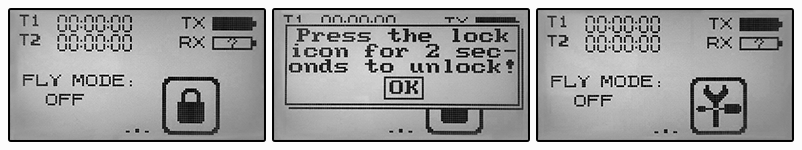
\includegraphics[width=0.8\textwidth]{images/rc_setting_main.png}
    \caption{Главный экран пульта управления FS-i6S}
\end{figure}

\begin{enumerate}
    \setcounter{enumi}{2}
    \item Изначально сенсорный экран заблокирован от случайных нажатий, о чём сигнализирует иконка замка в нижнем правом углу. Для разблокировки нажмите на иконку и удерживайте её в течении 2-4 секунд. После разблокировки иконка сменится на изображение гаечного ключа.
    \item Нажмите на иконку с гаечным ключом, чтобы попасть в меню настроек. Меню разделено на две основные вкладки:
    \begin{itemize}
        \item \textbf{FUNCTION} — здесь производится настройка функций самого пульта (каналы, реверсы и т.д.).
        \item \textbf{SYSTEM} — отвечает за системные настройки связи и приемника.
    \end{itemize}
\end{enumerate}

\subsubsection{Настройки вкладки FUNCTION}

В этой вкладке мы настроим назначение каналов и направление их работы. Это критически важно для того, чтобы движения стиков и переключения тумблеров вызывали ожидаемую реакцию дрона.

Для работы с «Пионером» выполните следующие настройки:

\begin{enumerate}
    \item \textbf{Настройка реверса каналов (Reverse):}
    \begin{itemize}
        \item Перейдите в меню \textbf{REVERSE}.
        \item Установите каналы \textbf{Ch2} (Тангаж) и \textbf{Ch4} (Рыскание) в положение \textbf{Rev} (Реверс). Остальные каналы оставьте в Norm.
    \end{itemize}
    
    \item \textbf{Настройка вспомогательных каналов (Aux. Channels):}
    Для управления режимами полета и дополнительными функциями необходимо назначить физические тумблеры на логические каналы пульта. Перейдите в меню \textbf{AUX. CHANNELS} и настройте каналы следующим образом:
    \begin{itemize}
        \item \textbf{Channel 5:} Нажмите на кнопку выбора канала. В окне \textbf{CH TYPE} выберите \textbf{SWx} (переключатель). Затем нажмите на надпись SwA (по умолчанию) и в открывшемся списке выберите тумблер \textbf{SwC} (трехпозиционный переключатель справа). Этот канал обычно используется для смены режимов полета.
        \item \textbf{Channel 6:} Аналогично настройте на тумблер \textbf{SwD} (крайний правый переключатель).
        \item \textbf{Channel 7:} Настройте на тумблер \textbf{SwB} (трехпозиционный переключатель слева).
        \item \textbf{Channel 8:} Настройте на тумблер \textbf{SwA} (крайний левый переключатель).
    \end{itemize}
\end{enumerate}

\begin{figure}[H]
    \centering
    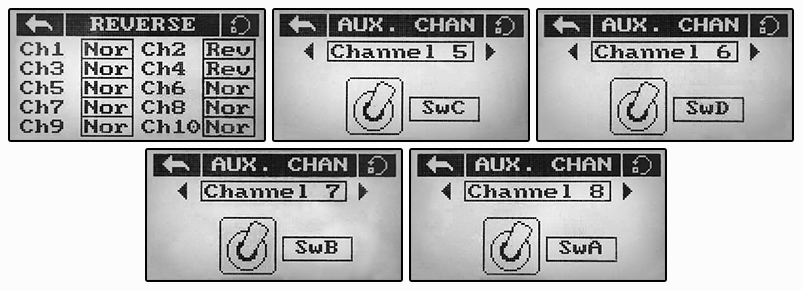
\includegraphics[width=0.8\textwidth]{images/rc_setting_aux.png}
    \caption{Меню настройки вспомогательных каналов}
\end{figure}

\subsubsection{Настройка вкладки SYSTEM}

В этой вкладке задаются параметры протокола передачи данных и режим работы стиков.

\begin{enumerate}
    \item \textbf{Выбор протокола выхода (Output Mode):}
    \begin{itemize}
        \item Перейдите в меню \textbf{OUTPUT MODE}.
        \item Убедитесь, что в поле \textbf{Output} выбран протокол \textbf{PPM}. Полетный контроллер «Пионера» настроен на прием сигналов именно в этом формате. Также должен быть выбран режим \textbf{S.BUS} в поле Serial, если используется соответствующее подключение, но для базовой настройки PPM является основным.
    \end{itemize}
    
    \item \textbf{Режим стиков (Sticks Mode):}
    \begin{itemize}
        \item Перейдите в меню \textbf{STICKS MODE}.
        \item Выберите режим \textbf{M2 (Mode 2)}. В этом режиме левый стик отвечает за Газ (вверх/вниз) и Рыскание (влево/вправо), а правый — за Тангаж (вперед/назад) и Крен (влево/вправо). Это наиболее распространенная схема управления для квадрокоптеров.
    \end{itemize}
\end{enumerate}

\begin{figure}[H]
    \centering
    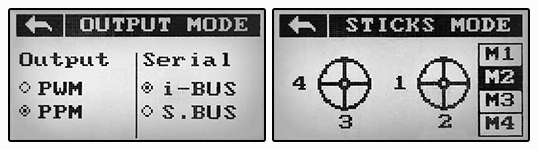
\includegraphics[width=0.8\textwidth]{images/rc_setting_system.png}
    \caption{Системные настройки: выбор режима PPM и Mode 2}
\end{figure}

\subsection{Связь пульта с приемником}

Процедура привязки (Binding) необходима для того, чтобы приемник, установленный на квадрокоптере, «узнал» ваш пульт и реагировал только на его команды. Это исключает пересечение сигналов при полетах нескольких дронов одновременно.

\begin{warnbox}
    \textbf{Внимание:} Для использования квадрокоптера «Пионер Мини» с пультом радиоуправления, в автопилот должны быть загружены соответствующие параметры! Без этого дрон может не реагировать на команды.
\end{warnbox}

\subsubsection{Процедура привязки}

Выполните следующие действия для сопряжения устройств:

\begin{enumerate}
    \item Убедитесь, что приемник (FS-A8S или аналогичный) подключен к плате автопилота.
    \item Найдите на корпусе приемника маленькую кнопку с подписью \textbf{«BIND»}. Нажмите её и \textbf{удерживайте}.
    \item \textbf{Не отпуская} кнопку BIND, подайте питание на квадрокоптер (подключите аккумулятор).
    \item После подачи питания светодиод на приемнике должен начать \textbf{быстро мигать}. Это означает, что приемник перешел в режим привязки. Теперь кнопку можно отпустить.
    \item Включите пульт управления. Зайдите в меню настроек (\textbf{SYSTEM}) и выберите пункт \textbf{RX Bind}.
    \item На экране пульта появится надпись \textbf{Binding to RX...}. В этот момент пульт ищет приемник в режиме привязки.
    \item Как только связь установится, светодиод на приемнике начнет \textbf{мигать медленно}.
    \item Для завершения процедуры нажмите иконку «Назад» ($\leftarrow$) на пульте, чтобы выйти из меню RX Bind.
    \item После выхода из режима привязки светодиод на приемнике должен загореться \textbf{постоянным светом} (красным). Это подтверждает успешное сопряжение и наличие стабильной связи.
\end{enumerate}

\begin{warnbox}
    \textbf{Важно:} Чтобы избежать конфликтов управления, связывайте только один пульт с одним приемником. Если вы меняете пульт или приемник, процедуру привязки необходимо повторить.
\end{warnbox}

\begin{figure}[H]
    \centering
    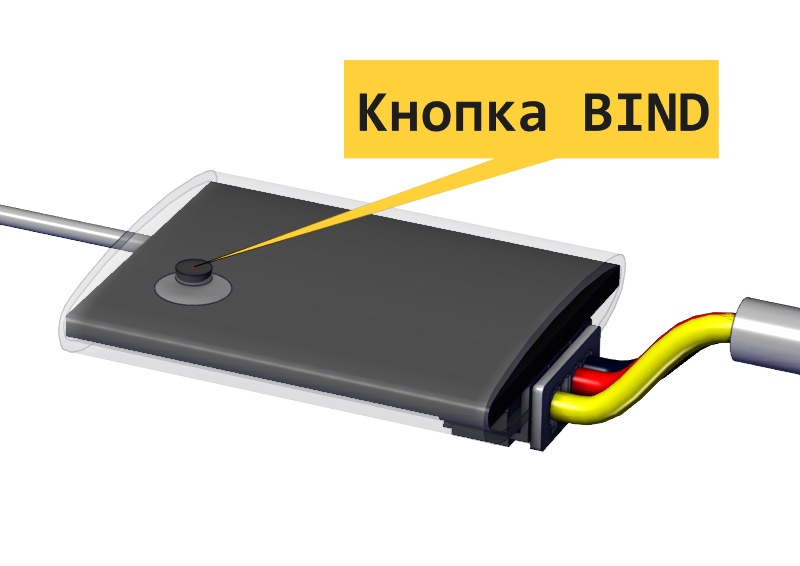
\includegraphics[width=0.6\textwidth]{images/FS-A8S_bind.png}
    \caption{Приемник FS-A8S: расположение кнопки BIND}
\end{figure}

\subsubsection{Возможные проблемы и их решение}

Если после выполнения процедуры квадрокоптер не реагирует на команды:

\begin{itemize}
    \item \textbf{Проверьте протокол:} Зайдите в настройки пульта \textbf{OUTPUT MODE} и убедитесь, что выбран \textbf{PPM}. Другие протоколы (например, PWM или i-BUS) могут не восприниматься текущей прошивкой автопилота без дополнительной настройки.
    \item \textbf{Повторите привязку:} Возможно, вы отпустили кнопку BIND слишком рано или не успели включить режим привязки на пульте. Попробуйте снова.
    \item \textbf{Проверьте параметры:} Если вы летаете на Pioneer Mini, убедитесь через станцию наземного управления, что загружены корректные параметры для работы с RC-пультом.
\end{itemize}

В случае, если выполнить привязку не получается, вы всегда можете обратиться в техподдержку: support@geoscan.aero или в telegram-канал @geoscan\_edu.

\subsection{Стики и тумблеры}

Пульт управления предоставляет пилоту гибкие возможности контроля. Основные органы управления — это два джойстика (стика) и набор переключателей (тумблеров).

\begin{figure}[H]
    \centering
    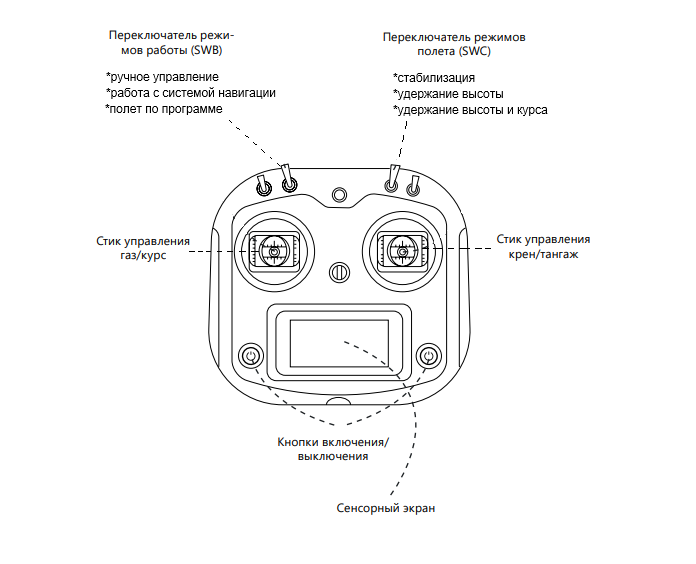
\includegraphics[width=0.8\textwidth]{images/rc_sticks_overview.png}
    \caption{Обзор органов управления пульта FS-i6S}
\end{figure}

\subsubsection{Режимы управления (Тумблеры)}

Тумблеры используются для переключения полетных режимов и активации функций. Ранее мы настроили тумблер \textbf{SwC} (трехпозиционный справа) на 5-й канал.

\textbf{Изменение режима полета (переключатель SwC):}

\begin{itemize}
    \item \textbf{Верхнее положение (Stabilize):} Режим стабилизации. Стик газа напрямую управляет мощностью моторов. Это наиболее «ручной» режим, требующий от пилота постоянного контроля высоты. Подходит для опытных пилотов.
    \item \textbf{Среднее положение (AltHold):} Режим удержания высоты. Квадрокоптер использует барометр для автоматического поддержания заданной высоты. Стик газа в центре — высота не меняется. Стик вверх — набор высоты, вниз — снижение. Это рекомендуемый режим для обучения.
    \item \textbf{Нижнее положение (Headless):} Режим удержания высоты и курса. В дополнение к удержанию высоты, упрощается навигация. Квадрокоптер «запоминает» направление, в котором он был ориентирован при включении моторов (обычно «от пилота»). В полете, независимо от того, куда повернут нос дрона, нажатие стика «вправо» заставит его лететь вправо относительно пилота.
\end{itemize}

\begin{warnbox}
    \textbf{Физика полета:} Для определения высоты полетный контроллер использует барометр, измеряющий атмосферное давление. Помните, что резкие изменения давления (например, открытие окна в помещении или сквозняк) могут быть восприняты дроном как изменение высоты, что приведет к коррекции оборотов моторов.
\end{warnbox}

\textbf{Режимы работы пульта:}
\begin{itemize}
    \item \textbf{Ручное управление:} Вы полностью контролируете дрон с помощью стиков. Режим полета выбирается переключателем SwC.
    \item \textbf{Навигация и GPS:} В режимах с использованием системы навигации или GPS квадрокоптер управляется с пульта, но автоматически удерживает высоту и позицию, если отпустить стики.
    \item \textbf{Полет по программе:} Пионер выполняет загруженную миссию. Вы всегда можете переключить тумблер режимов (например, пощелкать SwC), чтобы перехватить управление и перевести дрон в ручной режим.
\end{itemize}

\subsection{Управление}

Пилотирование квадрокоптера требует координации и понимания того, как каждое движение стика влияет на движение аппарата в пространстве. Рассмотрим управление в режиме \textbf{Mode 2}.

\subsubsection{Управление высотой (Газ / Throttle)}

Левый стик, движение вверх-вниз.

\begin{itemize}
    \item \textbf{Стик вверх:} Обороты моторов увеличиваются, подъемная сила растет, квадрокоптер набирает высоту.
    \item \textbf{Стик вниз:} Обороты уменьшаются, квадрокоптер снижается.
\end{itemize}

\begin{figure}[H]
    \centering
    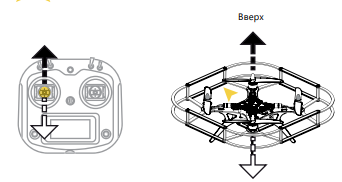
\includegraphics[width=0.45\textwidth]{images/rc_control_1.png}
    
\includegraphics[width=0.45\textwidth]{images/rc_control_2.png}
    \caption{Управление газом: набор высоты и снижение}
\end{figure}

\begin{warnbox}
    \textbf{Важно:} В режиме AltHold (удержание высоты) центр стика соответствует зависанию. Для взлета необходимо поднять стик выше середины.
\end{warnbox}

\subsubsection{Вращение по курсу (Рыскание / Yaw)}

Левый стик, движение влево-вправо.

Отвечает за поворот квадрокоптера вокруг своей вертикальной оси. Это позволяет изменить направление «взгляда» дрона.

\begin{itemize}
    \item \textbf{Стик влево:} Нос квадрокоптера поворачивается влево (против часовой стрелки).
    \item \textbf{Стик вправо:} Нос квадрокоптера поворачивается вправо (по часовой стрелке).
\end{itemize}

\begin{figure}[H]
    \centering
    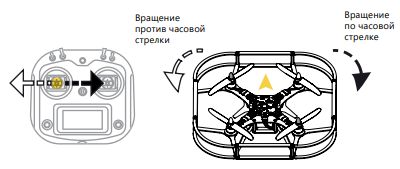
\includegraphics[width=0.75\textwidth]{images/rc_control_3.png}
    \caption{Рыскание: вращение вокруг оси}
\end{figure}

\subsubsection{Тангаж (Pitch) — Движение вперед/назад}

Правый стик, движение вверх-вниз.

Изменяет угол наклона квадрокоптера в продольной плоскости, заставляя его двигаться горизонтально.

\begin{itemize}
    \item \textbf{Стик вверх (от себя):} Нос опускается, дрон летит вперед.
    \item \textbf{Стик вниз (на себя):} Нос поднимается, дрон летит назад.
\end{itemize}

\begin{figure}[H]
    \centering
    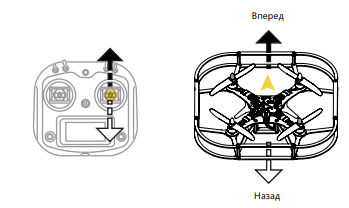
\includegraphics[width=0.75\textwidth]{images/rc_control_4.png}
    \caption{Тангаж: движение вперед и назад}
\end{figure}

\subsubsection{Крен (Roll) — Движение влево/вправо}

Правый стик, движение влево-вправо.

Изменяет угол наклона квадрокоптера в поперечной плоскости, заставляя его смещаться вбок.

\begin{itemize}
    \item \textbf{Стик влево:} Дрон наклоняется влево и летит боком влево.
    \item \textbf{Стик вправо:} Дрон наклоняется вправо и летит боком вправо.
\end{itemize}

\begin{figure}[H]
    \centering
    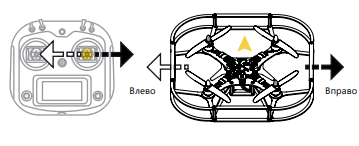
\includegraphics[width=0.75\textwidth]{images/rc_control_5.png}
    \caption{Крен: движение боком}
\end{figure}

\begin{hintbox}
    \textbf{Совет:} При обучении полетам держите хвост квадрокоптера (где установлен аккумулятор или светодиод) к себе. Так направления управления будут совпадать: стик вправо — дрон вправо. Если дрон развернется к вам носом, управление станет «зеркальным» (стик вправо — дрон влево с вашей точки зрения).
\end{hintbox}

\clearpage
\section{Методика тестирования и безопасность}

\subsection{Протокол безопасности полетов}

\subsubsection{1. Подготовка зоны (Pre-flight)}
\begin{itemize}
    \item Очистить зону $3 \times 3$ метра.
    \item Закрыть окна (ветер).
    \item Убрать животных и детей.
    \item Предупредить окружающих о запуске.
    \item Надеть защитные очки (для оператора).
\end{itemize}

\subsubsection{2. Проверка дрона (Checklist)}
\begin{itemize}
    \item \textbf{Пропеллеры:} Целые, затянуты, вращаются свободно.
    \item \textbf{Аккумулятор:} Заряжен > 3.8В на банку, закреплен надежно.
    \item \textbf{Камера:} Линза чистая, шлейф не болтается.
    \item \textbf{Wi-Fi:} Сигнал стабильный (RSS > -60 dBm).
\end{itemize}

\subsubsection{3. Экстренная ситуация}
Если дрон ведет себя неадекватно:
\begin{enumerate}
    \item Громко крикнуть <<ПОСАДКА!>>.
    \item Нажать кнопку LAND (если есть).
    \item Если нет реакции — аккуратно поймать снизу (за батарею) и перевернуть.
    \item Отключить аккумулятор.
\end{enumerate}

\subsection{Тестирование в разных условиях}

\subsubsection{Погодные условия (Ветер)}
Дрон Pioneer очень легкий (около 100 г). Он не предназначен для полетов на улице при ветре > 3 м/с.
Для теста в помещении используйте вентилятор:
\begin{itemize}
    \item Включите вентилятор на минимальную скорость с расстояния 2 метра.
    \item Попробуйте удержать точку (режим Optical Flow).
    \item Если дрон сносит > 50 см — условия непригодны для точной навигации.
\end{itemize}

\subsubsection{Освещение (Lux)}
Камера Pioneer имеет низкий динамический диапазон.
\begin{itemize}
    \item \textbf{Яркое солнце:} Пересвет (белое пятно). Маркеры не видны.
    \item \textbf{Сумерки:} Сильный шум матрицы. Маркеры <<дрожат>>.
    \item \textbf{Мерцание ламп:} Люминесцентные лампы (50 Гц) могут давать полосы на видео.
\end{itemize}

\section{Готовые конфигурации (Templates)}

\subsection{Файл конфигурации camera\_params.yaml}
Те же параметры камеры, что сохраняют скрипты калибровки в \texttt{data.yml}, но в формате для сторонних инструментов: матрица --- \texttt{camera\_matrix}, дисторсия --- \texttt{distortion\_coefficients}. Примеры этой книги читают \texttt{data.yml}.
\begin{codefiletitle}[bash]{camera_params.yaml}{python/advanced_navigation/camera_params_yaml.yaml}
\end{codefiletitle}

\subsection{Шаблон скрипта полета (main.py)}
\begin{codefiletitle}[python]{Базовый шаблон}{python/advanced_navigation/main_template_py.py}
\end{codefiletitle}

\clearpage

\nocite{*}
\printbibliography[heading=bibintoc, title={Список литературы}]

\end{document}
